
%%------------------------------------------------------------
%Ecuaciones ordinarias
%==============================================================
%=============================================================

\documentclass[12pt]{book}

%----------------------------------------------------------------
%PAQUETES
\usepackage{mflogo}
\usepackage{amssymb,amsmath}
\usepackage[dvips]{graphicx}
\usepackage{makeidx}
%\usepackage{psfrag}
%\usepackage{diagrams}
\usepackage{theorem}
\usepackage[spanish, activeacute]{babel}
%\usepackage{fancybox}
\usepackage{times}
\usepackage{fancyhdr}
\usepackage{pstricks-add}
\usepackage[cp1252]{inputenc}

%%%%%%%%%Estilo de la pagina%%%%%%%%%%%%%%%%%%%%%%%%%%%%%%%%%%%
%%%%%%%%%%%%%%%%%%%%%%%%%%%%%%%%%%%%%%%%%%%%%%%%%%%%%%%%%%%%%%%%%%

\pagestyle{fancyplain}


\renewcommand{\sectionmark}[1]
                {\markright{\thesection\ #1}}


\lhead[\fancyplain{}{\bfseries\thepage}]
      {\fancyplain{}{\bfseries\rightmark}}

\rhead[\fancyplain{}{\bfseries\leftmark}]
      {\fancyplain{}{\bfseries\thepage}}

\cfoot{}


%--------------------------------------------------------------
%DEFINICIONES del Estilo de los TEOREMAS

 %\theoremstyle{marginbreak} \theoremheaderfont{\scshape}


\newtheorem{teorema}{Teorema}[section]
\newtheorem{lema}[teorema]{Lema}
\newtheorem{corolario}[teorema]{Corolario}
\newtheorem{proposicion}[teorema]{Proposici\'on}
\newtheorem{definicion}[teorema]{Definici\'on}


%\theoremstyle{plain}

        {\theorembodyfont{\rmfamily}
\newtheorem{ejemplo}[teorema]{Ejemplo}
\newtheorem{ejercicio}{Ejercicio}[chapter]
}


%-------------------------------------------------------------
%-------------------------------------------------------------
%DOCUMENTO
%============================================================

%\includeonly{uni5}


%-------------------------------------------------------------
\makeindex
%-------------------------------------------------------------
%DOCUMENTO
%============================================================



\begin{document}

%=========================================
%PARAMETROS
%==========================================
%\sboxsep5pt

%=======================================================================
%DEFINICIONES COMANDOS
%======================================================================
\newcommand{\nn}{\mathbb{N}}
\newcommand{\rr}{\mathbb{R}}
\newcommand{\C}{\overline}
\renewcommand{\chaptername}{Unidad}
\newcommand{\resa}[1]{\emph{#1}\index{#1}}
\newcommand{\p}{\varphi}
\newcommand{\oo}{\Omega}
%\newcommand{\sen}{\hbox{sen }}
%=============================================================================
%NUEVOS ENTORNOS
%============================================================================

\newenvironment{demo}{\noindent\emph{Dem.}}{$\square$ \newline\vspace{5pt}}
%--------------------------------------------------------------
\begin{center}
\begin{Huge}
   Ecuaciones Diferenciales Ordinarias
\end{Huge}

\begin{Large}

\vspace{1cm}

Fernando Mazzone
\end{Large}

\vspace{1in}



\end{center}




\tableofcontents





%=====================================================================
%CAPITULO I
%=======================================================================
\chapter{Cardinalidad} En esta unidad estudiaremos el concepto de
cardinalidad de un conjunto. Con este concepto se pretende darle
un entendimiento a la noci\'on de cantidad de elementos de un
conjunto, en especial cuando este es ``infinito''. Como se ver\'a,
y por extra\~no que parezca, aunque el conjunto involucrado sea
``infinito'', de todas maneras podremos definir el cardinal de ese
conjunto, con esto implicitamente decimos que no todos los
conjuntos infinitos tendr\'an el mismo cardinal. Empezaremos
recordando algunas cuestiones b\'asicas de teor\'{\i}a de
conjuntos que, a la vez, nos servir\'an como referencia para  las
notaciones.

%--------------------------------------------------------------
%SECCION




\section{Repaso de lo b\'asico sobre conjuntos}
La siguiente introducci\'on est\'a lejos de ser exhaustiva, solo
recordaremos conceptos ya sabidos. Nos dentendremos algo m\'as en
aquellos puntos que puedan ser nuevos.

\begin{definicion}Dados dos conjuntos $A$ y $B$ denotaremos su uni\'on,
intersecci\'on y diferencia por: $A\cup B$, $A\cap B$ y $A-B$
repectivamente. Estos nuevos conjuntos se definen por:
\[A\cup B=\{x:x\in A\vee x\in B\},\]

\[A\cap B=\{x:x\in A\wedge x\in B\}\]
y

\[A-B=\{x:x\in A \wedge x\notin B\},\]
respectivamente.
\end{definicion}
 Por lo general, tendremos que los
conjuntos con los que trabajaremos estar\'an contenidos en un
conjunto que llamaremos el universo $\mathcal{U}$. Aceptado la
existencia de este universo, frecuentemente usaremos la siguiente
notaci\'on para el complemento
\[A^c=\mathcal{U}-A.\]
Adem\'as consideraremos la operaci\'on de diferencia sim\'etrica,
defini\'endose esto por:
\[A\bigtriangleup B=(A-B)\cup(B-A).\]

\begin{definicion}Dados dos elementos arbitrarios $a$ y $b$ se
define el par ordenado $(a,b)$, por la siguiente igualdad
\[(a,b)=\{a,\{a,b\}\}.\]
\end{definicion}

La propiedad m\'as relevante de pares ordenados es que si
$(a,b)=(c,d)$ entonces $a=c$ y $b=d$. Ahora consideramos el
conjunto formado por todos los pares ordenados de elementos
pertenecientes a conjuntos dados.

\begin{definicion} Sean $A$ y $B$ conjuntos. El producto cartesiano de $A$ con
$B$, denotado por $A\times B$, es el siguiente conjunto:
\[A\times B=\{(a,b):a\in A\wedge b\in B\}.\]
\end{definicion}
La siguiente definici\'on es bien conocida.

\begin{definicion} Una funci\'on $f$ de $A$ en $B$ (abreviaremos esta frase
porel siguiente s\'{\i}mbolo: $f:A\longrightarrow B$), es un
subconjunto del producto cartesiano $A\times B$ con la propiedad
que: para todo $a\in A$ existe un \'unico $b\in B$ tal que
$(a,b)\in f$. \end{definicion}

Suponemos que ya todos conocemos estos conceptos, asi como los
conceptos relacionados de: imagen, la notaci\'on $f(a)$, funci\'on
inyectiva, suryectiva y biyectiva. Admitimos todo esto por sabido.
Ahora introducimos una nueva notaci\'on.

\begin{definicion}
Por $B^A$ denotamos al conjunto de todas las funciones
$f:A\longrightarrow B$.
\end{definicion}

Mas adelante daremos algunas explicaciones del porque de esta
notaci\'on.

Seguidamente damos las definiciones, que pueden no haberse usado
antes, de los conjuntos imagen y preimagen, de un conjunto dado,
por una funci\'on, tambi\'en, dada.

\begin{definicion} Dada una funci\'on $f:A\longrightarrow B$ y subconjuntos
$C\subset A$ y $D\subset B$ definimos:
\[f(C)=\{f(a):a\in C\}\]
y
\[f^{-1}(D)=\{a\in A:f(a)\in C\}.\]
\end{definicion}

Las figuras \vref{figura1} y \vref{figura2} aclaran el significado
de estos conjuntos.


\begin{figure}[h]

\begin{center}

\psfrag{A}{$A$}

 \psfrag{B}{$B$}

 \psfrag{C}{$C$}
 \psfrag{f(C)}{$f(C)$}
 \psfrag{f}{$f$}


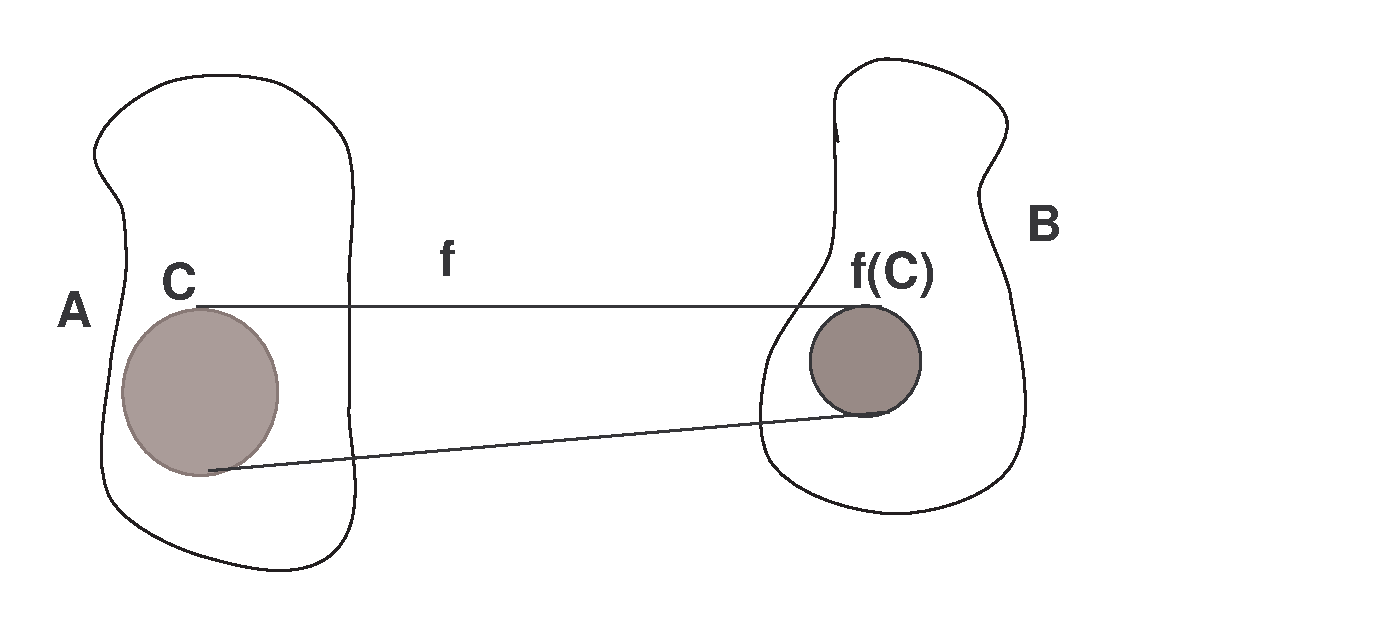
\includegraphics[height=5cm, width=10cm]{funcima.eps}


 \caption{Conjunto $f(C)$}\label{figura1}

\psfrag{A}{$A$}

 \psfrag{B}{$B$}

 \psfrag{D}{$D$}
 \psfrag{f-1(D)}{$f^{-1}(D)$}
 \psfrag{f}{$f$}


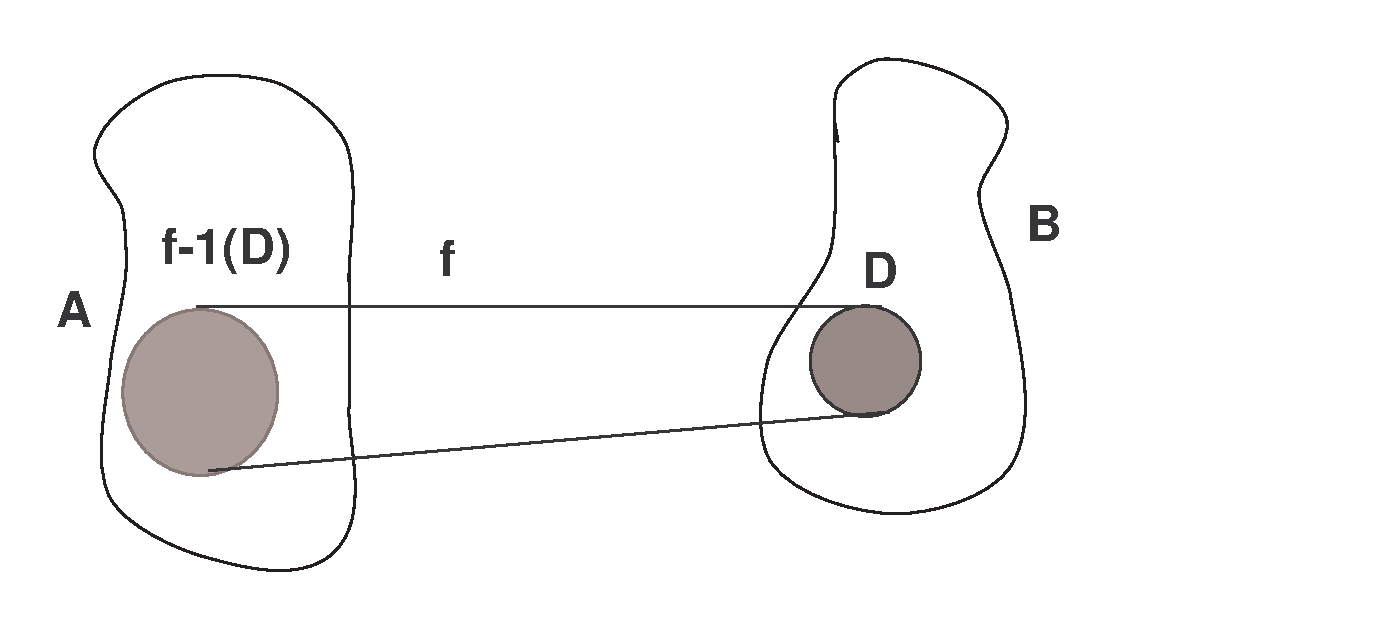
\includegraphics[height=5cm, width=10cm]{fpreima.eps}


 \caption{Conjunto $f^{-1}(D)$}\label{figura2}


\end{center}

\end{figure}





Muy a menudo utilizaremos las propiedades que a continuaci\'on se
enuncian. Las demostraciones, de las mismas, quedaran a cargo del
alumno; ver Ejercicio \vref{3}.

\begin{proposicion}\label{propfunc} Sea $f:A\longrightarrow B$ una funci\'on.
Entonces
\begin{itemize}
\item[1.] $f(C_1\cup C_2)=f(C_1)\cup fe(C_2).$
\item[2.]$f^{-1}(D_1\cup D_2)= f^{-1}(D_1)\cup f^{-1}(D_2).$
\item[3.] $f(C_1\cap C_2)\subset f(C_1)\cap f(C_2).$
\item[4.]$f^{-1}(D_1\cap D_2)= f^{-1}(D_1)\cap f^{-1}(D_2).$
\end{itemize}
\end{proposicion}


Tambi\'en vamos a considerar el conjunto de partes de un conjunto
dado, esto es el conjunto de todos sus subconjuntos.
Expl\'{\i}citamente:
\[\mathcal{P}(A)=\{C:C\subset A\}.\]
Se pueden efectuar uniones e intersecciones de una cantidad
arbitraria de conjuntos. Para poder enunciarlas debemos definir
antes lo que entendemos por una \emph{familia subindicada de
conjuntos} (o brevemente \emph{familia de conjuntos}).

\begin{definicion} Supongamos dado un conjunto $I$, al que nos referiremos como
conjunto de \'{\i}ndices, y una funci\'on $F:I\longrightarrow
\mathcal{P}(A)$. As\'{\i} tenemos que, para cada $i\in I$, existe
un \'unico subconjunto de $A$, que llamaremos\footnote{Observar
que esto es posible puesto que tenemos una dependencia funcional
de los subconjuntos de $A$ con los elementos de $I$} $A_i$ tal que
$f(i)=A_i$. Diremos entonces que $\{A_i\}_{i\in I}$ es una familia
subindicada de conjuntos por el conjunto de \'{\i}ndices $I$.
\end{definicion}

Ahora podemos definir la uni\'on y la intersecci\'on de una
familia de esta \'{\i}ndole de la siguiente manera
\begin{definicion} Definimos la uni\'on e intersecci\'on de una
familia $\{A_i\}_{i\in I}$ por:
\[\bigcup_{i\in I}A_i=\{a:\exists i\in I:a\in A_i\}\]
y
\[\bigcap_{i\in I}A_i=\{a:\forall i\in I:a\in A_i\}\]
respectivamente.
\end{definicion}
En el Ejercicio \vref{propuniarb} podemos encontrar una seria de
propiedades de uniones e intersecciones de familias de conjutos.
Estas propiedades las usaremos con frecuencia.
 Por \'ultimo, en esta revisi\'on de conjuntos, expondremos el
 axioma de elecci\'on. Este es un axioma de la teor\'{\i}a de
 conjuntos. Hay que aclarar que es posible axiomatizar la
 teor\'{\i}a de conjuntos, de esta axiomatizaci\'on el mencionado axioma
 puede formar parte. Decimos ``puede'' por que este
 axioma ha despertado multitud de controversias en torno a su
 inserci\'on o no en el restante conjunto de axiomas. No vamos a
 discutir aqu\'{\i} esta controversia ni tampoco la teor\'{\i}a
 axiom\'atica de conjuntos pues esto nos desviar\'{\i}a de nuetros
 objetivos. Solo enunciaremos el axioma de elecci\'on, que
 usaremos frecuentemente.

\begin{axioma} Sea $\{A_i\}_{i\in I}$ una familia de conjuntos no
vacios. Entonces existe una funci\'on
\[f:I\longrightarrow\bigcup_{i\in I}A_i.\]
con la propiedad  que: $\forall i\in I$
\[f(i)\in A_i.\]
\end{axioma}



%--------------------------------------------------------------
%SECCION


\section{Definici\'on de conjuntos coordinables}
En esta secci\'on definimos el concepto clave de esta unidad, a
saber el concepto de que dos conjuntos sean coordinables. Damos
una breve discuci\'on para motivar nuestra definici\'on.

 Cuando
algui\'en cuenta alg\'un conjunto de cosas, establece una
correspondencia entre los objetos que cuenta y un subconjunto de
n\'umeros naturales... veamos como. En el proceso de conteo,
alg\'un objeto fue el primero en contarse, y se habr\'a dicho:
``uno'' para ese objeto. El proceso continua asignando,
sucesivamente, el n\'umero dos, tres, etc, a los restantes objetos
a contar, hasta que no queden m\'as por contarse. As\'{\i}, si en
este proceso llegamos hasta el 20, por ejemplo, decimos que hay 20
objetos. Aunque no haya que percatarse de eso a los fines
pr\'acticos, lo que tambi\'en hicimos fue: Establecer una
correspondencia o funci\'on entre los objetos y el conjunto
$\{1,\dots,20\}$. M\'as a\'un, esta correspondencia fue biyectiva
pues: A cada n\'umero le correspondi\'o solo uno de los objetos
(es decir: La funci\'on es inyectiva) y a cada objeto le
correspondi\'o alg\'un n\'umero (es decir: La funci\'on es
suryectiva). En otras palabras contar un conjunto significa:
determinar el \emph{intervalo inicial del conjunto} de los
n\'umeros naturales\footnote{Por esto se entiende un conjunto de
la forma: $\{j\in\mathbb{N}:1\leq j\leq n\}$, para cierto
$n\in\mathbb{N}$. De ahora en m\'as, llamaremos a este conjunto:
$\mathbb{N}_n$} para el cual exista una correspondencia biyectiva
con el conjunto que queremos contar. Conocer esto obviamente es
in\'util a los efectos de contar cosas de la ``vida cotidiana'';
no obstante, es una observaci\'on fundamental a los efectos de
extender lo que llamamos ``contar'' a conjuntos infinitos. Lo que
antecede sugiere la siguiente definici\'on.

\begin{definicion}\label{defcoordinables} Dados dos conjuntos: $A$ y $B$,
se dir\'a que ellos son coordinables, escribiremos $A\thicksim B$,
si existe una funci\'on biyectiva $f:A\longrightarrow B$.
\end{definicion}

Esta es nuestra definici\'on de que dos conjuntos, ``finitos'' o
no, tengan ``la misma cantidad de elementos''. Como veremos, no
todos los  conjuntos ``infititos'' son coordinables entre si.

Es bueno notar que no es dif\'{\i}cil demostrar que $\thicksim$ es
una relaci\'on de equivalencia (ver Ejercicio \vref{1}).

 Ahora
veamos algunos ejemplos.

\begin{ejemplo}Consideremos la funci\'on
$f:\nn\longrightarrow\{x\in\nn:x\,\,\text{es par}\}$, definida por
$f(x)=2x$. Facilmente se ve que $f$ es una biyecci\'on entre los
conjuntos indicados. De ah\'{\i} que:
$\nn\thicksim\{x\in\nn:x\,\,\text{es par}\}$.
\end{ejemplo}

En este ejemplo observamos que, desde nuestro punto de vista, el
conjunto de los naturales tiene ``la misma cantidad de elementos''
que el conjunto de los naturales pares. Es decir, en este caso, el
todo no es mayor que una de sus partes.

\begin{ejemplo}\label{rcoord(0,1)} Veamos que $\rr\thicksim (0,1)$. En este caso se
puede considerar la funci\'on

\[f(x):= \tan\biggl(\frac{2\pi x-\pi}{2}\biggr).\]
Dejamos como ejercicio corroborar que la funci\'on dada establece
una biyecci\'on entre los conjuntos involucrados.
\end{ejemplo}

Los dos ejemplos anteriores muestran una caracter\'{\i}stica
importante de los conjuntos ``infinitos''; un subconjunto de ellos
puede ser coordinable con el conjunto total. Mientras que, los
conjuntos ``finitos'' parecen carecer de esta caracter\'{\i}stica.
Ver Ejercicio \vref{infcoordconsub}




%--------------------------------------------------------------
%SECCION

\section{Conjuntos numerables}
Hasta el momento empleamos comillas para encerrar los t\'erminos:
finito e infinito. Esto se debe a que estamos en condiciones, a
partir de la noci\'on  de coordinalidad, de definir de forma
precisa el significado de estos t\'erminos.

\begin{definicion} Diremos que un conjunto $A$ es:
\begin{itemize}
\item[1.] \textbf{finito} si existe un $n\in\nn$ tal que
$A\thicksim\nn_n$.
\item[2.] \textbf{infinito }si no es finito.
\item[3.] \textbf{numerable} si $A\thicksim\nn$.
\item[4.] \textbf{a lo sumo numerable} si es finito o numerable.
\end{itemize}
\end{definicion}

En virtud de que $\thicksim$ es una realci\'on de equivalencia, y
especialmente por el car\'acter transitivo de esta, si $A\thicksim
B$ y $B$ tiene alguna de las cuatro propiedades de la definici\'on
anterior entonces $A$ tendr\'a esa misma propiedad.

Recordemos que, por definici\'on, una sucesi\'on $\{a_i\}$ de
elementos de un conjunto $A$ es una funci\'on
$f:\nn\longrightarrow A$, donde $a_i=f(i)$. Vemos as\'{\i} que el
concepto de numerabilidad est\'a relacionado con el de sucesi\'on.
En efecto, si el conjunto $A$ es numerable entonces sus elementos
se pueden disponer en una sucesi\'on, donde ning\'un t\'ermino se
repita.

Es oportuno que observemos que un conjunto no puede ser numerable
y finito a la vez; dicho de otra forma, los conjuntos numerables
son infinitos. Esto, como hemos definido los conceptos numerable y
finito de  manera precisa, tiene que ser demostrado.

\begin{teorema}\label{nesinfinito} Un conjunto numerable es
infinito.
\end{teorema}
\begin{demo} Supongamos que, por lo contrario, existe un conjunto
$A$ numerable y, a la vez, finito. As\'{\i} tendr\'{\i}amos que:
$A\thicksim\nn$ y $A\thicksim\nn_n$, para alg\'un $n\in\nn$. Como
$\thicksim$ es una relaci\'on de equivalencia , deducimos que
$\nn\thicksim\nn_n$. Sea, pues, $f$ una biyecci\'on:
$f:\nn_n\longrightarrow\nn$. Ahora consideremos el
natural\footnote{El s\'{\i}mbolo $:=$ se lee \emph{igual por
definici\'on}. Esto es, el miembro de la izquierda es definido por
el de la derecha}: $k:=f(1)+\dots+f(n)+1$. Como $f$ es una
biyecci\'on, existe alg\'un $m$, con $1\leq m\leq n$ tal que
$f(m)=k$. Es decir
\[f(m)=f(1)+\dots+f(n)+1.\]
Seguramente, en el miembro derecho, uno de los t\'erminos es
$f(m)$. Este se puede cancelar con el miembro de la izquierda,
quedando
\[0=f(1)+\dots+f(m-1)+f(m+1)+\dots+f(n)+1.\]
Esta igualdad es absurda pues el miembro de la derecha es mayor
que $1$.
\end{demo}

Vamos a ver algunos otros conjuntos que tambi\'en son numerables.
Empezamos por el siguiente.

\begin{proposicion}\label{subconjunto} Un subconjunto de un conjunto a lo sumo numerable es a
lo sumo numerable.
\end{proposicion}
\begin{demo} Sea $A\subset B$, con $B$ a lo sumo numerable. Se puede suponer
que $B\subset \nn$. ?`Por qu\'e? Y, tambi\'en podemos suponer que
$A$ es infinito, puesto que si fuera finito no habr\'{\i}a nada
que probar. Definimos una funci\'on $f:\nn\longrightarrow A$ por
induccion. Puesto que los n\'umeros naturales son bien ordenados,
tenemos que $A$ tiene un primer elemento, digamos, $a_1$.
Definamos
\[f(1)=a_1.\]
Ahora definimos $f(j)$ por:
\begin{equation}\label{frecursiva}
f(j)=\text{el primer elemento del conjunto: }A-\{f(i):1\leq i\leq
j-1\}. \end{equation} Esta definici\'on es posible pues
$A-\{f(i):1\leq i\leq j-1\}\neq\emptyset$, de lo contrario $A$
ser\'{\i}a finito. Queda as\'{\i} definida la funci\'on $f$. Resta
ver que es biyectiva.

Veamos, en primer lugar, que es inyectiva. Sea $i>j$. En virtud de
~\eqref{frecursiva}, tenemos que $f(i)\notin\{f(k):1\leq k\leq
i-1\}$ de lo cual, y como $j<i$, deducimos que $f(i)\neq f(j)$.

Ahora veamos la suryectividad. Supongamos que existe un elemento
$n\in A$ tal que $n\notin f(\nn)$. Recordemos la Definici\'on
\eqref{frecursiva}. Ella nos dice, en virtud de que $n\notin
f(\nn)$, que $f(i)<n$, para todo $i$. Esto es debido a que $f(i)$
es el m\'{\i}nimo del conjunto $ A-\{f(k):1\leq k\leq i-1\}$ y a
que $n$ pertenece a ese conjunto. Tenemos, entonces, que
$f(\nn)\subset\nn_n$. Como consecuencia del Ejercicio \vref{1.5}
conclu\'{\i}mos que $f(\nn)$ es finito. Pero como $f$ es inyectiva
$\nn\thicksim f(\nn)$. Lo que es una contradicci\'on pues $\nn$ es
infinito.
\end{demo}

\begin{proposicion}\label{zesnum}
El conjuntos $\mathbb{Z}$, de los enteros,  es numerable.
\end{proposicion}
\begin{demo} Constru\'{\i}mos una funci\'on que establece
una biyecci\'on entre: Los enteros positivos y los naturales pares
y entre los enteros negativos y los naturales impares. La
funci\'on es la siguiente:

\[f(x)=\left\{
\begin{array}{ll}
    2x+2, & \hbox{si $x\geq 0$;} \\
    -2x-1, & \hbox{si $x<0$.} \\
\end{array}
\right.\] Dejamos como ejercicio demostrar que, efectivamente, la
funci\'on $f$ es una biyecci\'on entre $\nn$ y $\mathbb{Z}$.
\end{demo}

\begin{proposicion}\label{NxNesnum} El conjunto $\nn\times\nn$ es numerable.
\end{proposicion}
\begin{demo} La demostraci\'on de este enunciado ya no es tan
sencilla. La idea se la debemos a G. Cantor. Daremos una idea de
la construcci\'on de la biyecci\'on entre $\nn\times\nn$
 y $\nn$. En rigor de verdad, a los efectos l\'ogicos de la demostraci\'on, todo lo que sigue
 se podr\'{\i}a obviar; pudi\'endose dar la f\'ormula
 ~\eqref{forfinal} sin dar ninguna justificaci\'on de como se nos
 ocurri\'o. Elegimos el camino contrario, explicar
 como obtener la f\'ormula.


 Dispongamos del conjunto $\nn\times\nn$ en un arreglo del tipo
de una ``matr\'{\i}z infinita'', como sigue:
\[\begin{diagram}
(1,1)   & \rTo        & (1,2)  &                      & (1,3)  &                      & (1,4) &\dots\\
        & \ldTo(2,2)  &        &\ldTo(2,2)\ruTo(4,2)  &        & \ldTo(2,2)\ruTo(6,4) &        &     \\
(2,1)   &             & (2,2)  &                      & (2,3)  &                      &        &      \\
        &\ldTo(2,2)   &        & \ldTo(2,2)           &        & \ddots               &        &      \\
(3,1)   &             &(3,2)   &                      &        &                      &        &      \\
        & \ldTo(2,2)  &        &   \ddots             &        &                      &        &      \\
 (4,1)  &             &        &                      &        &                      &        &      \\
 \vdots &             &        &                      &        &                      &        &      \\
\end{diagram}\]
Notar que, adem\'as de colocar los pares ordenados, hemos colocado
algunas flechas. Estas flechas indican un ``camino''; este es el
camino que seguiremos  para enumerar los pares ordenados.
As\'{\i}, construiremos una funci\'on $f$ que har\'a las
siguientes asignaciones:

\begin{eqnarray}
    f:\nn\times\nn&\longrightarrow\nn\nonumber \\
    (1,1)&\longmapsto 1\nonumber \\
    (1,2)&\longmapsto 2\nonumber \\
     (2,1)&\longmapsto 3\nonumber\\
        &\hspace{-29pt}\vdots\nonumber \\
        \nonumber
\end{eqnarray}
Observar que, en nuestro ``camino'', vamos siguiendo diagonales de
la matriz, de izquierda a derecha y de arriba hacia abajo. Cuando,
siguiendo el camino, llegamos al margen izquierdo de la matriz
``saltamos'' al borde superior, para luego ``descender'' por la
siguiente diagonal. Estas diagonales tienen $1, 2, 3, \dots$
elementos. Agrupemos los n\'umeros naturales de esa forma, es
decir un primer grupo de uno, un segundo de dos y as\'{\i}
indefinidamente:

\[\underbrace{1}_{1} \underbrace{2\quad 3}_{2}\quad\underbrace{4\quad 5\quad
6}_{3}\quad \underbrace{7\quad 8\quad  9\quad 10}_{4}\dots
\]
Obs\'ervese que

\begin{equation}\label{numfinal}
\frac{j(j +1)}{2}=\text{n\'umero final del agrupamiento
$j$-\'esimo}.
\end{equation}
Por ejemplo: el grupo cuarto tiene por su \'ultimo elemento el 10,
que es igual a 4.5/2. Tambien tenemos que todos los pares
ordenados sobre la misma diagonal, tienen la caracter\'{\i}stica
de que sus componentes suman lo mismo. Numeremos las diagonales,
de izquierda a derecha, empezando por 1. As\'{\i} tenemos que la
diagonal 1 posee el elemento (1,1), la diagonal dos tiene los
elementos $(1,2)$ y $(2,1)$, etc. Por lo observado, tenemos la
siguiente f\'ormula, para cualquier par $(j,k)$

\begin{equation}\label{numdiag}
j+k-1=\text{el n\'umero de la diagonal a la que pertenece } (j,k).
\end{equation}
 El objetivo es poner en correspondencia la diagonal
$j$-\'esima con el grupo $j$-\'esimo de naturales. Notar que, en
virtud de ~\eqref{numfinal}, tenemos que
\begin{equation}\label{numdiag2}
\begin{split}\frac{(j+k-1)(j+k)}{2}=&\text{es el \'ultimo n\'umero}\\
 & \text{del agrupamiento $j+k-1$-\'esimo}.\\
\end{split}
\end{equation}
As\'{\i}, si al primer miembro de ~\eqref{numdiag2} le restamos
$(j-1)$, obtenemos el n\'umero que ocupa el lugar $j$ (contando de
atras para adelante) del agrupamiento $j+k-1$ de naturales. Con
esto probamos que la funci\'on que queriamos construir es:


\begin{equation}\label{forfinal}
f(j,k):=\frac{(j+k-1)(j+k)}{2}-j+1.
\end{equation}
Dejamos como ejercicio  demostrar que ~\eqref{forfinal} es
biyectiva (ver Ejercicio \vref{2}).
\end{demo}

Como consecuencia del Ejercicio \vref{1.2} y de la Proposici\'on
anterior, podemos afirmar que si $A$ y $B$ son numerables,
entonces $A\times B$ es numerable.



La siguiente propiedad tambi\'en es \'util para determinar si un
conjunto es numerable.

\begin{proposicion}\label{numinysur}Sean $A$ y $B$ conjuntos, con $B$ a lo sumo
numerable.
\begin{itemize}
\item[1.] Supongamos que existe una funci\'on inyectiva $f:A\longrightarrow
B$. Entonces $A$ es a lo sumo numerable.
\item[2.] Supongamos que existe una aplicaci\'on suryectiva
$f:B\longrightarrow A$. Entonces $A$ es a lo sumo numerable.
\end{itemize}
\end{proposicion}
\begin{demo} Veamos primero 1. La funci\'on $f$ es  una biyecci\'on entre $A$ y su
imagen $f(A)$. Como $B$ es a lo sumo numerable,  y como
consecuencia de la Proposici\'on \vref{subconjunto}, tenemos que
$f(A)$ es a lo sumo numerable. Ahora, como $A\thicksim f(A)$
tenemos que $A$ es a lo sumo numerable.

Ahora probemos 2. Como $f$ es suryectiva, tenemos que $\forall
a\in A$: $f^{-1}(\{a\})\neq\emptyset$. Ahora, por el axioma de
elecci\'on sabemos que existe al menos una funci\'on
$g:A\longrightarrow B$ tal que $\forall a\in A:g(a)\in
f^{-1}(\{a\})$. Si pudi\'eramos probar que la funci\'on $g$ fuera
inyectiva, entonces obtendr\'{\i}amos la tesis a partir del inciso
1, que ya fue demostrado. Veamos, pues, que $g$ es inyectiva.
Supongamos que $a_1,a_2\in A$ y que $a_1\neq a_2$. Afirmamos que
$f^{-1}(\{a_1\})\cap f^{-1}(\{a_2\})=\emptyset$. En efecto, si
$b\in f^{-1}(\{a_1\})\cap f^{-1}(\{a_2\})$ entonces por un lado
 $f(b)=a_1$ y por otro $f(b)=a_2$, lo que es una contradicci\'on pues $a_1\neq a_2$.
\end{demo}

Es interesante hacer notar que, utilizando el teorema anterior,
podemos dar otra demostraci\'on, m\'as concisa, de la
Proposici\'on \vref{NxNesnum}.

En esta demostraci\'on hacemos uso del Teorema Fundamental de la
Aritm\'etica. Recordemos lo que este teorema nos dice:


\begin{itshape}\noindent Todo entero positivo $n$ se representa, de
manera \'unica, de la forma $n=p_1^{\alpha_1}p_2^{\alpha_2}\dots
p_j^{\alpha_j}$, donde $p_1$, $p_2$,...,$p_j$ son n\'umeros primos
y $\alpha_1$, $\alpha_2$,...,$\alpha_j$ son enteros positivos.
\end{itshape}

Definimos la siguiente funci\'on

\[\begin{split}
f:\nn\times\nn&\longrightarrow\nn\\
 (n,m)&\longrightarrow 2^n3^m\\
 \end{split}.
 \]
Por el Teorema Fundamental de la Aritm\'etica, y mas precisamente
por la unicidad de la representaci\'on, tenemos, como $2$ y $3$
son primos, que si $2^n3^m=2^{n^{\prime}}3^{m^{\prime}}$ entonces
$n=n^{\prime}$ y $m=m^{\prime}$. Por consiguiente la funci\'on $f$
es inyectiva. Ahora, invocando la Proposici\'on \vref{numinysur}
conclu\'{\i}mos que $\nn\times\nn$ es a lo sumo numerable. Lo que
resta es, solo, ver que $\nn\times\nn$ no es finito. Esto se puede
probar observando que $\nn\times\nn$ contiene el subconjunto
$A=\{(1,n):n\in\nn\}$ que es coordinable con $\nn$, ?`Cu\'al es la
biyecci\'on?, y por consiguiente infinito. As\'{\i},
$\nn\times\nn$ no puede ser finito, si lo fuera, $A$ tambi\'en lo
ser\'{\i}a, por ser un subconjunto de \'el. Lo que concluye la
demostraci\'on.

Ahora podemos demostrar  uno de los resultados m\'as interesantes
de esta teor\'{\i}a.

\begin{teorema} El conjunto $\mathbb{Q}$, es decir los n\'umeros
racionales positivos, es numerable.
\end{teorema}
\begin{demo} Sabemos que $\mathbb{Z}$ es numerable
y tambi\'en que $\mathbb{Z}\times\mathbb{Z}$ es numerable. Podemos
definir la siguiente funci\'on:
\[
\begin{split}
f:\mathbb{Z}\times\mathbb{Z}&\longrightarrow\mathbb{Q}\\
(n,m)&\longmapsto \frac{n}{m}
\end{split}
.\] Esta aplicaci\'on es suryectiva. Por consiguiente, usando la
parte 2. de la Proposici\'on \vref{numinysur}, obtenemos que
$\mathbb{Q}$ es a lo sumo numerable. Esto es: $\mathbb{Q}$ es
finito o numerable. Pero como $\mathbb{Q}$ es infinito, pues
$\nn\subset\mathbb{Q}$, tenemos que $\mathbb{Q}$ es numerable.
\end{demo}


Traduciendo nuestra interpretaci\'on de que dos conjuntos
coordinables tienen la misma cantidad de elementos, vemos que hay
tantos racionales como naturales. Esta afirmaci\'on es un tanto
desconcertante, en un comienzo. Sabemos que los racionales son
densos dentro de los reales. Esto quiere decir que dentro de cada
intervalo abierto, por chico que este fuere, siempre hay n\'umeros
racionales dentro. Sin embargo, uno puede poner en correspondencia
$\nn$ y $\mathbb{Q}$. Es decir, podemos asignar un racional al
uno, otro al dos y as\'{\i} sucesivamente. En una cantidad
infinita de pasos, podemos poner en correspondencia cada natural
con un \'unico racional y viceverza. A esta altura, pareciera que
todos los conjuntos resultan ser numerables, pero ya veremos, en
la secci\'on siguiente, que no es as\'{\i}.


\begin{lema}\label{subconjnum} Todo conjunto infinito tiene un
subconjunto numerable.
\end{lema}

\begin{demo} Sea $A$ un conjunto infinito. Usaremos un argumento similar a la demostraci\'on de
la Proposici\'on \vref{subconjunto}. Definimos inductivamente una
funci\'on $f:\nn\longrightarrow A$  de la siguiente manera. Puesto
que $A$ es infinito, en particular, es no vacio, as\'{\i} podemos
encontrar un elemento $a_1\in A$. Ponemos entonces
\[f(1)=a_1.\]
Ahora, supongamos que tenemos definida la funci\'on $f$, de tal
manera que sea inyectiva, para $j=1,\dots n$. Llamemos $f(j)=a_j$,
para $j=1,\dots , n$. Como $A$ es infinito no puede ocurrir que
$A-\{f(1),\dots,f(n)\}=\emptyset$, de lo contrario $f$ adem\'as de
ser inyectiva, de $\nn_n$ en $A$, ser\'{\i}a suryectiva; y de este
modo $A\thicksim\nn_n$ lo que implica que $A$ es finito,
contrariando nuestra hip\'otesis. Por consiguiente, podemos
encontrar $a_{n+1}\in A-\{f(1),\dots,f(n)\}$. Definimos
$f(n+1)=a_{n+1}$.

Ahora veamos que $f$, as\'{\i} definida, es inyectiva. Sea $i\neq
j $, podemos suponer que $i<j$. Sabemos que:
\[f(j)\notin \{f(1),\dots,f(j-1)\}.\]
Seguramente $f(i)$ es un elemento del conjunto de la derecha, en
la relaci\'on anterior, de modo que $f(j)\neq f(i)$, lo que
demuestra la inyectividad. Ahora, $f$ es biyectiva de $\nn$ en
$f(\nn)$. Por consiguiente $f(\nn)$ es un subconjunto de $A$
numerable.
\end{demo}

La siguiente proposici\'on es \'util para probar que algunos
conjuntos son numerables. Antes de enunciarla, haremos una
observaci\'on \'util a la demostraci\'on. Afirmamos que si $A$ es
un conjunto a lo sumo numerable, entonces existe una funci\'on
suryectiva de $\nn$ en $A$. En efecto, si $A$ es numerable, esto
es claro puesto que existe una biyecci\'on de $\nn$ en $A$. Si,
por el contrario, $A$ es finito, entonces existe una biyecci\'on
de $\nn_n$, para alg\'un $n\in\nn$, en $A$; en este caso
extendemos la biyecci\'on a todo $\nn$ de cualquier
forma\footnote{Por ejemplo: ponemos $f(j)=1$ para $j>n$}, la
funci\'on resultante es suryectiva, aunque ya no inyectiva.

\begin{proposicion}\label{unionnumdenum} Sea $I$ un conjunto de \'{\i}ndices a lo sumo
numerable. Supongamos que para cada $i\in I$ tenemos un conjunto
$A_i$ que, tambi\'en, es a lo sumo numerable. Entonces
\[\bigcup_{i\in I}A_i\]
es a lo sumo numerable. Brevemente: ``Una uni\'on a lo sumo
numerable de conjuntos a lo sumo numerables es a lo sumo
numerable''.
\end{proposicion}

\begin{demo} Como vimos, para cada $i\in I$ existe una funci\'on
suryectiva $f_i:\nn\longrightarrow A_i$. Definimos:
\[\begin{split}
      f:\nn\times I &\longrightarrow \bigcup_{i\in I}A_i\\
         (n,i)&\longmapsto f_i(n).\\
 \end{split}
\]
Esta funci\'on es suryectiva, pues si
\[a\in\bigcup_{i\in I}A_i,\]
entonces $a\in A_{i_0}$, para alg\'un $i_0$; ahora, utilizando la
suryectividad de $f_{i_0}$, obtenemos un $n\in\nn$ tal que
$f_{i_0}(n)=a$. Es decir $f(n,i_0)=a$. Esto prueba que $f$  es
suryectiva. Ahora, como $\nn\times I$ es a lo sumo numerable, en
rigor es numerable, y por la Proposici\'on \vref{numinysur},
obtenemos la tesis.
\end{demo}


\section{Un conjunto no numerable}
Vimos que $\nn$ es numerable, por definici\'on, y que $\mathbb{Z}$
y $\mathbb{Q}$ son tambi\'en numerables. Ahora mostraremos un
conjunto que no es a lo sumo numerable. No ser\'a otro que el
conjunto de los numeros reales.


\begin{teorema}\label{realnonum} El conjunto $\mathbb{R}$ no es
a lo sumo numerable.
\end{teorema}
\begin{demo} Supongamos, por el contrario, que $\mathbb{R}$ es a
lo sumo numerable. En virtud de la Proposici\'on
\vref{subconjunto}, tendr\'{\i}amos que el intervalo $[0,1)$
ser\'{\i}a tambi\'en a lo sumo numerable. Como \'el es infinito
entonces $[0,1)$ ser\'{\i}a numerable. Sea, entonces, una
funci\'on biyectiva $f:\nn\longrightarrow [0,1)$. Definamos
$a_j:=f(j)$.

Como es sabido, cada n\'umero real $r$ admite un desarrollo en
expresi\'on decimal infinita del tipo

\[r=0.r_1r_2r_3\dots.\]
Un peque\~no inconveniente lo presenta el hecho de que esta
expresi\'on decimal no es \'unica, puesto que, por ejemplo:
$2.000\dots=1.999\dots$. Para avolir este problema convenimos que
en nuestros desarrollos decimales no usaremos expresiones que
tienen todos $9$ a partir de cierto momento. Con esta
convenci\'on, el desarrollo decimal es \'unico.

A los fines de clarificar nuestra demostraci\'on, es \'util poner
a la sucesi\'on $a_j$ de la siguiente manera :
\[\begin{split}
a_1&=0.a_{1,1}a_{1,2}a_{1,3}\dots\\
a_2&=0.a_{2,1}a_{2,2}a_{2,3}\dots\\
\vdots&\\
a_n&=0.a_{n,1}a_{n,2}a_{n,3}\dots\\
 \vdots&\\
 \end{split}\]
Ahora definimos un n\'umero $r=0.r_1r_2\dots\in[0,1)$, tomando en
cuenta los valores de $a_{i,j}$ sobre la digonal principal, que
por fuerza no ser\'a ninguno de los $a_j$. La definici\'on es la
siguiente:
\[r_n:=\left\{
\begin{array}{ll}
    2, & \hbox{si $a_{n,n}<2$;} \\
    1, & \hbox{si $a_{n,n}\geq 2$.} \\
\end{array}
\right.
\]
Tenemos que $r\neq a_j$ para todo $j$, pues, estos n\'umeros
seguramente son distintos en el lugar $j$ de su desarrollo.
Observar que si $a_j$ tiene un n\'umero menor que 2 en ese lugar,
entonces $r_j=2$, en cambio si un n\'umero mayor o igual que 2
ocupa el lugar $j$ de $a_j$, entonces $r_j=1$. Por ende, como
dijimos $r$ no es ning\'un $a_j$. Esto demuestra que la funci\'on
$f$ no es suryectiva.
\end{demo}

Utilizando el Ejemplo \vref{rcoord(0,1)} y el Ejercicio \vref{5},
vemos que $\rr\thicksim (0,1)\thicksim [0,1]$. Para cualquier
int\'ervalo no trivial\footnote{Por un int\'ervalo trivial
entendemos un int\'ervalo que se reduce a un punto} $I$,  ya sea
abierto o cerrado, existe una biyecci\'on, de hecho una funci\'on
lineal, de $I$ en el int\'ervalo $(0,1)$ o $[0,1]$, dependiendo de
si $I$ es cerrado o abierto. Vemos as\'{\i} que todos los
int\'ervalos no triviales son coordinables entre si y, a su vez,
con $\rr$.

\section{Una aplicaci\'on}
En esta secci\'on daremos una aplicaci\'on de los conceptos
desarrollados en las secciones previas. Veremos como estos se
pueden usar para demostrar la existencia de n\'umeros
trascendentes. Antes empezaremos con algunas definiciones.

Un polinomio es una funci\'on de la forma:
\[P(X)=a_0+a_1X+a_2X^2+\dots+a_nX^n,\]
donde $n\in\nn$ se llama \emph{grado} del polinomio y los $a_j$
\emph{coeficientes} del polinomio.  Escribiremos que $P\in
\mathbb{Z}[X]$, $P\in\mathbb{Q}[X]$ o $P\in\mathbb{C}[X]$ si los
coeficientes son enteros, racionales o complejos respectivamente.
Una ra\'{\i}z del polinomio $P$ es un n\'umero
$\alpha\in\mathbb{C}$ tal que
\[P(\alpha)=0.\]

Observar que un n\'umero racional $q=n/m$ es soluci\'on (o
ra\'{\i}z del polinomio) de la siguiente ecuaci\'on:
\[P(X):=mX-n=0.\]
Notar que este polinomio $P$ es de primer grado y adem\'as
$P\in\mathbb{Z}[X]$. Reciprocamente, si $q$ es soluci\'on de una
ecuaci\'on polinomial $P(X)=0$, donde $P$ es de primer grado y con
coeficientes en $\mathbb{Z}$, entonces $q$ es racional.

Hemos aprendido que hay dos clases de reales, \emph{racionales e
irracionales}. En esta secci\'on expondremos otros tipos de
n\'umeros reales, a saber los \emph{trascendentes}. Como dijimos,
un n\'umero es racional si y solo si es soluci\'on de una
ecuaci\'on de primer grado a coeficientes enteros. Tomemos el
n\'umero $\sqrt{2}$, que, como sabemos, es irracional. A pesar de
ello, $\sqrt{2}$ es soluci\'on de una ecuaci\'on a coeficientes
enteros; no de primer grado, claro est\'a, sino de segundo; es la
siguiente:
\[X^2-2=0.\]
Vemos que $\sqrt{2}$ tiene, si se nos permite por el momento esta
expresi\'on, un ``grado de irracionalidad'' no muy grande, puesto
que es soluci\'on de una ecuaci\'on de segundo grado a
coeficientes enteros.

Nos preguntamos ahora si existiran n\'umeros con el mayor ``grado
de irracionalidad''  posible. Esto es, que no sean soluci\'on de
ninguna ecuaci\'on polinomial a coeficientes enteros, no importa
el grado que fuere. Llamaremos a estos n\'umeros, cuya existencia
es hipot\'etica por el momento, \emph{trascendentes}. A los
restantes n\'umeros los llamaremos \emph{algebraicos}. Denotaremos
por $\mathbb{A}$ al conjunto de n\'umeros algebraicos y por
$\mathbb{T}$ al conjunto de n\'umeros trascendentes. Cualquier
n\'umero que sea obtenido por medio de raices, del grado que
fuere, de n\'umeros enteros son algebraicos. Esto indica que
resolver el problema planteado puede no ser f\'acil.

El problema de la existencia de n\'umeros trascendentes fue
resuelto por Liouville en 1844. \'El demostr\'o que el n\'umero
\[L=\sum_{n=0}^{\infty}\frac{1}{10^{n!}}\]
es trascendente. Posteriormente C. Hermite demostr\'o, en 1873,
que $e=2.7172...$ es trascendente y Lindemann, en 1882, que $\pi$
tambi\'en lo es.

En esta secci\'on mostraremos el argumento usado por G. Cantor, en
1874, para demostrar la existencia de n\'umeros trascendentes. La
situaci\'on es la siguiente: Cantor demostr\'o que el conjunto de
los n\'umeros algebraicos es numerable. Luego, si el conjunto de
los trascendentes lo fuera, tambi\'en lo ser\'{\i}a el conjunto
$\rr$ (uni\'on de dos numerables es numerable), lo cual no es
cierto. Asi es que, no solo los n\'umeros trascendentes existen,
sino que existen tantos como n\'umeros reales hay. Dicho de otro
modo, los n\'umeros trascendentes son los m\'as comunes entre los
n\'umeros reales. Los racionales, por el contrario, son una
excepci\'on, habiendo de ellos solo una cantidad numerable.

Es bueno comentar que hubo matem\'aticos  que se opusieron a
G.Cantor y a su Teor\'{\i}a de Conjuntos. Quizas ``la gota que
rebalso el vaso'' fue la anterior demostraci\'on de la existencia
de n\'umeros trascendentes. Pues si la teor\'{\i}a estuviera
circunscripta a si misma, parecer\'{\i}a solo un planteo
esot\'erico e inofensivo. Pero, podemos usarla para demostrar
cuestiones de otros contextos te\'oricos, como aquella sobre los
n\'umeros trascendentes.

La clave de la demostraci\'on es el siguiente lema.

\begin{lema} El conjunto $\mathbb{Z}[X]$ es numerable.
\end{lema}
\begin{demo} Como es sabido, un polinomio  en $\mathbb{Z}[X]$ y de grado $n$ se puede
identificar con la $n+1$-upla de enteros formada por sus
coeficientes. Teniendo en cuenta esto, definimos la siguiente
funci\'on:
\[\begin{split}
          f:\mathbb{Z}[X]&\longrightarrow
            \bigcup_{n=1}^{\infty}\mathbb{Z}^n\\
            a_0+a_1X+\dots+a_nX^n&\longmapsto (a_0,a_1,\dots,
            a_n)\\
            \end{split},
\]
donde
\[\mathbb{Z}^n:=\underbrace{\mathbb{Z}\times\dots\times\mathbb{Z}}_{n\,\,\text{veces}}.\]
Por lo dicho con anterioridad, esta funci\'on es biyectiva.

Ahora bien, el conjunto $\mathbb{Z}^n$ es numerable. Podemos
probar esto usando inducci\'on y el hecho de que el producto
cartesiano de conjuntos numerables es numerable. As\'{\i}, como
consecuencia de la Proposici\'on \vref{unionnumdenum} obtenemos
que
\[\bigcup_{n=1}^{\infty}\mathbb{Z}^n\]
es numerable. Como $f$ es una biyecci\'on, $\mathbb{Z}[X]$ es
numerable.
\end{demo}

Como corolario obtenemos que el conjunto de n\'umeros algebraicos
es numerable.

\begin{corolario}\label{algsonnum}
El conjunto de n\'umeros algebraicos es numerable.
\end{corolario}
\begin{demo} Se tiene que
\[\mathbb{A}=\bigcup_{P\in\mathbb{Z}[X]}\{\alpha:P(\alpha)=0\}.\]
Como es sabido de los cursos de \'algebra, dado un polinomio $P$,
de grado $n$, el conjunto $\{\alpha:P(\alpha)=0\}$ es finito, es
mas, tiene a lo sumo $n$ elementos. Ahora, en virtud de esto y la
Proposici\'on \vref{unionnumdenum}, obtenemos que $\mathbb{A}$ es
a lo sumo numerable. Ciertamente, este conjunto es infinito, pues
$\nn$ est\'a contenido en \'el, de modo que no tiene mas chance
que la de ser numerable.
\end{demo}

Como corolario de este, a su vez, corolario obtenemos que
$\mathbb{T}\neq\emptyset$. Pues de lo contrario, como
$\rr=\mathbb{A}\cup\mathbb{T}$ y como la uni\'on de a lo sumo
numerables es a lo sumo numerable, tendr\'{\i}amos que $\rr$
ser\'{\i}a a lo sumo numerable, que es una contradicci\'on. Pero
en realidad podemos demostrar algo m\'as que
$\mathbb{T}\neq\emptyset$; podemos probar que
$\mathbb{T}\thicksim\rr$. Esto es consecuencia del siguiente
teorema, que afirma que al sacarle un conjunto numerable a un
conjunto coordinable con $\rr$ no alteramos la ``cantidad de
elementos'' del conjunto.
\begin{lema} Sean $A\thicksim\rr$ y $B\thicksim\nn$ tales que
$B\subset A$. Entonces $A-B\thicksim\rr$.
\end{lema}
\begin{demo} Tenemos que $A-B$ es infinito, de lo contrario, por la
Proposici\'on \vref{unionnumdenum}, $A=(A-B)\cup B$ ser\'{\i}a a
lo sumo numerable, contradiciendo nuestras hip\'otesis. Como $A-B$
es infinito, por el Lema \vref{subconjnum}, obtenemos un conjunto
numerable $C\subset A-B$. Como $B\cup C$ y $C$ son numerables,
existe una biyecci\'on $f:B\cup C\longrightarrow C$. Ahora
definimos la siguiente funci\'on:

\[
  \begin{split}
       \hat{f}:A&\longrightarrow A-B\\
       x\notin B\cup C&\longmapsto x\\
       x\in B\cup C&\longmapsto f(x)\\
  \end{split}.
\]
No es dificil demostar que $\hat{f}$ es una biyecci\'on, de donde
$A-B\thicksim A\thicksim\rr$.
\end{demo}

\begin{corolario} $\mathbb{T}\thicksim\rr$.
\end{corolario}
\begin{demo} Aplicando el lema anterior, con $A=\rr$ y
$B=\mathbb{A}$, obtenemos la tesis.
\end{demo}

\section{Comparaci\'on de cardinales}
En esta secci\'on introduciremos una relaci\'on de orden entre
conjuntos, esta, intuitivamente, corresponder\'a a la noci\'on de:
``...tiene m\'as elementos que...'' que, al menos, para conjuntos
finitos todos conocemos. Tambi\'en se suele decir que un conjuto
tiene un cardinal mayor que el otro, para expresar esta idea de
mayor cantidad de elementos. Informalmente ya hemos usado esta
noci\'on al decir que hab\'{\i}a m\'as n\'umeros reales que
naturales. No obstante, en aquel momento, esa afirmaci\'on solo
constituy\'o una interpretaci\'on de cierto resultado, otra manera
de decirlo que fuera com\'un a nuestra experiencia. En todo caso,
no fue ni una definici\'on, ni un teorema, ni nada que fuera
plausible de ser demostrado. En esta secci\'on,  formalizaremos el
concepto de ``...hay m\'as...''. Posteriormente, analizaremos
algunas consecuencias de este concepto.

Intuitivamente, dec\'{\i}amos que hab\'{\i}a m\'as reales que
naturales por que $\nn\subset\rr$ y por que\footnote{Por $\nsim$
entendemos no coordinable} $\nn\nsim\rr$. Si queremos comparar dos
conjuntos cualesquiera, puede ocurrir que ninguno de ellos sea un
subconjunto del otro, o m\'as a\'un que estos conjuntos sean
disjuntos. ?`C\'omo procedemos en ese caso?. Veamos un ejemplo.
Consideremos el conjunto $\nn_0:=\nn\times
\{0\}=\{(n,0):n\in\nn\}$. ?`C\'omo podr\'{\i}amos comparar este
conjunto con $\rr$?. Tenemos que $\nn_0\cap\rr=\emptyset$, sin
embargo, dentro de $\rr$ tenemos un subconjunto, precisamente
$\nn$, que es coordinable con $\nn_0$, a travez de la biyecci\'on
definida por $f(n,0)=n$. Podr\'{\i}amos decir entonces que, como
$\nn$ tiene ``menos'' elementos que $\rr$ y $\nn_0$ tiene la misma
cantidad que $\nn$, entonces $\nn_0$ tiene menos que $\rr$.
Notemos que la funci\'on $f$, que es biyectiva de $\nn_0$ en
$\nn$, es una aplicaci\'on inyectiva de $\nn_0$ en $\rr$.
Esperemos que a travez de la discuci\'on de este ejemplo, la
siguiente definici\'on parezca natural.

\begin{definicion}\label{relorden} Dados dos conjuntos $A$ y $B$, diremos que
$A\precsim B$ si existe una aplicaci\'on inyectiva
$f:A\longrightarrow B$. Si, adem\'as, $A\nsim B$ diremos entonces
que $A\prec B$.
\end{definicion}


\begin{ejemplo} Si $A$ es un conjunto infinito, entonces
$\nn\precsim A $. Esto es consecuencia del Lema \vref{subconjnum}
\end{ejemplo}

\begin{ejemplo} Si $A$ es un conjunto finito entonces $A\prec\nn$.
Esto es consecuencia de la definici\'on y del Teorema
\vref{nesinfinito}.
\end{ejemplo}

\begin{ejemplo} Tenemos las siguientes relaciones, que invitamos
al lector  justificar:
\[\nn\thicksim\mathbb{Z}\thicksim\mathbb{Q}\thicksim\mathbb{A}\prec\mathbb{T}\thicksim\rr.\]
\end{ejemplo}

\begin{ejemplo} Si $A\prec B$, $A\thicksim C$ y
$B\thicksim D$, entonces $C\prec D$. Veamos esto. A causa de las
hip\'otesis, existen: una funci\'on inyectiva $f:A\longrightarrow
B$ y funciones biyectivas: $g:C\longrightarrow A$ y
$h:B\longrightarrow D$.
\[
    \begin{diagram}
      A         & \rTo^{f}                  & B\\
       \uTo^{g} &                            &\dTo^{h}\\
       C        &\rTo^{h\circ f\circ g}                    &D\\
       \end{diagram}
       \]
La funci\'on $h\circ f \circ g$ es inyectiva, lo que demuestra que
$C\precsim D$. Deber\'{\i}amos ver que $C\nsim D$. Supongamos que,
por el contrario, $C\thicksim D$. Sea $\phi:C\longrightarrow D$
una biyecci\'on entonces tendr\'{\i}amos el siguiente diagrama
\[
    \begin{diagram}
      A             &\rTo^{h^{-1}\circ\phi\circ g^{-1}}     & B\\
      \dTo^{g^{-1}} &                                       & \uTo^{h^{-1}}\\
      C              &\rTo^{\phi}                            &D\\
       \end{diagram}
       \]
y, puesto que las funciones intervinientes son todas biyecciones,
tendr\'{\i}amos que $A\thicksim B$, contradiciendo, esto, nuestras
hip\'otesis.
\end{ejemplo}

En el siguiente teorema podemos ver que para cualquier conjunto
$A$ hay otro conjunto que es mas grande, en el sentido de la
Definici\'on \vref{relorden}. Este conjunto ser\'a el conjunto de
partes $\mathcal{P}(A)$.

\begin{teorema}[Cantor]\label{teorcantor} Para todo conjunto $A$, $A\prec\mathcal{P}(A)$.
\end{teorema}
\begin{demo} Tenemos que probar que: $A\precsim\mathcal{P}(A)$ y
$A\nsim\mathcal{P}(A)$. La siguiente funci\'on:

\[\begin{split}
        f:A&\longrightarrow\mathcal{P}(A)\\
          a&\longmapsto \{a\}
  \end{split}
\]
es inyectiva, de modo que $A\precsim\mathcal{P}(A)$.

Supongamos que existe una biyecci\'on
$g:A\longrightarrow\mathcal{P}(A)$. Definimos el subconjunto $B$
de $A$ de la siguiente manera
\[B:=\{a\in A:a\notin g(a)\}.\]
Como $g$ es suryectiva, existe un $b\in A$ tal que $g(b)=B$.
?`Ser\'a o no cierto que $b\in B$? Si es cierto, por definici\'on
de $B$, tendr\'{\i}amos que $b\notin g(b)=B$, lo que es una
contradicci\'on. Si fuera falso, es decir $b\notin B$, nuevamente
por la definici\'on de $B$, deducimos que $b\in g(b)=B$, otra
contradicci\'on. De modo que, no importando cual, todos los casos
nos conducen a una contradicci\'on, fruto de suponer que
$A\thicksim\mathcal{P}(A)$.
\end{demo}

Una propiedad importante de $\precsim$ es su atisimetr\'{\i}a,
esta propiedad no es facil de probar.

\begin{teorema}[Schr\"oder-Bernstein]\label{scho-ber} Si
$A\precsim B$ y $B\precsim A$ entonces $A\thicksim B$.
\end{teorema}

\noindent\emph{Idea de la demostraci\'on} Como dijimos, la
demostraci\'on de este teorema  no es tan sencilla. En primer
lugar, trataremos de explicar la idea que subyace en ella,  y
posteriormente la expondremos acabadamente.

Por las hip\'otesis, existen funciones inyectivas
$f:A\longrightarrow B$ y $g:B\longrightarrow A$. Si alguna de
estas funciones fuera suryectiva, entonces el teorema ya
estar\'{\i}a probado. De modo que podemos suponer que no son
suryectivas. Notar que $g:B\longrightarrow g(B)$ es una funci\'on
biyectiva (restringimos el codominio), existe por lo tanto una
funci\'on inversa, que es biyectiva, $g^{-1}:g(B)\longrightarrow
B$ . Construiremos una biyecci\'on de $\tilde{f}:A\longrightarrow
B$, con el auxilio de $f$ y $g^{-1}$, de la siguiente manera:
Buscamos un subconjunto $\tilde{A}\subset A$ de forma tal que la
funci\'on:
\begin{equation}\label{ftilde}
\tilde{f}(a):=\left\{%
\begin{array}{ll}
    f(a), & \hbox{si $a\in \tilde{A}$;} \\
    g^{-1}(a), & \hbox{si $a\notin\tilde{A}$.} \\
\end{array}%
\right.
\end{equation}
sea biyectiva. Un primer requerimiento para esta funci\'on es que
$\tilde{A}^c\subset g(B)$. Esto a causa de que si
$a\in\tilde{A}^c$ entonces le aplicaremos $g^{-1}$ a ese $a$, por
consiguiente $a$ deber\'{\i}a estar en el dominio de $g^{-1}$, que
es $g(B)$. Dicho de otro modo, se debe cumplir que
$g(B)^c\subset\tilde{A}$. Por simplicidad pongamos $A_1:=g(B)^c$ y
$B_1:=f(A_1)$. Ver la Figura \vref{figura3}


\begin{figure}[h]


\begin{center}
\psfrag{A}{$A$}
 \psfrag{B}{$B$}
 \psfrag{A1}{$A_1:=A-g(B)$}
 \psfrag{g-1}{$g^{-1}$}
 \psfrag{f}{$f$}
 \psfrag{gb}{$g(B)$}
 \psfrag{f(A1)}{$f(A_1):=B_1$}

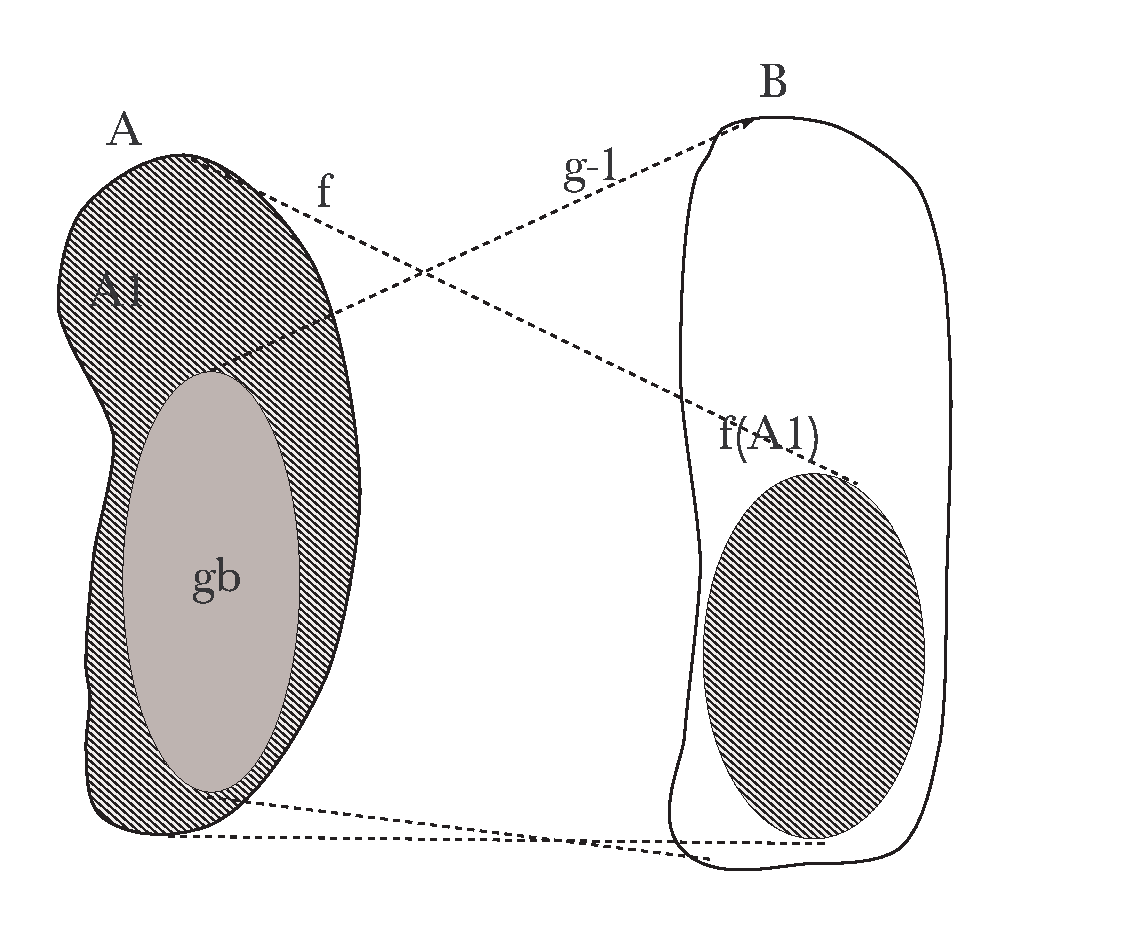
\includegraphics[height=10cm, width=10cm]{supfyg.eps}

\end{center}

 \caption{Las funciones $f$ y $g^{-1}$}\label{figura3}
\end{figure}

Una primera aproximaci\'on ser\'{\i}a intentar la construcci\'on
con $\tilde{A}=g(B)^c$. Seguramente as\'{\i} la funci\'on
$\tilde{f}$, ver ~\eqref{ftilde}, est\'a bien definida. La
funci\'on $\tilde{f}$ ser\'a suryectiva, pues $g^{-1}$ es
suryectiva de $g(B)$ en $B$. No obstante, con esa elecci\'on de
$\tilde{A}$, la funci\'on $\tilde{f}$ no es inyectiva, pues cada
elemento de $B_1$ es im\'agen, por esta $\tilde{f}$, de dos
elementos, uno en $A_1$ y otro en $g(B)$. De modo que esta
elecci\'on de $\tilde{A}$ todav\'{\i}a no nos sirve. Lo que vamos
a hacer ahora es agregarle a $\tilde{A}$ el conjunto de todos los
elementos de $g(B)$ tales que $g^{-1}$ los ``lleva'' a $B_1$. Este
conjunto es $A_2:=g(B_1)$. Definamos adem\'as $B_2:=f(A_2)$. Ahora
$\tilde{f}$ llevar\'a $A_1\cup A_2$ en $B_1\cup B_2$. Nos
preguntamos, ahora, si la elecci\'on $\tilde{A}:=A_1\cup A_2$ nos
servir\'a. Lamentablemente, la respuesta es
no\footnote{Podr\'{\i}a ser que si, si la funci\'on $f$ hubiera
sido biyectiva desde un principio, cosa que descartamos}. Al haber
``agrandado'' $\tilde{A}$ tambi\'en se nos agrand\'o el conjunto
de puntos en $B$ que son imagen de dos puntos, antes era el $B_1$,
ahora ``apareci\'o'' el $B_2$. De modo que continuamos el proceso,
es decir, definimos $A_3:=g(B_2)$, $B_3:=f(A_3)$ y as\'{\i}
sucesivamente, ver Figura \vref{figura4} . Nunca llegaremos, en
una cantidad finita de pasos, al conjunto $\tilde{A}$ con la
propiedad deseada, puesto que al cabo de $n$ pasos se nos genera
el conjunto $B_n$ donde las imagenes continuan superponiendos\'e.
?`Qu\'e haremos entonces?. Lo que se har\'a es seguir este proceso
indefinidamente, generando una sucesi\'on de conjuntos $A_n$ y
$B_n$, y luego definir:

\begin{equation}\label{defatilde}
\tilde{A}:=\bigcup_{n=1}^{\infty}A_n.
\end{equation}



\begin{figure}[h]

 \begin{center}

\psfrag{A}{$A$}

 \psfrag{B}{$B$}

 \psfrag{A1}{$A_1=A-g(B)$}
 \psfrag{A2}{$A_2=g(B_1)$}
 \psfrag{A3}{$ A_3=g(B_2)$}
\psfrag{B1}{$B_1=f(A_1)$}
 \psfrag{B2}{$B_2=f(A_2)$}
 \psfrag{B3}{$B_3=f(A_3)$}

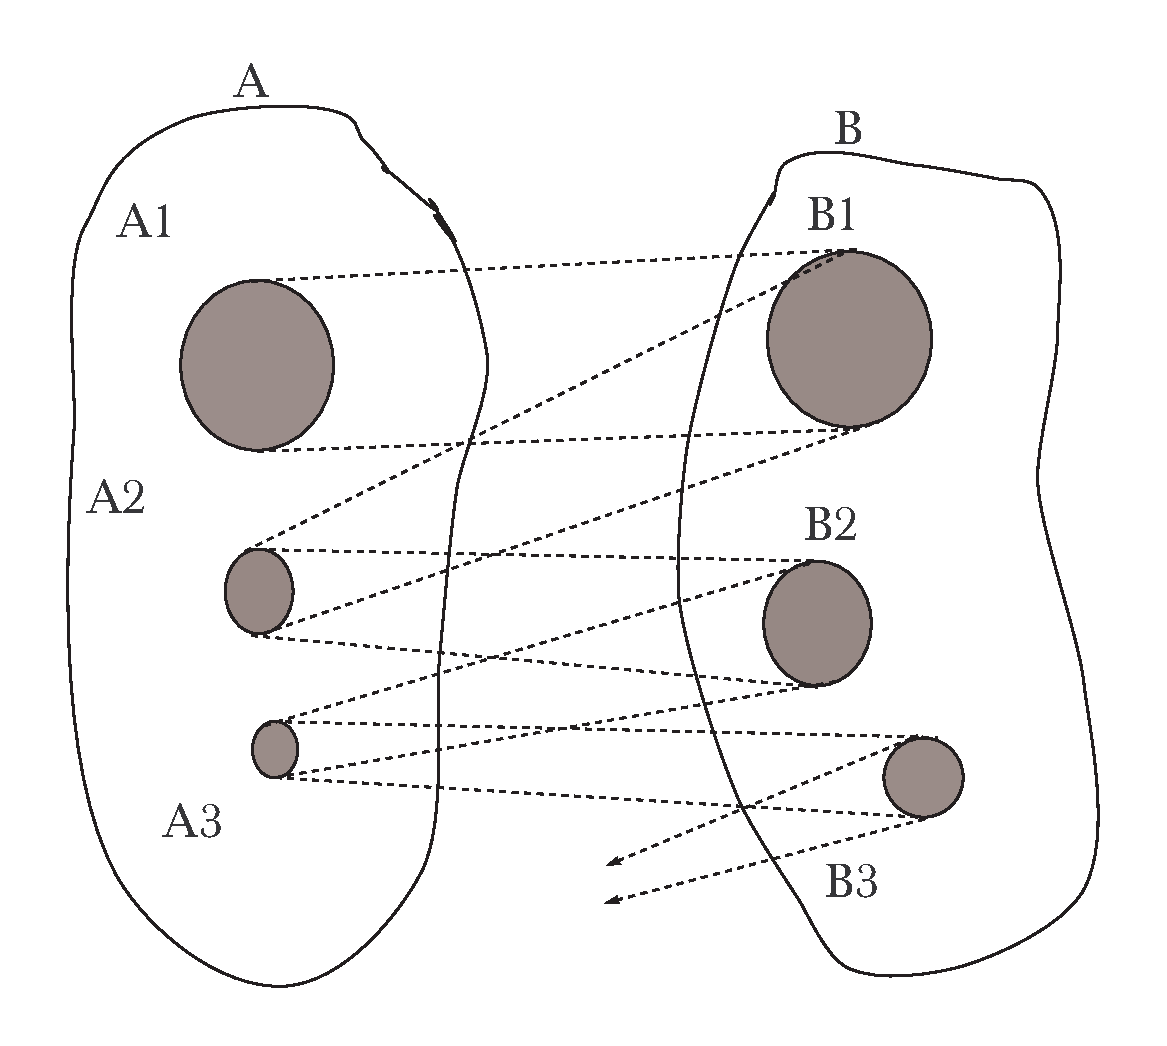
\includegraphics[height=10cm, width=10cm]{schber4.eps}

\end{center}

 \caption{Demostraci\'on del teorema de Schr\"oder-Berstein}\label{figura4}
\end{figure}

Intuitivamente, este conjunto deber\'{\i}a  funcionar, es decir no
hay m\'as superposici\'on de $f$ con $g^{-1}$. Esto es pues si
$a\in\tilde{A}$ entonces $a\in A_n$, para alg\'un $n$, y $f(a)\in
B_n$; eventualmente $f(a)$ podr\'{\i}a ser igual a alg\'un
$g^{-1}(a')$, pero $a'$ tendr\'{\i}a que estar en $A_{n+1}$ y por
consiguiente est\'a en $\tilde{A}$. Y as\'{\i}
$\tilde{f}(a')=f(a')$, y no $\tilde{f}(a')=g^{-1}(a')$, evitando
la superposici\'on de imagenes.

\vspace{10pt}
\begin{demo}\emph{Teorema \ref{scho-ber}} Estamos en condiciones de hacer la demostraci\'on propiamente
dicha del teorema. Hasta ahora solo tratamos de explicar la
demostraci\'on. Definimos inductivamente conjuntos $A_n$ y $B_n$
de la siguiente manera:

\[\left\{%
\begin{array}{ll}
    A_1=g(B)^c, & B_1=f(A_1) \\
    A_{n+1}=g(B_n), & B_{n+1}=f(A_{n+1}) \\
\end{array}%
\right..\]

Definamos $\tilde{A}$  como en ~\eqref{defatilde} y $\tilde{f}$
como en ~\eqref{ftilde}. Veamos que $\tilde{f}:A\longrightarrow B$
es biyectiva, empezando por la inyectividad.

Sean $a,a'\in A$ dos puntos cualesquiera tales que
$\tilde{f}(a)=\tilde{f}(a')$. Si $a$ y $a'$ est\'an
simultaneamente en $\tilde{A}$, o en $\tilde{A}^c$, tenemos que
$a=a'$ como consecuencia de que $f$, o $g^{-1}$, es inyectiva.
Consideremos, entonces, el caso $a\in\tilde{A}$ y $a'\notin
\tilde{A}$. Debemos llegar a una contradicci\'on pues estamos
suponiendo indirectamente que $a\neq a'$, por estar en conjuntos
disjuntos, y $\tilde{f}(a)=\tilde{f}(a')$. Tenemos que, para
alg\'un $n\in\nn$, $a\in A_n$; adem\'as, por la definici\'on de
$\tilde{f}$, tenemos que $f(a)=g^{-1}(a')$. Por consiguiente
$g(f(a))=a'$. Como $a\in A_n$, $f(a)\in B_n$ y $a'=g(f(a))\in
A_{n+1}$. Esto contradice que $a'\notin\tilde{A}$.

Veamos ahora la suryectividad. Sea $b\in B$ cualquier punto. Si
$b\in B_n$, para alg\'un $n$, como $B_n=f(A_n)$, ciertamente
existe un elemento $a\in A_n$ tal que $f(a)=b$. Ahora, por la
definici\'on de $\tilde{f}$, $\tilde{f}(a)=f(a)=b$. Supongamos,
pues, que $b$ no est\'a en ning\'un $B_n$. Como una afirmaci\'on
intermedia, probaremos que $g(b)$ no est\'a en ning\'un $A_n$.
Supongamos, por el contrario, que existe un $n$ tal que $g(b)\in
A_n$. Tiene que ser $n>1$, pues $A_1=g(B)^c$ y $g(b)\in g(B)$.
As\'{\i}, por su definici\'on  y como $n>1$, el conjunto $A_n$ es
igual a $g(B_{n-1})$. De modo que $g(b)\in g(B_{n-1})$. Esto
implica que existe un $b'\in B_{n-1}$ tal que $g(b)=g(b')$. Pero,
como $g$ es inyectiva $b=b'$ y, por ende, $b\in B_{n-1}$.
Contradiciendo esto que $b$ no estaba en ning\'un $B_n$. Probamos,
as\'{\i}, que $g(b)$ no est\'a en ning\'un $A_n$. Por lo tanto
$\tilde{f}(g(b))=g^{-1}(g(b))=b$. Vale decir $b=\tilde{f}(a)$ con
$a=g(b)$. Que era lo que quer\'{\i}amos probar.
\end{demo}

\section{Aplicaciones del Teorema de Schr\"oder-Berstein}

El teorema de Schr\"oder-Berstein es una herramienta potente para
probar coordinabilidad de conjuntos. En particular lo usaremos en
las cuestiones que a continuaci\'on exponemos. Hab\'{\i}amos visto
que $\rr\nsim\nn$. ?` Qu\'e ocurre con $\rr^2$, $\rr^3$,...?
?`Ser\'an estos conjuntos m\'as ``numerosos'' que $\rr$? Esto es:
?`Ser\'an no coordinables con $\rr$?. La respuesta a estas
preguntas es negativa, es decir $\rr^n\thicksim\rr$. Para ver esto
basta demostrar que $(0,1)^2\thicksim (0,1)$. El caso general es
consecuencia del caso $n=2$, usando inducci\'on, el Ejemplo
\vref{rcoord(0,1)} y el Ejercicio \vref{1.2}.

\begin{teorema} $(0,1)^2\thicksim (0,1)$.
\end{teorema}
\begin{demo} Observar que $(0,1)\precsim (0,1)^2$; podemos, para
demostrarlo, considerar la funci\'on inyectiva $f(x)=(x,1/2)$.

Veamos, ahora, que $(0,1)^2\precsim (0,1)$. Debemos construir una
funci\'on inyectiva $f:(0,1)^2\longrightarrow (0,1)$. Sea
$(x,y)\in (0,1)^2$. Consideremos las expresiones decimales
$x=0.x_1x_2...$ e $y=0.y_1y_2...$, donde $x_i$ e $y_i$ son enteros
entre 0 y 9, y no son todos 9 a partir de un momento en adelante.
Entonces escribimos:
\[f(x,y):=0.x_1y_1x_2y_2....\]
Es decir, $f$ intercala las expresiones decimales de $x$ e $y$.
Esta funci\'on es inyectiva, puesto que dos expresiones decimales
iguales tienen todos sus d\'{\i}gitos correspondientes iguales.
Esto concluye la demostraci\'on.
\end{demo}

Es bueno notar que la funci\'on $f$, definida en la demostraci\'on
anterior, no es suryectiva. Un n\'umero que no es imagen de
ning\'un par es $0.909090...$. ?`Por qu\'e ser\'a esto?

Por el Teorema \vref{teorcantor} tenemos que
$\nn\prec\mathcal{P}(\nn)$. Desmostramos, adem\'as, que $\nn\prec
\rr$. Nos preguntamos, ahora, que relaci\'on unir\'a
$\mathcal{P}(\nn)$ con $\rr$. Con el siguiente teorema probaremos
que aquellos conjuntos son coordinables.

\begin{teorema} $\mathcal{P}(\nn)\thicksim\rr$.
\end{teorema}
\begin{demo} Probaremos que $\mathcal{P}(\nn)\precsim\rr$ y despu\'es que
$\mathcal{P}(\nn)\succsim\rr$.

 Como $\mathcal{P}(\nn)\thicksim\mathbf{2}^{\nn}$ ( Ejercicio \vref{6}), y por el
 Ejercicio \vref{1.2} inciso 4, probaremos que $\mathcal{P}(\nn)\precsim\rr$ si podemos
 probar que $\mathbf{2}^{\nn}\precsim \rr$. Para este fin,
 consideremos la siguiente funci\'on:
 \[
    \begin{split}
          T:\mathbf{2}^{\nn}&\longrightarrow \rr\\
           f&\longmapsto 0.f(1)f(2)f(3)...\\
    \end{split}
 .\]
Esto es la funci\'on $f$ se aplica en un n\'umero cuya expansi\'on
decimal tiene solo ceros y unos. Esta funci\'on es inyectiva, pues
si
\[0.f(1)f(2)f(3)...=0.g(1)g(2)g(3)...\]
Entonces, por la unicidad de la expansi\'on
decimal\footnote{Recordemos que puede haber expresiones decimales
distintas que representan el mismo n\'umero, estas son las
expresiones que tienen todos nueves a partir de un momento en
adelante, como por ejemplo 1=0.999....No obstante este problema no
se nos presenta aqu\'{\i} pues la expresiones decimales que
consideramos tienen solo 0 y 1}, tenemos que $f(1)=g (1)$,
$f(2)=g(2)$,.... Por consiguiente las funciones son iguales. Lo
que prueba la inyectividad. De este modo demostramos que
$\mathbf{2}^{\nn}\precsim \rr$ y esto, por lo que explicamos
anteriormente, implica que $\mathcal{P}(\nn)\precsim \rr$

Ahora debemos ver que $\mathcal{P}(\nn)\succsim\rr$. Utilizando
los  incisos 1. y 4. del Ejercicios \vref{1.2}, vemos que es
suficiente probar que $\rr\precsim \mathcal{P}(\mathbb{Q})$. Para
hacer esto definimos la siguiente aplicaci\'on:
\[
   \begin{split}
        T:\rr &\longrightarrow \mathcal{P}(\mathbb{Q})\\
        r &\longmapsto \{q\in\mathbb{Q}:q<r\}
   \end{split}
.\]

Veamos que  la aplicaci\'on es inyectiva. Sean $r_1,r_2\in\rr$
n\'umeros reales distintos, supongamos $r_1<r_2$. Por la densidad
de $\mathbb{Q}$, existe un $q_0\in\mathbb{Q}$ tal que
$q_0\in(r_1,r_2)$. As\'{\i} $q_0\in\{q\in\mathbb{Q}:q<r_2\}$ y
$q_0\notin\{q\in\mathbb{Q}:q<r_1\}$. De modo que
\[\{q\in\mathbb{Q}:q<r_1\}\neq\{q\in\mathbb{Q}:q<r_2\}.\]
Es decir $T$ es inyectiva.
\end{demo}
Para finalizar demostraremos que
$\nn^{\nn}\thicksim\mathbf{2}^{\nn}$. Mas que el resultado en
s\'{\i}, vamos a resaltar su demostraci\'on, pues contiene una
idea interesante.

\begin{proposicion} $\nn^{\nn}\thicksim\mathbf{2}^{\nn}$.
\end{proposicion}

\begin{demo} Dado un conjunto $X$ cualquiera, podemos interpretar una
funci\'on $f\in X^{\nn}$ como una sucesi\'on de elementos de $X$,
a la que podemos disponer de la siguiente manera:
\begin{equation}\label{mensajes}
     f=(f(1),f(2),f(3),...).
\end{equation}
Si $X=\nn$ entonces la sucesi\'on ser\'a de n\'umeros naturales y
si $X=\mathbf{2}$ entonces la sucesi\'on ser\'a de ceros y unos.

Interpretemos el segundo miembro de ~\eqref{mensajes}  como una
palabra infinita. Si $X=\nn$, esta palabras se compone de
``letras'' que pueden ser cualquier n\'umero natural. Si
$X=\mathbf{2}$, esta ``palabra'' se escribe con solo dos
``letras'' el 0 y el 1. La pregunta es: ?`C\'omo podemos
``traducir'' una palabra escrita con un alfabeto de infitas
letras, a uno con solo dos?. La soluci\'on a esto es ingeniosa.
Sea $f\in\nn^{\nn}$, usaremos el signo 1 para denotar las comas en
la sucesi\'on $f$ y pondr\'emos tantos ceros como indiquen las
cantidades $f(j)$.


\[
  \begin{split}
         T\quad:\quad\nn^{\nn}\quad\quad &\longrightarrow\quad\quad\mathbf{2}^{\nn}\\
         f=(f(1),f(2),f(3),...)&\longmapsto
          (\underbrace{0,...,0}_{f(1)\,\,\text{ceros}},1,
          \underbrace{0,...,0}_{f(2)\,\,\text{ceros}},1,....)\\
 \end{split}
\]
Veamos que esta funci\'on es inyectiva. Sean $f,g\in\nn^{\nn}$,
con  $f\neq g$. Sea
\[j=\min\{i:f(i)\neq g(i)\}.\]
Tenemos que $f(i)=g(i)$ para $i<j$. Escribamos las dos sucesiones

\[   (\underbrace{0,...,0}_{f(1)\,\,\text{ceros}},1,
         ...,1,\underbrace{0,...,0}_{f(j-1)
          \,\,\text{ceros}},1, \underbrace{0,...,0}_{f(j)\,\,\text{ceros}},1,....)
\]
y
\[   (\underbrace{0,...,0}_{g(1)\,\,\text{ceros}},1,
         ...,1,\underbrace{0,...,0}_{g(j-1)
          \,\,\text{ceros}},1, \underbrace{0,...,0}_{g(j)\,\,\text{ceros}},1,....)
\]
Notar que los primeros $j-1$ grupos de ceros son iguales, pues
$f(i)=g(i)$ para $i<j$, por consiguiente los primeros $j-1$ unos
estan en la misma posici\'on en las dos sucesiones. Pero $f(j)\neq
g(j)$ y, por consiguiente, el grupo $j$-\'esimo de ceros debe
diferir en las dos sucesiones. Esto fuerza que si, por ejemplo,
$f(j)<g(j)$, entonces la sucesi\'on $f$ tendr\'a un uno donde la
$g$ tiene un cero.

As\'{\i} $T(f)\neq T(g)$ y la funci\'on es inyectiva. Esto prueba
que $\nn^{\nn}\precsim \mathbf{2}^{\nn}$. La otra desigualdad es
m\'as f\'acil de obtener pues
\[
  \begin{split}
      \mathbf{2}&\precsim \nn\quad\,\,\, \text{pues unos es finito y el
      otro no}\\
      \mathbf{2}^{\nn}&\precsim\nn^{\nn}\quad \text{por el
      Ejercicio \ref{potdelapot} }
  \end{split}
\]
\end{demo}

Existe una demostraci\'on m\'as sucinta de que
$\nn^{\nn}\precsim\mathbf{2}^{\nn}$. No la preferimos debido a que
no muestra una biyecci\'on, es una demostraci\'on indirecta. Ahora
la exponemos.
\[
  \begin{split}
       \nn &\precsim \mathbf{2}^{\nn}\quad\quad\,\text{Teorema de
       Cantor}\\
       \nn^{\nn} &\precsim (\mathbf{2}^{\nn})^{\nn}\quad\text{Ejercicio
       \ref{potdelapot}}\\
        \nn^{\nn} &\precsim \mathbf{2}^{\nn\times\nn}\quad\,\text{Ejercicio
       \ref{potdelapot}}\\
        \nn^{\nn} &\precsim \mathbf{2}^{\nn}\quad\quad\,\text{Proposici\'on  \ref{NxNesnum}}\\
        \nn^{\nn} &\precsim \mathbf{2}^{\nn}\quad\quad\,\text{Ejercicio
       \ref{1.2} inciso 3}.
  \end{split}
\]


\section{Ejercicios}


\begin{ejercicio}\label{propuniarb} Sea $f:A\longrightarrow B$ una funci\'on cualquiera.
Supongamos que $\{A_i\}_{i\in I}$ y $\{B_i\}_{i\in I}$ son
familias subindicadas de conjuntos, donde los $A_i$ y $B_i$ son
subconjuntos de $A$ y $B$ respectivamente. Demostrar las
siguientes propiedades:
\end{ejercicio}
\begin{itemize}
\item[1.] $\biggl(\bigcup_{i\in I}A_i\biggr)^c=\bigcap_{i\in
I}A_i^c$.
\item[2.]$\biggl(\bigcap_{i\in I}A_i\biggr)^c=\bigcup_{i\in
I}A_i^c$.
\item[3.] $f\biggl(\bigcup_{i\in I}A_i\biggr)=\bigcup_{i\in
I}f(A_i)$.
\item[4.]?`Qu\'e ocurre con $f\biggl(\bigcap_{i\in I}A_i\biggr)$?
\item[5.] $f^{-1}\biggl(\bigcup_{i\in I}B_i\biggr)=\bigcup_{i\in
I}f^{-1}(B_i)$.
\item[6.]$f^{-1}\biggl(\bigcap_{i\in I}B_i\biggr)=\bigcap_{i\in
I}f^{-1}(B_i)$.
\end{itemize}

\begin{ejercicio}\label{3} Demostrar las propiedades de la
Proposici\'on \vref{propfunc}
\end{ejercicio}
\begin{ejercicio}\label{1} Probar que $\thicksim$ es una
relaci\'on de equivalencia.
\end{ejercicio}
\begin{ejercicio}\label{1.2} Supongamos que $A\thicksim B$ y
$C\thicksim D$.
\begin{itemize}
\item[1.] Demostrar que $\mathcal{P}(A)\thicksim \mathcal{P}(B)$.
\item[2.] Demostrar que $A\times C\thicksim B\times D$.
\item[3.] Demostrar que $A^C\thicksim B^D$.
\item[4.] Si $A\precsim C$ entonces $B\precsim D$.
\end{itemize}
\end{ejercicio}
\begin{ejercicio}\label{potdelapot} Sean $A$, $B$ y $C$ conjuntos
no vacios. Demostrar que
\begin{itemize}
\item[1.] $\bigl(A^{B}\bigr)^C\thicksim A^{B\times C}$.
\item[2.] Si $A\precsim B$ entonces $A^C\precsim B^C$.
\end{itemize}
\end{ejercicio}

\begin{ejercicio}\label{1.5} Demostrar que un subconjunto de un conjunto
finito es finito.
\end{ejercicio}
\begin{ejercicio}\label{2} Demostrar que la funci\'on
$f:\nn\times\nn\longrightarrow\nn$ definida por:
\[f(j,k):=\frac{(j+k-1)(j+k)}{2}-j+1,\]
es una biyecci\'on.
\end{ejercicio}
\begin{ejercicio}\label{5} Demostrar, exhibiendo una biyecci\'on, que $(0,1)\thicksim [0,1]$
\end{ejercicio}
\begin{ejercicio}\label{6} Demostrar que el conjunto
$\mathcal{P}(\nn)$ es coordinable con el conjunto
$\mathbf{2}^{\nn}$, donde $\mathbf{n}=\{0,1,...,n-1\}$. Recordar
que, si $A$ y $B$ son conjuntos, $B^A:=\{f:f:A\longrightarrow
B\}$. De este modo $\mathbf{2}^{\nn}$ es el conjunto de funciones
$f:\nn\longrightarrow \{0,1\}$.
\end{ejercicio}

\begin{ejercicio}\label{8} Demostrar que, para cualquier conjunto
$A$, $\mathcal{P}(A)\thicksim\mathbf{2}^A$.
\end{ejercicio}
\begin{ejercicio}\label{infcoordconsub} Demostrar que son
equivalentes:
\begin{itemize}
     \item[1.] $A$ es infinito.
     \item[2.] $A$ es coordinable con un subconjunto propio, es
     decir: Existe $B\subset A$, con $B\neq A$, tal que
     $A\thicksim B$.
\end{itemize}
\end{ejercicio}
\begin{ejercicio} Demostrar que el conjunto formado por todos los
sub-\newline conjuntos de $\nn$ que son finitos, es numerable.
?`Qu\'e ocurrira con el conjunto de todos los subconjuntos
infinitos?
\end{ejercicio}
\begin{ejercicio} Sea $\{A_i\}_{i\in I}$ una familia de intervalos
de $\rr$. Suponer que los conjuntos en la familia son mutuamente
disjuntos, es decir: $A_i\cap A_j=\emptyset$ si $i\neq j$.
Demostrar que el conjunto $\{A_i:i\in I\}$ es a lo sumo numerable.
\end{ejercicio}
\begin{ejercicio} Recordemos que una funci\'on
$f:\rr\longrightarrow\rr$ se dice nodecre-\newline ciente, si para
todos $x,y\in\rr$, tales que $x<y$, se tiene que $f(x)\leq f(y)$.
Dada una funci\'on nodecreciente, demostrar que el conjunto de
todos los puntos de discontinuidad es a lo sumo numerable.
\textit{Ayuda}: Demostrar en primera instancia que los
l\'{\i}mites laterales:
\[
    \lim\limits_{x\rightarrow a^+}f(x)\quad\text{y}\quad \lim\limits_{x\rightarrow
    a^-}f(x)
\]
existen para todo $a\in\rr$. Luego aplicar el ejercicio anterior.
\end{ejercicio}
\begin{ejercicio} Demostrar que $\rr^{\nn}\thicksim\rr$.
\end{ejercicio}
\begin{ejercicio} Como aprendimos $\nn\thicksim\mathbb{Q}$, esto
significa que existe una aplicaci\'on biyectiva
$f:\nn\longrightarrow\mathbb{Q}$, que nos permite enumerar
$\mathbb{Q}$ como una suceci\'on $r_j:=f(j)$. Definimos la
aplicaci\'on:
\[\begin{split}
              T:C(\rr)&\longrightarrow \rr^{\nn}\\
              f        &\longmapsto T_f\\
\end{split}\]
donde
\[
  T_f(j):=f(r_j).
\]
\begin{itemize}
   \item [1.] Demostrar que $T$ es inyectiva. Por consiguiente
   $C(\rr)\precsim\rr^{\nn}$.
   \item[2.] Usando el inciso anterior, demostrar que
    $C(\rr)\thicksim\rr$, donde $C(\rr)$ es el conjunto
    de las funciones continuas de $\rr$ en si mismo.
\end{itemize}
\end{ejercicio}

%\documentclass[hyperref={colorlinks=true}]{beamer}
\documentclass[handout,hyperref={colorlinks=true}]{beamer}
\usepackage{pgfpages}
\pgfpagesuselayout{2 on 1}[a4paper,border shrink=5mm]

%\usepackage{color}
\definecolor{myblue}{rgb}{.8, .8, 1}
\usepackage{empheq}
\usepackage[spanish]{babel}
\usepackage[utf8x]{inputenc}
\usepackage{times}
\usepackage[T1]{fontenc}
\usepackage{amssymb,amsmath}
\usepackage{enumerate}
\usepackage{verbatim}
\usepackage{ esint }
%\usepackage{pst-all}
%\usepackage{pstricks-add}
\usepackage{array}
%\usepackage[T1]{fontenc}
\usepackage{animate}
%\usepackage{media9}
%% newcommand
\usepackage{xparse}

\newcommand{\com}{\mathbb{C}}
\newcommand{\dis}{\mathbb{D}}
\newcommand{\rr}{\mathbb{R}}

\newcommand{\oo}{\mathcal{O}}
\renewcommand{\emph}[1]{\textcolor[rgb]{1,0,0}{#1}}
\newcommand{\der}[2]{\frac{\partial #1}{\partial #2}}

\renewcommand{\epsilon}{\varepsilon}
\newcommand{\nl}{\onslide<+-> }

\newlength\mytemplen
\newsavebox\mytempbox

\makeatletter
\newcommand\mybluebox{%
    \@ifnextchar[%]
       {\@mybluebox}%
       {\@mybluebox[0pt]}}

\def\@mybluebox[#1]{%
    \@ifnextchar[%]
       {\@@mybluebox[#1]}%
       {\@@mybluebox[#1][0pt]}}

\def\@@mybluebox[#1][#2]#3{
    \sbox\mytempbox{#3}%
    \mytemplen\ht\mytempbox
    \advance\mytemplen #1\relax
    \ht\mytempbox\mytemplen
    \mytemplen\dp\mytempbox
    \advance\mytemplen #2\relax
    \dp\mytempbox\mytemplen
    \colorbox{myblue}{\hspace{1em}\usebox{\mytempbox}\hspace{1em}}}

\makeatother

 

\DeclareDocumentCommand\boxedeq{ m g }{%
    {\begin{empheq}[box={\mybluebox[2pt][2pt]}]{equation}% #1%
        \IfNoValueF {#2} {\label{#2}}%
       #1
       \end{empheq}
    }%
}



\DeclareMathOperator{\sen}{sen}
\DeclareMathOperator{\arcsen}{arcsen}
\newtheorem{teorema}{Teorema}[section]
\newtheorem{lema}[teorema]{Lema}
\newtheorem{corolario}[teorema]{Corolario}
\newtheorem{proposicion}[teorema]{Proposici\'on}
\newtheorem{definicion}[teorema]{Definici\'on}


\newenvironment{demo}{\noindent\emph{Dem.}}{$\square$ \newline\vspace{5pt}}



\mode<all>

{
  \usetheme{Boadilla}
  % oder ...
 
  \setbeamercovered{wolverine}
  % oder auch nicht
}





\title[Ecuaciones de primer órden, métodos de solución] % (optional, nur bei langen Titeln nötig)
{%
Ecuaciones de primer órden, métodos de solución
}



\author[] % (optional, nur bei vielen Autoren)
{Fernando Mazzone}

\institute[Depto de Matemática] % (optional, aber oft nötig)
{
 Depto de Matemática\\
Facultad de Ciencias Exactas Físico-Químicas y Naturales\\
Universidad Nacional de Río Cuarto}


\subject{Ecuaciones Diferenciales}

\begin{document}

\begin{frame}
  \maketitle
  \begin{center}
   
\includegraphics[scale=0.2]{unrc.jpg}
   \end{center}
\end{frame}















\section{Ecuaciones homogéneas}

\begin{frame}{Ecuaciones homogéneas}

\nl\begin{block}{Funciones homogéneas}
 Una función $F:\rr\times\rr\to\rr$ se dice homogénea de grado $\alpha$ si 
 \[f(rx,ry)=r^{\alpha}f(x,y).\]
\end{block}
\textbf{Ejemplos}
\begin{itemize}
                 \nl\item $f(x,y)=\tfrac{y}{x}$ es homogénea de grado $0$.
                \nl \item Más generalmente, cualquier función $f(x,y)$ que dependa sólo de $x/y$, esto es que se escriba de la forma $f(x,y)=g(y/x)$
                 es homogénea de grado  $0$. Así $f(x,y)=\tfrac{x-y}{x+y}$ es homogénea de grado $0$ pues $\tfrac{x-y}{x+y}= \tfrac{1-x/y}{1+x/y}$
                \nl \item $f(x,y)=\sum_{k=0}^na_kx^ky^{n-k}$ es homogénea de grado $n$.
\end{itemize}

\end{frame}

\begin{frame}{Ecuaciones homogéneas}

\nl\begin{block}{Resolviendo ecuaciones homogéneas}
 Una ecuación 
 \begin{equation}\label{ecua_prin}y'=f(x,y)\end{equation}
 tal que $f$ es homogénea de grado $0$ se llamará ecuación homogénea.
\end{block}

\nl\begin{block}{Resolviendo ecuaciones homogéneas}
 Si una ecuación del tipo \eqref{ecua_prin} es homogénea entonces se transforma en una ecuación separable mediante el cambio de variable dependiente $\boxed{z=y/x}$.
\end{block}


\end{frame}


\begin{frame}{Resolviendo ecuaciones homogéneas}

En efecto, para $x\neq 0$

\[f(x,y)=x^0f\left(1,\frac{y}{x}\right)=f(1,z)\]
y
\[y'=z'x+z\]
Como $y'=f(x,y)$ tenemos
\begin{equation}\label{cambio_hom}z'x+z=f(1,z)\Longrightarrow \frac{dz}{f(1,z)-z}=\frac{dx}{x}.\end{equation}
\end{frame}

\begin{frame}{Resolvieno ecuaciones homogéneas}
\textbf{Ejemplo} Resolver $y'=\frac{x+y}{x-y}$. 

La ecuación \eqref{cambio_hom} queda
\[ \begin{array}{c} \frac{dx}{x}=\frac{dz}{\frac{1+z}{1-z}-z}=\frac{(1-z)dz}{1+z^2}\\
 \Downarrow\\
\ln|x|+C=\arctan(x)-\frac{1}{2}\ln|1+z^2|
    \end{array}.
\]



\end{frame}

\section{Ecuaciones exactas}

\begin{frame}{Ecuaciones exactas}

\begin{block}{Definición}
\nl Dada una función $f$ de $n$ variables independientes $x_1,\ldots,x_n$ definimos su \href{http://es.wikipedia.org/wiki/Diferencial_de_una_función}{diferencial}
 por 
 \[df=\frac{\partial f}{\partial x_1}dx_1+\cdots +\frac{\partial f}{\partial x_n}dx_n.\]
\end{block}

\nl Es costumbre escribir las ecuaciones diferenciales   de la siguiente forma, supongamos  $f(x,y)=-M(x,y)/N(x,y)$
entonces
\[y'=-\frac{M(x,y)}{N(x,y)}\leftrightarrows M(x,y)dx+N(x,y)dy=0.\] 


\end{frame}

\begin{frame}{Ecuaciones exactas}
\nl Recordemos, dada $f:\rr\times\rr\to\rr$ la familia paramétrica de curvas
\[f(x,y)=c\]
satisface a ecuación diferencial

\[
 \frac{\partial f}{\partial x}+\frac{\partial f}{\partial y}y'=0\Longleftrightarrow \frac{\partial f}{\partial x}dx+\frac{\partial f}{\partial y}dy=0
 \Longleftrightarrow df=0.
\]
\nl El recíproco es tambien cierto, estos es una ecuación que se puede expresar como $df=0$  tiene soluciones dadas por la familia paramétrica de arriba. 

\nl Para que una ecuación cualquiera
\[M(x,y)dx+N(x,y)dy=0\]
Se pueda expresar como $df=0$ se debe cumplir que debe existir $f(x,y)$ tal que $M=\partial f/\partial x$ y $N=\partial f/\partial y$.
\end{frame}

\begin{frame}{Ecuaciones exactas}\label{camposconservativos}
\nl Vale decir el campo vectorial $(x,y)\mapsto (M(x,y),N(x,y))$ es un \href{http://es.wikipedia.org/wiki/Fuerza_conservativa}{campo 
gradiente o conservatico} con potencial $f$. No todo campo es un campo gradiente, recordemos

\nl \begin{block}{Caracterización de campos conservativos}Sea $\mathcal{O}$ abierto de $\rr^n$ y simplemente conexo. Son equivalentes
 \begin{enumerate}
  \item El campo $F:\mathcal{O}\to\rr^n$ es un gradiente.
  \item Si $C$ es un camino cerrado entonces
  \[\varointctrclockwise_C F\cdot d x=0.\]
  \item\label{item1} \[\frac{\partial F^i}{\partial x_j}=\frac{\partial F^j}{\partial x_i},\quad\text{ para }i,j=1,\ldots,n\]. 
 \end{enumerate}

\end{block}

\end{frame}

\begin{frame}{Ecuaciones exactas}
El item \ref{item1}  es particularmente simple de chequear. Una vez establecido con un campo es conservativo tendremos el problema de hallar el potencial $f$. 
Ilustremos esto con el campo $(x,y)\mapsto (M(x,y),N(x,y))$. Supongamos que $\mathcal{O}$ es abierto de $\rr^2$ y
\[\frac{\partial M}{\partial y}=\frac{\partial N}{\partial x},\quad\text{ para } (x,y)\in \mathcal{O}.\] 
En primer lugar debemos tener un campo escalar $f$ tal que
\[M=\frac{\partial f}{\partial x}\Rightarrow f=\int Mdx +C(y).\]
Ahora como $f_y=N$
\[N=\frac{\partial f}{\partial y}=\frac{\partial}{\partial y}\int Mdx +C'(y).\]

\end{frame}

\begin{frame}{Ecuaciones exactas}
\[C'(y)=N-\frac{\partial}{\partial y}\int Mdx .\]
\nl Para que esta ecuación tenga solución $N-\frac{\partial}{\partial y}\int Mdx$ debe ser sólo función de $y$. Pero la condición necesaria y suficiente para ello es 
\[\begin{split}0&=\frac{\partial}{\partial x}\left(N-\frac{\partial}{\partial y}\int Mdx\right)\\
&= \der{N}{x}-\frac{\partial^2}{\partial x\partial y}\int Mdx\\
&=\der{N}{x}-\frac{\partial^2}{\partial y\partial x}\int Mdx\\
&=\der{N}{x}-\der{M}{y}.
   \end{split}
\]
\end{frame}

\begin{frame}{Ecuaciones exactas}
\nl Pero estamos bajo ese supuesto, entonces
\boxedeq{C(y)=\int\left( N-\frac{\partial}{\partial y}\int Mdx \right)dy.}

\nl\textbf{Ejemplo} Resolver $e^ydx+(xe^y+2y)dy=0$. 

\nl\textbf{Solución} Aquí
\[M=e^y\quad\text{ y }N=xe^y+2y.\]
Así
\[\der{M}{y}=e^y=\der{N}{x}.\]
La ecuación es exacta. El potencial $f$ debe cumplir
\[f=\int e^ydx=xe^y+C(y)\]


\end{frame}


\begin{frame}{Ecuaciones exactas}
y
\[C(y)=\int\left( xe^y+2y -\frac{\partial}{\partial y} xe^y\right)dy= y^2\]
Tener en cuenta que la función potencial $f$ no es única, queda deerminada hasta una constante aditiva de integración que podemos elegir a gusto ya que 
debemos encontrar sólo un potencial. Entonces podemos tomar
\[f= xe^y+y^2.\]
La solución general de la ecuación estará dada por
\[xe^y+y^2=c,\quad c\in\rr.\]
Como no sabemos despejar $\boxed{y}$ de aquí dejamos indicada de esta manera la solución.

\end{frame}

\section{Factores integrantes}
\begin{frame}{Factores integrantes}
\nl Las ecuaciones exactas son raras, no obstante tenemos un recurso para llevar algunas ecuaciones no exactas a una equivalente y exacta.

\nl Supongamos que la ecuación
\[Mdx+Ndy=0\]
no es  exacta. La idea es econtrar una función $\mu(x,y)$ llamada 
\href{http://es.wikipedia.org/wiki/Ecuación_diferencial_exacta\#Factor_integrante.}{factor integrante} que haga que la ecuación
\[\mu\left(Mdx+Ndy\right)=0\]
si lo sea. Para ello se debe cumplir que
\begin{equation}\label{carac_factor}
  \der{\mu M}{y}=\der{\mu N}{x}\Longleftrightarrow \boxed{ \mu\der{M}{y}+\der{\mu}{y}M=\der{N}{x}\mu+N\der{\mu}{x}}.
\end{equation}
 
\end{frame}
 
 
\begin{frame}{Factores integrantes}
 \begin{block}{Observación}
  Toda ecuación
  \begin{equation}\label{ec_no_exa}Mdx+Ndy=0
   \end{equation}
  que tiene una solución general que se escribe
  \begin{equation}\label{sol_ec_no_exa}
   f(x,y)=c,  
  \end{equation}
  tiene, en teoría, un factor integrante. 
 \end{block}

 
 
 
\end{frame}

\begin{frame}{Factores integrantes}
Si derivamos \eqref{sol_ec_no_exa}
\[\der{f}{x}dx+\der{f}{y}dy=0.\]
De esta ecuación y \eqref{ec_no_exa} vemos que
\[-\frac{M}{N}=y'=-\frac{\partial f /\partial x}{\partial f/\partial y}\Longrightarrow \frac{ \partial f /\partial x}{M}=\frac{ \partial f/\partial y}{N}=:\mu(x,y)\]
Aquí hemos asumido $N\neq 0 \neq\der{f}{y}$. De la igualdad de arrriba se deduce que existe $\mu(x,y)$ con
\[\der{f}{x}=\mu M\quad\text{ y }\quad \der{f}{y}=\mu N.\]
Es decir $\mu$ es factor integrante.
\end{frame}

\begin{frame}{Factores integrantes}
La observación nos dice que parece razonable que siempre exista un factor integrante, pero no ayuda a hallarlo puesto que deberíamos conocer la solución general de la ecuación
para hacerlo. O deberíamos resolver la ecuación \eqref{carac_factor} que es una ecuación en derivadas parciales para $\mu$.

Hay que señalar que sólo necesitamos una solución de \eqref{carac_factor} y no su solución general. En la práctica se suele proceder a hacer alguna suposición
sobre $\mu$ que simplifique la expresión. Es común suponer que $\mu$ es sólo función de una de las variables. Si por ejemplo asumimos que $\mu=\mu(x)$ las ecuaciones 
\eqref{carac_factor} se escriben

\[\mu\der{M}{y}=\mu\der{N}{x}+N\mu'(x) \Longrightarrow\boxed{\frac{\mu'}{\mu}=\frac{\partial M/\partial y-\partial N/\partial x}{N}}\]
\end{frame}


\begin{frame}{Factores integrantes}
Para que esto funcione la función 

\[\frac{\partial M/\partial y-\partial N/\partial x}{N}\]

\emph{debe depender sólo de $x$}. Si eso ocurre y llamamos $h(x)$ a esa función vamos a tener que
\[\mu(x)=e^{\int h(x)dx}\]
es un factor integrante. Recordar que sólo necesitamos hallar uno, por ese motivo no consideramos constantes de integración. 
\end{frame}

\begin{frame}{Factores integrantes}
De manera similar, si la función
\[\frac{\partial M/\partial y-\partial N/\partial x}{-M}\]
depende sólo de $y$ y llamamos $h(y)$ a esa función tenemos que
\[\mu(y)=e^{\int h(y)dy}\]
es un factor integrante, que en este caso sólo depende de $y$.
\end{frame}

\begin{frame}{Factores integrantes}
\textbf{Ejemplo 1} $ydx+(x^2y-x)dy=0$.
Primero chequeemos la posible exactitud.
\[\der{M}{y}=1\text{ y } \der{N}{x}=2xy-1\Longrightarrow\text{no exacta}.\]
Ahora 
\[\frac{\partial M/\partial y-\partial N/\partial x}{N}=\frac{2-2xy}{x(xy-1)}=-\frac{2}{x}=:h(x).\]
El factor integrante es
\[\mu(x)=e^{\int h(x)dx}=e^{-2\ln |x|}=\frac{1}{x^2}.\]

\end{frame}


\begin{frame}{Exactitud, Otras Técnicas}

Veamos otra forma de trabajar para transformar ecuaciones no exactas en exactas. Aunque esta forma no es metódica, sino  que depende de la habilidad 
de quien la lleva adelante. Consiste en explotar la similitud de la ecuación diferencial con alguna expresión exacta conocida. Ilustremos esto con el ejemplo anterior 
$ydx+(x^2y-x)dy=0$. La ecuación equivale a
\[x^2ydy-(xdy-ydx)=0.\]
Ahora podemos notar que 
\[d\left(\frac{y}{x}\right)=\frac{xdy-ydx}{x^2}.\]
Lo que sugiere dividir por $x^2$ la ecuación.

\end{frame}

\begin{frame}{Exactitud, Otras Técnicas}

\[0=ydy-\frac{xdy-ydx}{x^2}=d\left(\frac{y^2}{2}\right)-d\left(\frac{y}{x}\right)=d\left(\frac{y^2}{2}-\frac{y}{x}\right).\]
La solución general es pues
\[\frac{y^2}{2}-\frac{y}{x}=c.\]

\end{frame}

\begin{frame}{Exactitud, Otras Técnicas}

Otras fórmulas para tener en cuenta que son exactas
%\begin{equation}
 \begin{align}
  d\left(\frac{x}{y}\right)&=\frac{ydx-xdy}{y^2}\quad\text{nada nuevo} \\
  d(xy)&=ydx+xdy\\
  d(x^2+y^2)&=2(xdx+ydy)\label{eq:exacta_mod2}\\
  d\left( \arctan\left(\frac{y}{x} \right) \right)&=\frac{ydx-xdy}{x^2+y^2}\quad\text{falla caracterización pag \ref{camposconservativos}!!!!}\nonumber\\
  d\left( \ln\left(\frac{y}{x} \right) \right)&=\frac{ydx-xdy}{xy}
  \end{align}
%\end{equation}


\end{frame}

\begin{frame}{Ejemplo, óptica}
\nl\begin{tabular}{m{5cm} m{4.5cm} }
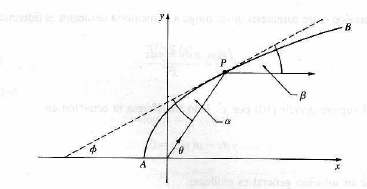
\includegraphics[scale=.4]{espejo.png} & \textbf{Problema} Hallar la forma del espejo curvo tal que el reflejo de todo haz de luz que viaja paralelo al eje $x$ con dirección
negativa repecto a este eje pasa por el $(0,0)$. \\
\end{tabular}
\nl \textbf{Ejercicio} Dejamos como ejercicio demostrar que un haz de luz que se refleja sobre un espejo lo hace de tal manera que los ángulos que se forman con los rayos 
de incidencia y refracción y la tangente al espejo en el punto de incidencia son iguales ( $\beta=\alpha$ en el dibujo). Para resolver esto hay que usar el principio
de mínimo tiempo de Fermat


\end{frame}


\begin{frame}{Ejemplo, óptica}
 \textbf{Solución.} Sea $(x,y)$ el punto de incidencia. Apelando a la geometría elemental, $\phi=\beta$ y $\theta=\alpha+\phi=2\beta$. Como $\tan\theta=\frac{y}{x}$
  y como
  \[\tan\theta =\tan 2\beta=\frac{2\tan\beta}{1-\tan^2\beta},\]
deducimos que
\[\frac{y}{x}=\frac{2 dy/dx}{1-(dy/dx)^2}.\]
Despejando
\[\frac{dy}{dx} =\frac{-x\pm\sqrt{x^2+y^2}}{y}.\]

\end{frame}


\begin{frame}{Ejemplo, óptica}
Podemos escribir la ecuación de este otro modo
\[xdx+ydy=\pm\sqrt{x^2+y^2}dx.\]
Tomando en cuenta \eqref{eq:exacta_mod2}
\[\pm\frac{x^2+y^2}{2\sqrt{x^2+y^2}}=dx.\]
Si $r=x^2+y^2$
\[dx=\pm\frac{dr}{2\sqrt{r}}=\pm d\sqrt{r}=\pm d\sqrt{x^2+y^2}\]
Las solución general es
\[\pm\sqrt{x^2+y^2}=x+c.\]
 


\end{frame}


\begin{frame}{Ejemplo, óptica}
 \begin{tabular}{m{4cm} m{5cm}}
 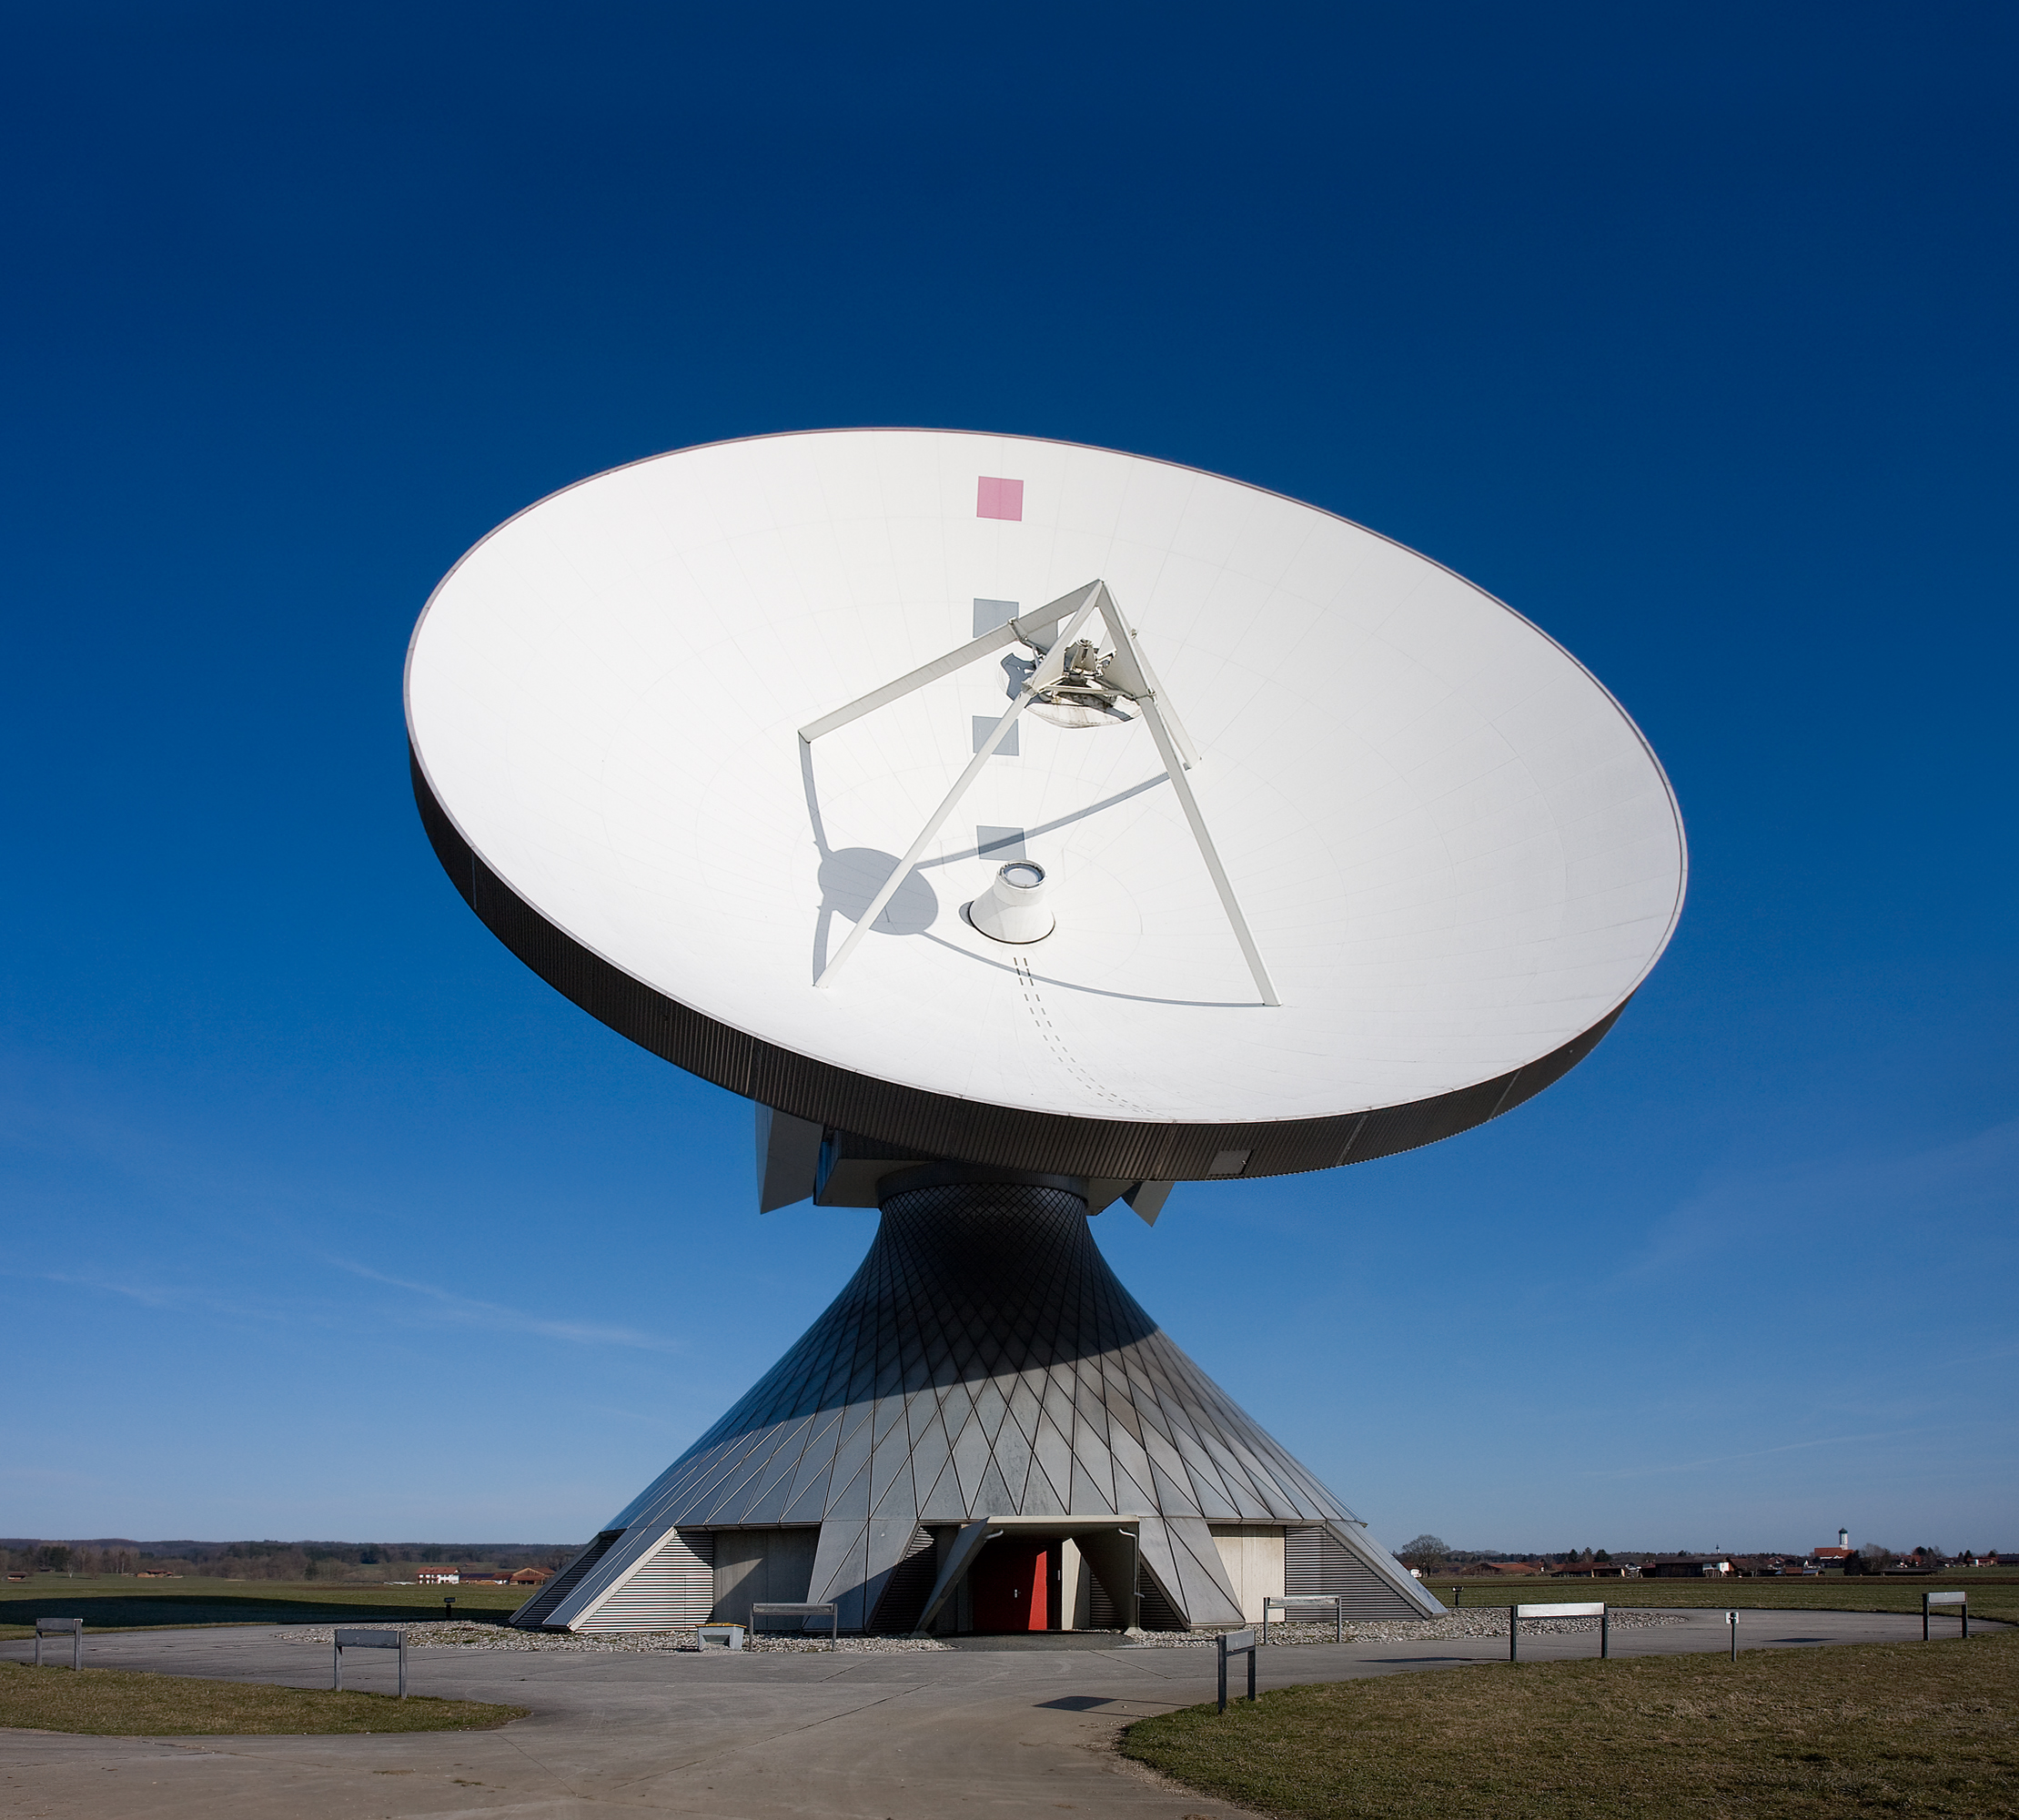
\includegraphics[scale=.15]{antena.jpg} & Elevando al cuadrado ambos miembros
\[y^2=2xc+c^2=2c\left(x+\frac{c}{2}\right)\]
Que es la familia de todas las parábolas con eje de simetría $x$, positivamente orientadas y con foco en $(0,0)$. \\
 \end{tabular}
 \end{frame}
\section{Ecuaciones Lineales}

\begin{frame}{Ecuaciones Lineales}
Se llama \href{http://es.wikipedia.org/wiki/Ecuación_diferencial_lineal}{ecuación diferencial lineal} a una ecuación que es lineal
respecto a   la/s variables
dependientes. La ecuación puede ser no lineal repecto a la variable independiente. 
La siguiente es la ecuación diferencial lineal general de primer orden
\begin{equation}\label{eq:lineal}y'+p(x)y=q(x).
\end{equation}
y la  de segundo orden
\[y''+p(x)y'+q(x)y=r(x).\]
Es costumbre introducir los operadores  $L_1[y]=y'+py$  y $ L_2[y]=y''+py'+qy$. 
Haciendo más precisa la definición, los operadores $L_1$ y $L_2$ son lineales, es decir, por ejemplo, $L_1[y_1+y_2]=L_1[y_1]+L_1[y_2]$. 
\end{frame}

\begin{frame}{Ecuaciones Lineales}
 Vamos a resolver la ecuación lineal de primer orden \eqref{eq:lineal}. Esto es sencillo pues la ecuación equivalente
 \begin{equation}\label{eq:lineal2}dy+(p(x)y-q(x))dx=0
  \end{equation}
tiene un factor integrante. En efecto como $M=p(x)y-q(x)$ y $N=1$. 
 \[\frac{\mu'}{\mu}=\frac{\partial M/\partial y-\partial N/\partial x}{N}=p(x).\]
 Entonces $\mu(x)=e^{\int pdx}$ es factor integrante. Luego si multiplicamos por $\mu$ en \eqref{eq:lineal2},  la expresión  es exacta. 
 \[e^{\int pdx}dy+p(x)e^{\int pdx}ydx=q(x)e^{\int pdx}dx.\]
\end{frame}

\begin{frame}{Ecuaciones Lineales}
Podemos identificar rápidamente, sin necesidad de hacer cálculos, el correspondiente potencial.
 \[d\left(e^{\int pdx}y\right)=d\left(\int q(x)e^{\int p} dx \right).\]
Integrando
\[e^{\int pdx}y=\int e^{\int pdx}q(x)dx+C.
 \]
 O
 \boxedeq{y=e^{-\int pdx}\left\{\int e^{\int pdx}q(x)dx+C\right\} }{SolGenLin}
 
 
 
 
\end{frame}


\begin{frame}{Ecuaciones Lineales}
\textbf{Ejemplo} Resolver $y'+y/x=3x$. 

\textbf{Solución.} En la práctica, para evitar recordar fórmulas, se suele repetir el procedimiento que llevo a la fórmula \eqref{SolGenLin}, ahora, dado la cercanía
de su derivación, vamos a usarla  de manera directa. La solución general es

\[\begin{split} y(x)&=e^{-\int\frac{1}{x}dx}\left\{\int e^{\int\frac{1}{x}dx}3xdx+C\right\}\\
   &=\frac{1}{|x|}\left\{\int |x| 3xdx+C\right\}\\
   &=x^2+\frac{C}{|x|}\\
   &=x^2+\frac{C}{x}\\
  \end{split}
\]
 
\end{frame}


\section{Reducción de orden}
\begin{frame}{Caso $F(x,y',y'')=0$}
Algunas ecuaciones de segundo orden
\boxedeq{F(x,y,y',y'')=0}{Gen2Or}
se pueden reducir a una de primer orden. Por ejemplo si $F$ no depende de $y$. Es decir la ecuación es
\boxedeq{F(x,y',y'')=0}
Aquí introducimos la nueva variable dependiente $\boxed{p=y'}$, que resuelve
\[F(x,p,p')=0.\]
Que es una ecuación de primer orden. Supuesto que la podemos resolver y encontrar una solución general para  $p$, tendremos
 

\end{frame}

\begin{frame}{Caso $F(x,y',y'')=0$}
 
\boxedeq{y=\int pdx+C}
Es la solución general de la ecuación de segundo orden.

\end{frame}

\begin{frame}{Caso $F(y,y',y'')=0$}\label{reduc_orden}
Si la ecuación general de segundo orden \eqref{Gen2Or} no depende de $x$, entonces nuevamente $\boxed{p=y'}$ como nueva variable depeniente
pero también usamos $\boxed{y}$ como nueva variable independiente. Como
\[y''=p'=\frac{dp}{dx}=\frac{dp}{dy}\frac{dy}{dx}=\frac{dp}{dy}p\]
La ecuación se reduce ala ecuación de primer orden
\boxedeq{F\left(y,p,\frac{dp}{dy}\right)=0}{RedOrdSinInd}

\end{frame}

\section{Ejemplos}

\begin{frame}{Velocidad de escape}\label{pag:vel_esc}

\begin{tabular}{m{4cm} m{5cm}}
 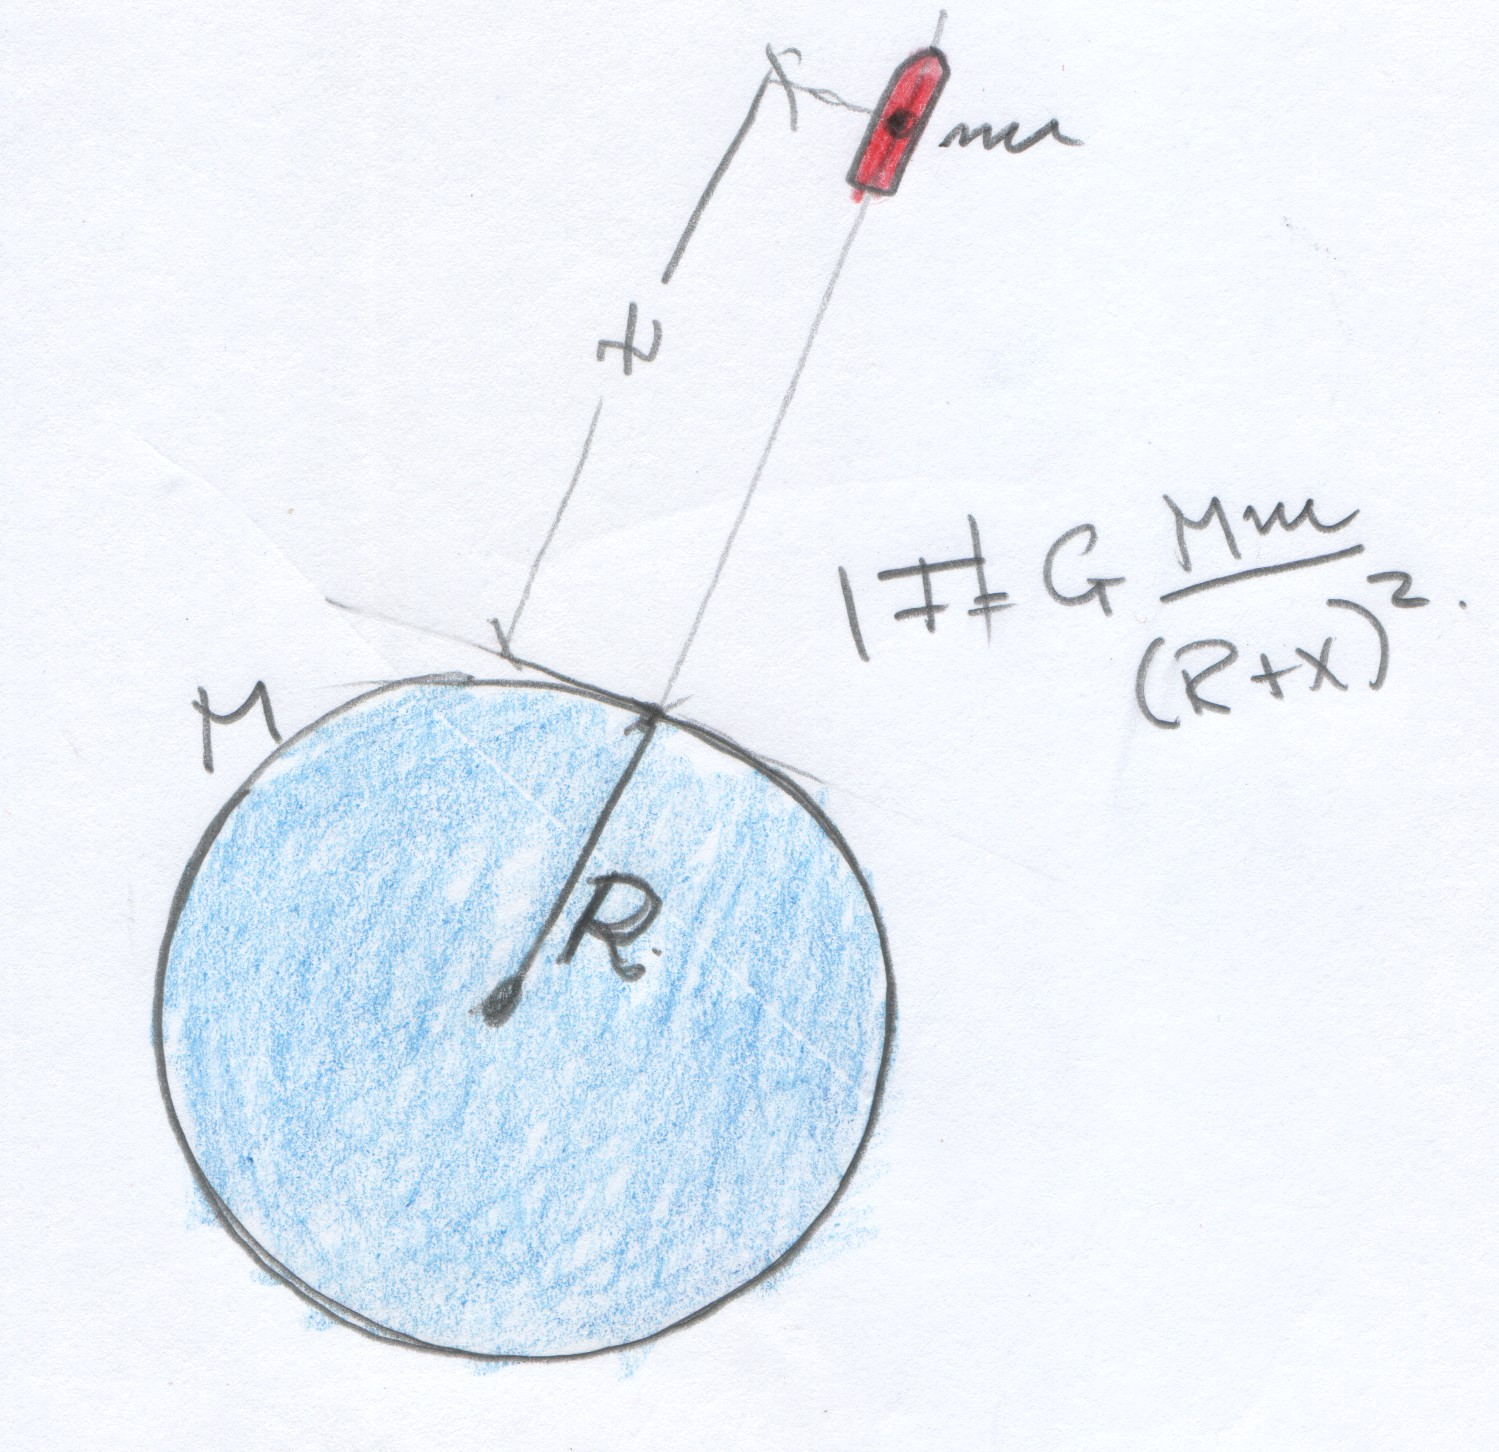
\includegraphics[scale=.075]{tiro_vertical.jpg}&\textbf{Problema.} Que velocidad hay que imprimirle a un proyectil que es lanzado verticalmente desde la superficie de la Tierra si nuestra pretensión
es que el proyectil se escape al infinito. La velocidad más chica con esta cualidad se llama 
\href{http://es.wikipedia.org/wiki/Velocidad_de_escape}{velocidad de escape}.\\
\end{tabular}
 


\end{frame}

\begin{frame}{Velocidad de escape}
\textbf{Solución.} Para resolver este problema hay que tomar en consideración la 
\href{http://es.wikipedia.org/wiki/Ley_de_gravitación_universal}{Ley de gravitación universal} de Newton. En la parte que nos interesa, esta Ley afirma
que el módulo de la fuerza de gravedad que se ejercen entre si dos cuerpos de masa $m_1$ y $m_2$ separados una distancia $r$ es proporcional al producto de las masas  
e inversamente proporcional al cuadrado de las distancia que los separa. Vale decir
\[|F|=G\frac{m_1m_2}{r^2},\]
donde $G$ es la constante de proporcionalidad.
Cuando los cuerpos no son puntos masa, sino cuerpos extendidos en el espacio, la distancia de separación hay que medirla entre los centros de masa de los cuerpos. 
\end{frame}


\begin{frame}{Velocidad de escape}
Hay que aclarar que usando el \href{https://docs.google.com/file/d/0B80iJ0HgObRRWll6MlJFSjFNMGc/edit}{Principio conservación energía mecánica} podemos resolver
el problema de una manera más simple. Incluso podemos ver que la suposición de que el tiro es vertical no es necesaria, es decir la velocidad e escape es la misma aunque
el tiro sea oblicuo. Discutiremos esa solución durante la clase. Lamentablemente (o no)  esta solución no usa ecuaciones diferenciales.
Vamos a dar una solución, quizás un poco más complicada, pero que invoca las técnicas 
discutidas.

 

\end{frame}

\begin{frame}{Velocidad de escape}
 

Supondremos a la Tierra una esfera de radio $R$, masa $M$ y su centro de masa en el centro de la esfera.   Al proyectil lo supondremos un punto masa 
con masa $m$ y su posición en el momento $t$, denotada $x=x(t)$, la mediremos sobre un eje vertical con origen en la superficie de la Tierra.  Todo como está indicado en la página \ref{pag:vel_esc}. 
Luego la distancia Tierra-proyectil será igual a $R+x$ donde $x$ es la posición del proyectil


\end{frame}

\begin{frame}{Velocidad de escape}
Utilizaremos la \href{http://es.wikipedia.org/wiki/Leyes_de_Newton\#Segunda_ley_de_Newton_o_ley_de_fuerza}{Segunda ley de Newton}, $F=ma$. Nos queda
\[mx''(t)=-\frac{GMm}{(R+x)^2}.\]
Es una ecuación de la forma
\[F(t,x,x',x'')=0.\]
Con variable dependiente $x$ e independiente $t$. Pero, en realidad no depende de $t$ y por consiguiente, como vimos, se puede convertir en una ecuación de primer orden
tomando como nuevas variables: 1) independiente $x$ 2) dependiente $v=x'$. En estas variables
\[\frac{d^2x}{dt^2}=\frac{dv}{dt}=\frac{dv}{dx}\frac{dx}{dt}=v\frac{dv}{dx}.\]


\end{frame}

\begin{frame}{Velocidad de escape}
Y la ecuación se convierte en
\[v\frac{dv}{dx}=-\frac{GM}{(R+x)^2}\Longrightarrow vdv+\frac{GM}{(R+x)^2}dx=0.\]
Que es una ecuación en variables separables y también es exacta. Usaremos la técnica discutida para 
ecuaciones exactas. 

Siempre las ecuaciones en variables separables son exactas pues se escriben de la forma
\[M(x)dx+N(y)dy=0\]
Tienen potencial
\[f=\int M(x)dx +\int N(y)dy\]


\end{frame}

\begin{frame}{Velocidad de escape}
Aplicando esto a nuestra ecuación
\begin{equation}\label{energia}
 \frac{v^2}{2}-\frac{GM}{(R+x)}=E=\text{cte}.
\end{equation}
  La igualdad anterior es precisamente 
 consecuencia directa del \href{https://docs.google.com/file/d/0B80iJ0HgObRRWll6MlJFSjFNMGc/edit}{Principio conservación energía mecánica}.
Sea $v_0$ la velocidad inicial para $t=0$. como $E$ es constante y $x=0$ en $t=0$ debe ser 
\begin{equation}\label{energia_cero}
 E=\frac{v_0^2}{2}-GM/R
\end{equation}
Como $v^2\geq 0$ y por \eqref{energia} y \eqref{energia_cero}.
\[-\frac{GM}{(R+x)}\leq\frac{v^2}{2}-\frac{GM}{(R+x)}=\frac{v_0}{2}-GM/R\]
 

\end{frame}

\begin{frame}{Velocidad de escape}
 
\onslide<+-> Queremos encontrar $v_0$ tal que $x\to\infty$. Luego tiene sentido tomar límite cuando $x\to\infty$ en la expresión anterior 
\[0\leq \frac{v_0^2}{2}-GM/R\]
\onslide<+-> De esto deducimos 

\begin{center}
 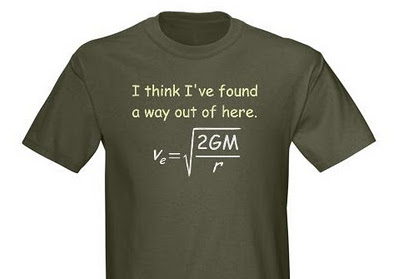
\includegraphics[scale=.4]{velocidad_escape.jpg}
\end{center}

\end{frame}


\begin{frame}{Curvas de persecución}
 
\textbf{Problema} Supongamos que un conejo se mueve sobre una 
línea recta con rapidez uniforme $a$ y de un punto por fuera de la recta parte un perro que lo 
persigue con rapidez uniforme $b$. Encontrar la trayectoria del perrro
 
\begin{center}
\animategraphics[controls, scale=.4]{15}{pursuit/pursuit-}{0}{40}
\end{center}

 
 
\textbf{Problema} Supongamos que un conejo se mueve sobre una 
línea recta con rapidez uniforme $a$ y de un punto por fuera de la recta parte un perro que lo 
persigue con rapidez uniforme $b$. Encontrar la trayectoria del perrro
 
\begin{center}
\animategraphics[controls, scale=.4]{15}{pursuit/pursuit-}{0}{40}
\end{center}
 
% \begin{tabular}{m{6cm} m{4cm}}
\textbf{Problema} Supongamos que un conejo se mueve sobre una 
línea recta con rapidez uniforme $a$ y de un punto por fuera de la recta parte un perro que lo persigue con rapidez uniforme $b$. Encontrar la trayectoria del perrro
\begin{center}
\animategraphics[controls, scale=.4]{15}{pursuit/pursuit-}{0}{40}
\end{center}
%\end{tabular}
 
 
\end{frame}

\begin{frame}{Curvas de persecución}
 \begin{tabular}{m{4.5cm} m{5cm}}
Supongamos que el perro parte del punto $(c,0)$, el conejo de $(0,0 )$ y la recta sobre la cual se mueve el conejo en dirección positiva  es el eje $y$. 
Vamos a suponer que la trayectoria del perro sigue la trayectoria tal que 
la tangente a su movimiento en un momento dado intersecta a la posición del conejo correspondiente a ese momento.
& 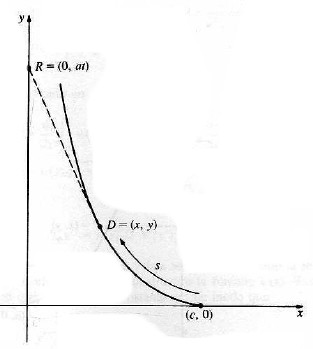
\includegraphics[scale=.4]{persecucion.jpg}
\end{tabular}
\end{frame}


\begin{frame}{Curvas de persecución}
Pasado un tiempo $t$, el conejo estará en el punto $(0,at)$ y el perro en un punto de su trayectoria que forma un arco de
 longitud $s=bt$ hasta el $(c,0)$. Ese punto, donde está el perro, lo denotaremos $(x,y)$. Como hemos supuesto que la tangente a la trayectoria del perro en $(x,y)$ pasa 
 por la posición del conejo $(0,at)$ se debe cumplir que
 \begin{equation}\label{eq:persec}\frac{dy}{dx}=\frac{y-at}{x}\Longrightarrow xy'-y=-at.\end{equation}
 En esta ecuación hay tres variables, $t$ , $x$ e $y$. No es muy claro cuales estamos usando como independiente y cuales depenientes. 
 Generalmente el tiempo $t$ es una variable  indepeniente, pero en la expresión de arriba aparece la derivada de $y$ respecto a $x$. 
\end{frame}

\begin{frame}{Curvas de persecución}
  Pareciese como 
 que estamos considerando   $y$ tanto función de $t$ como de $x$. La intuición nos dice que $y$ la puedo pensar tanto como función de una u otra.
 
 Tratemos de elinar $t$ de esa ecuación, de modo de tener una ecuación, una variable dependiente y una independiente, como el Dios de la matemática manda.
 
  No es razonable pensar que lograremos tener menos variables sin pagar algún precio, pues, como dice el dicho, 
 \href{http://es.answers.yahoo.com/question/index?qid=20081023132736AABMX0}{``Cuando la limosna es grande hasta el santo desconfía'' }. 
\end{frame}

\begin{frame}{Curvas de persecución}
 En este caso, el costo que pagaremos 
 es incrementar el orden de la ecuación. 
 Como hemos dado algunas técnicas de  resolver ecuaciones de orden dos quizás estemos en condiciones de pagar este precio.
 
Para eliminar $t$ de la ecuación derivamos $\eqref{eq:persec}$ respecto a $x$. Queda
\[xy''=-a\frac{dt}{dx}.\]
Como $ds/dt=b$ 
\[\frac{dt}{dx}=\frac{dt}{ds}\frac{ds}{dx}=-\frac{\sqrt{1+y'(x)^2}}{b}.\]
El signo menos aparece porque $s$ es decreciente con $x$ pues $s=\int_x^c\sqrt{1+y'^2}dx$.
 
\end{frame}

\begin{frame}{Curvas de persecución}
 Entonces 
 \boxedeq{xy''=\frac{a\sqrt{1+y'(x)^2}}{b}.}
 
Que es una ecuación que no contiene $y$. De modo que usando $p=y'$ como variable dependiente reducimos el orden de la ecuación. Nos queda
\[\frac{dp}{\sqrt{1+p^2}}=\frac{a}{b}\frac{dx}{x}.\]
Que es una ecuación en variable separables. Tomando la integral definida entre $c$ y $x$, y considerando que si $x=c$ entonces $p=0$, tenemos
\[\ln\left(p+\sqrt{1+p^2}\right)=\ln\left( \frac{x}{c}\right)^{\tfrac{a}{b}}.\]
 
 
\end{frame}

\begin{frame}{Curvas de persecución}

Si despejamos $p$ queda

\boxedeq{p=\frac{dy}{dx}=\frac{1}{2}\left[\left(\frac{x}{c}\right)^{a/b}-\left(\frac{c}{x}\right)^{a/b}\right].}

Vamos a dejar que la continuidad del análisis como ejercicio.
 
 
\end{frame}

\begin{frame}{Oscilador armónico}\label{resortito}

\begin{tabular}{m{6cm} m{2cm}}
 Un \href{http://es.wikipedia.org/wiki/Oscilador_armónico}{oscilador armónico} es el más simple de los sistemas físicos vibratorios. Podemos definirlo como un sistema
elástico que obedece a la \href{http://es.wikipedia.org/wiki/Ley_de_Hooke}{Ley de elasticidad de Hooke}, en honor a su descubridor 
\href{http://es.wikipedia.org/wiki/Robert_Hooke}{Robert Hooke} & 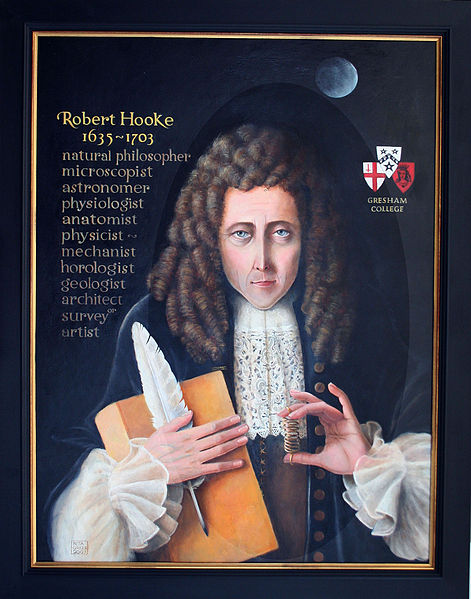
\includegraphics[scale=.15]{Hooke.JPG}\\
\end{tabular}

 
\end{frame}

\begin{frame}{Oscilador armónico}\label{resortito}

\begin{center}
\animategraphics[controls, scale=.4]{15}{resorte/resorte-}{0}{47}
\end{center}
 
\end{frame}

\begin{frame}{Oscilador armónico}
Suele citarse al \href{http://es.wikipedia.org/wiki/Resorte}{resorte} como un ejemplo familiar de oscilador armónico.

Esto debido a que, cuando las oscilaciones de un resorte son
pequeñas,  se satisface aproximadamente la Ley de elasticidad de  Hooke.

Esta ley  afirma que la fuerza que ejerce un resorte sobre una masa $m$ conectada a él por uno 
de sus extremos es proporcional en magnitud al desplazamiento
del resorte desde la posición de equilibrio.

Además la fuerza de elasticidad actúa en sentido opuesto al desplazamiento
 
\end{frame}


\begin{frame}{Oscilador armónico}
 Supongamos que tenemos un resorte, en unos de sus extremos fijado en una pared y unido a una masa $m$ por el otro extremo. Supongamos que no actúa otra fuerza 
 sobre la masa. Ver la animación de pag. \ref{resortito}.  Pongamos un eje de coordenadas en la dirección del movimiento, con origen en la posición de equilibrio 
 del resorte. Esta posición es el punto donde el resorte no ejerce fuerza. Supongamos que la dirección positiva es la dirección donde el resorte se expande. Denotemos 
 por $x(t)$ la posición de la masa en el momento $t$.  

\end{frame}
\begin{frame}{Oscilador armónico}
  Entonces según la Segunda Ley de Newton y la Ley de Elasticidad de Hooke, tenemos que
 
 \boxedeq{mx''(t)=-kx(t).}{eq:resorte}
 
La constante de proporcionalidad $k$ se llama \href{http://es.wikipedia.org/wiki/Rigidez}{constante elástica}. La ecuación \eqref{eq:resorte} se denomina la
ecuación del oscilador armónico o ecuación del resorte.

\end{frame}

\begin{frame}{Oscilador armónico}

La ecuación del oscilador armónico se escribe $0=f(t,x,x',x'')$, donde en $f(t,x,y,z)=kx+mz$ es independiente de $t$. Podemos intentar usar $x$ como variable 
independiente y $z=x'$ como dependiente. Como vimos en la página \ref{reduc_orden} $x''(t)=dz/dt=dz/dx z$. Así la ecuación queda
\[\begin{split}
   m\frac{dz}{dx}z=-kx &\Longrightarrow mzdz=-kxdx\Longrightarrow m\frac{z^2}{2}=-k\frac{x^2}{2}+C_1\\
   &\Longrightarrow z=\pm\sqrt{-\frac{k}{m}x^2+C_1}\\
   &\Longrightarrow x'(t)=\pm\sqrt{-\frac{k}{m}x^2+C_1}.\\
  \end{split}
\]


\end{frame}


\begin{frame}{Oscilador armónico}
Debe ser $C_1\geq 0$ de lo contrario el dominio de la función sería vacío. Nos queda una nueva ecuación para $x'$.
Esta ecuación es en variables separables
\[ \frac{dx}{\sqrt{-\frac{k}{m}x^2+C_1}}=dt.   
\]

\end{frame}

\begin{frame}{Oscilador armónico}
 Integrando
\[\begin{split}
   t+C_2 
   &=\int \frac{dx}{\sqrt{-\frac{k}{m}x^2+C_1}}\\
   &= \sqrt{\frac{1}{C_1}} \int \frac{dx}{\sqrt{-\frac{k}{C_1m}x^2+1}} \\  
   &= \sqrt{\frac{m}{k}} \int \frac{du}{\sqrt{1-u^2}}\quad \left(\text{haciendo } u=\sqrt{\frac{k}{C_1m}}x\right)\\ 
   &=\sqrt{\frac{m}{k}}\arcsen u.
  \end{split}
\]
\end{frame}

\begin{frame}{Oscilador armónico}
Entonces
\[\begin{split}
    x=\frac{C_1m}{k}u &=\frac{C_1m}{k}\sen \left(\sqrt{\frac{k}{m}}(t+C_2)\right)\\
    &=\boxed{C_3\sen \sqrt{\frac{k}{m}}t+C_4\cos \sqrt{\frac{k}{m}}t}.
  \end{split}
 \]

Que es la solución general de la ecuación del oscilador armónico. Como vemos el movimientoi es oscilatorio con frecuencia
\[\boxed{f=\sqrt{\frac{k}{m}} }.\]
En particular, no importan las condiciones iniciales, la frecuencia es siempre la misma. 

 
 

\end{frame}
\end{document}

%\documentclass{article}
%\documentclass[hyperref={colorlinks=true}]{beamer}
\documentclass[handout,hyperref={colorlinks=true}]{beamer}


%%%%%%%%%%%%%%%%%%%%%%%%%%%%%%Paquetes%%%%%%%%%%%%%%%%%%%%%%%%%%%%%%%%%%%%%%%%%%%%%%%5
%%%%%%%%%%%%%%%%%%%%%%%%%%%%%%%%%%%%%%%%%%%%%%%%%%%%%%%%%%%%%%%%%%%%%%%%%%%%%%%%%%%%%

\usepackage{pgfpages}
%\pgfpagesuselayout{2 on 1}[a4paper,border shrink=5mm]
\usepackage{empheq}
\usepackage[spanish]{babel}
\usepackage[utf8x]{inputenc}
\usepackage{times}
\usepackage[T1]{fontenc}
\usepackage{amssymb,amsmath}
\usepackage{enumerate}
\usepackage{verbatim}
\usepackage{ esint }
%\usepackage{pst-all}
%\usepackage{pstricks-add}
\usepackage{array}
%\usepackage[T1]{fontenc}
\usepackage{animate}
%\usepackage{media9}
\usepackage{xparse}
\usepackage{listings}
\usepackage{ wasysym }
\usepackage{sagetex}
\usepackage{hyperref}




%%%%%%%%%%%%%%%%%%%%%%%%%Configuracion listing
\lstdefinelanguage{Sage}[]{Python}
{morekeywords={False,sage,True},sensitive=true}
\lstset{
  frame=none,
  showtabs=False,
  showspaces=False,
  showstringspaces=False,
  commentstyle={\ttfamily\color{dgreencolor}},
  keywordstyle={\ttfamily\color{dbluecolor}\bfseries},
  stringstyle={\ttfamily\color{dgraycolor}\bfseries},
  language=Sage,
  basicstyle={\fontsize{8pt}{8pt}\ttfamily},
  aboveskip=.3em,
  belowskip=0.1em,
  numbers=none,
  numberstyle=\footnotesize
}


 


%%%%%%%%%%%%%%%%%%%%%%%%Colores
\definecolor{myblue}{rgb}{.8, .8, 1}
\definecolor{dblackcolor}{rgb}{0.0,0.0,0.0}
\definecolor{dbluecolor}{rgb}{0.01,0.02,0.7}
\definecolor{dgreencolor}{rgb}{0.2,0.4,0.0}
\definecolor{dgraycolor}{rgb}{0.30,0.3,0.30}
\newcommand{\dblue}{\color{dbluecolor}\bf}
\newcommand{\dred}{\color{dredcolor}\bf}
\newcommand{\dblack}{\color{dblackcolor}\bf}










%%%%%%%%%%%%%%%%%%%%%%%%%%Nuevos comandos entornos%%%%%%%%%%%%%%%%%%%%%%%%%%%%%%%%
%%%%%%%%%%%%%%%%%%%%%%%%%%%%%%%%%%%%%%%%%%%%%%%%%%%%%%%%%%%%%%%%%%%%%%%%
\newenvironment{demo}{\noindent\emph{Dem.}}{$\square$ \newline\vspace{5pt}}
\newcommand{\com}{\mathbb{C}}
\newcommand{\dis}{\mathbb{D}}
\newcommand{\rr}{\mathbb{R}}
\newcommand{\oo}{\mathcal{O}}
\renewcommand{\emph}[1]{\textcolor[rgb]{1,0,0}{#1}}
\newcommand{\der}[2]{\frac{\partial #1}{\partial #2}}
\renewcommand{\v}[1]{\overrightarrow{#1}}
\renewcommand{\epsilon}{\varepsilon}
\newlength\mytemplen
\newsavebox\mytempbox
\makeatletter
\newcommand\mybluebox{%
    \@ifnextchar[%]
       {\@mybluebox}%
       {\@mybluebox[0pt]}}

\def\@mybluebox[#1]{%
    \@ifnextchar[%]
       {\@@mybluebox[#1]}%
       {\@@mybluebox[#1][0pt]}}

\def\@@mybluebox[#1][#2]#3{
    \sbox\mytempbox{#3}%
    \mytemplen\ht\mytempbox
    \advance\mytemplen #1\relax
    \ht\mytempbox\mytemplen
    \mytemplen\dp\mytempbox
    \advance\mytemplen #2\relax
    \dp\mytempbox\mytemplen
    \colorbox{myblue}{\hspace{1em}\usebox{\mytempbox}\hspace{1em}}}

\makeatother
\DeclareDocumentCommand\boxedeq{ m g }{%
    {\begin{empheq}[box={\mybluebox[2pt][2pt]}]{equation}% #1%
        \IfNoValueF {#2} {\label{#2}}%
       #1
       \end{empheq}
    }%
}
\DeclareMathOperator{\atan2}{atan2}
\DeclareMathOperator{\sen}{sen}
\newtheorem{teorema}{Teorema}[section]
\newtheorem{lema}[teorema]{Lema}
\newtheorem{corolario}[teorema]{Corolario}
\newtheorem{proposicion}[teorema]{Proposici\'on}
\newtheorem{definicion}[teorema]{Definici\'on}
%%%%%%%%%%%%%%%%%%%%%%%%%%%%%%%%%%%%%%%%%%%%%%%%%%%%%%%%%%%%%%%%%%%%%%%%%%%%%%%%%%%%%%%%%%%%%%%%%%%%%%%%%%%




%%%%%%%%%%Para escibir en clase articulo o similar
% \usepackage{color}
% \newcommand{\nl}{ }
% \renewenvironment{frame}[1]{}{}
% \newcommand{\qed}{$\square$}
% %\newcommand{\defverbatim}{\def{#1}}
% \newenvironment{block}[1]{\textbf{#1}}{}
% \title{Ecuaciones lineales de segundo orden}
% \author{Fernando Mazzone}
% 




%%%%%%%%%%%%%%%%%%%%%%%Para clase beamer
\newcommand{\nl}{\onslide<+-> }
% \mode<all>
% {
%   \usetheme{Boadilla}
%   % oder ...
%  
%   \setbeamercovered{wolverine}
%   % oder auch nicht
% }


\mode<handout>{
  \usetheme{default}
  %\setbeamercolor{background canvas}{bg=black!5}
  \pgfpagesuselayout{4 on 1}[letterpaper,landscape,border shrink=2.5mm]
}

% \mode<all>{
%   \usetheme{default}
%   %\setbeamercolor{background canvas}{bg=black!5}
%   \pgfpagesuselayout{4 on 1}[letterpaper,landscape,border shrink=2.5mm]
% }

\title[Ecuaciones lineales de segundo orden] % (optional, nur bei langen Titeln nötig)
{%
 Ecuaciones lineales de segundo orden
}



\author[] % (optional, nur bei vielen Autoren)
{Fernando Mazzone}

\institute[Depto de Matemática] % (optional, aber oft nötig)
{
 Depto de Matemática\\
Facultad de Ciencias Exactas Físico-Químicas y Naturales\\
Universidad Nacional de Río Cuarto}


\subject{Ecuaciones Diferenciales}

%%%%%%%%%%%%%%%%%%%%%%%%%%%%%%%%%%%%%%%%%%%%%%%%%%%%%%%%%%%%%%%%%%%%%%%%%%%%%%%%%%%%%%




\begin{document}

\begin{frame}
  \maketitle
  \begin{center}
   
\includegraphics[scale=0.2]{imagenes/unrc.jpg}
   \end{center}
\end{frame}










\begin{frame}{Introducción}
\begin{block}{Ecuación lineal general de segundo orden}
\boxedeq{\frac{d^2y}{dx^2}+p(x)\frac{dy}{dx}+q(x)y=r(x),}{ec_2_gen}
donde $p,q,r$ son funciones definidas en un intervalo $I=(a,b)$ de $\rr$ con valores en $\rr$. 
\end{block}
Si $r\equiv 0$ se llama homogénea
\boxedeq{\frac{d^2y}{dx^2}+p(x)\frac{dy}{dx}+q(x)y=0,}{ec_2_gen_hom}
\end{frame}


\begin{frame}{Introducción}
\nl \begin{block}{Teorema de existencia y unicidad de soluciones}
 Supongamos $p,q,r$ continuas sobre $I$. Sean $x_0\in I$ e $y_0,y_1\in\rr$ dados. Entonces existe una única solución del PVI
 \[\left\{
 \begin{array}{l l l}
   \frac{d^2y}{dx^2}+&p(x)\frac{dy}{dx}+q(x)y=r(x),&x\in I\\
   y(x_0)&=y_0&\\
   y'(x_0)&=y^1_0&\\ 
  \end{array}\right.
\]


\end{block}
\nl \textbf{Demostración.} Más adelante.
\end{frame}


\section{Estructura del conjunto de soluciones}

\begin{frame}{Ecuaciones homogéneas}
\nl\begin{block}{Teorema}
 Si $y_1$ e $y_2$ son soluciones de \eqref{ec_2_gen_hom} y $c_1,c_2\in\rr$ entonces $c_1y_1+c_2y_2$ es solución. Vale decir, el conjunto de soluciones 
 es un espacio vectorial. En particular $y\equiv 0$ es una solución, a la que llameremos \emph{trivial}.

 

\end{block}

\nl\textbf{Demostración} 
 El operador 
 \[L[y]:=y''+py'+qy\]
es lineal, por consiguiente
$L[c_1y_1+c_2y_2]=c_1L[y_1]+c_2L[y_2]=0.$\qed
\end{frame}



\begin{frame}{Ecuaciones no homogéneas}
\nl\begin{block}{Teorema}
 Supongamos que $y_p$ es una solución particular de \eqref{ec_2_gen} y que $y_g=y_g(x,c_1,c_2)$ es una solución
 general de \eqref{ec_2_gen_hom}. Entonces $y=y_p+y_g$ es solución general de \eqref{ec_2_gen}.
\end{block}

\nl\textbf{Demostración} 
 El operador 
 \[L[y]:=y''+py'+qy\]
es lineal, por consiguiente
$L[y_g+y_p]=L[y_g]+L[y_p]=0+r=r.$
Recíprocamente supongamos $y$ solución de $L[y]=r$, entonces
$L[y-y_p]=L[y]-L[y_p]=r-r=0.$
Luego debe haber $c_1$ y $c_2$ con $y(x)-y_p(x)=y_g(x,c_1,c_2)$.\qed 
 
\end{frame}


\begin{frame}{Ecuaciones homogéneas}
\nl Volviendo a las ecuaciones homogéneas, supongamos que tenemos dos soluciones de \eqref{ec_2_gen_hom} $y_1$ e $y_2$. Entonces la expresión 
\begin{equation}\label{comb_lin}
   c_1y_1+c_2y_2,\quad c_1,c_2\in\rr
\end{equation}
es solución también. \nl Notar que en la expresión aparecen dos constantes y habíamos dicho que era de esperar que la solución general de una ecuación de orden 2 contuviese
precisamente dos constantes de integración. De modo que podemos conjeturar que \eqref{comb_lin} es solución general de \eqref{ec_2_gen_hom}. 

\nl Hay una situación especial, si, por ejemplo, $y_1=ky_2$, $k\in\rr$,entonces $c_1y_1+c_2y_2=(c_1k+c_2)y_2=cy_2$. Vale decir la combinación lineal \eqref{comb_lin}
termina siendo sólo combinación lineal de la función $y_2$ y por ende siendo esencialmente una expresión uniparamétrica.  
\end{frame}

\begin{frame}{Independencia lineal}
 
\begin{block}{Definición de independencia lineal}
 Un conjunto finito de funciones $\{y_1,\ldots,y_n\}$ se dirá linealmente independiente sobre un conjunto $I$, 
 si la única solución de $c_1y_1(t)+\cdots+c_ny_n(t)=0$, para $t\in I$, es $c_1=c_2=\cdots=c_n=0$.
\end{block}

\end{frame}

\begin{frame}{Independencia lineal}
 
\begin{block}{Definición wronskiano}

Dadas $n$ fuciones  $\{y_1,\ldots,y_n\}$ con dominio $I$ el wronskiano $W(x)=W(y_1,y_2,\ldots,y_n)(x)$ de estas funciones en un punto $x\in I$ se define por
\boxedeq{W(x)=\det\begin{pmatrix}
                                  y_1(x) & y_2(x) & \cdots &y_n(x)\\
                                  y_1'(x) & y_2'(x) & \cdots &y_n'(x)\\
                                  \vdots & \vdots &\ddots& \vdots\\
                                  y_1^{(n-1)}(x) & y_2^{(n-1)}(x) & \cdots &y_n^{(n-1)}(x)\\
                               \end{pmatrix}}{wronskiano}
\end{block}
\end{frame}


\begin{frame}{Independencia lineal}
\nl\begin{block}{Lema. Propiedades Wronskiano I}
Sea $\{y_1,\ldots,y_n\}$ un conjunto de $n$ funciones. Si existe un $x_0\in I$ con $W(x_0)\neq 0$ entonces   $\{y_1,\ldots,y_n\}$ son
linealmente independientes
\end{block}

\nl\textbf{Demostración.} Supongamos que $c_1y_1+\cdots+c_ny_n\equiv 0$. Derivando $n-1$ veces esta igualdad y evaluando el resultado en $x_0$ obtenemos
\[
 \begin{split}
    c_1y_1(x_0)+\cdots+c_ny_n(x_0)&=0\\
    c_1y_1'(x_0)+\cdots+c_ny'_n(x_0)&=0\\
    \vdots \quad& \quad\vdots\\
    c_1y_1^{(n-1)}(x_0)+\cdots+c_ny^{(n-1)}_n(x_0)&=0\\
 \end{split}
\]


\end{frame}

\begin{frame}{Independencia lineal}
 Las igualdades anteriores dicen que el vector $(c_1,\ldots,c_n)^t$ pertenece al nucleo de la matriz 
\[
\begin{pmatrix}
                                  y_1(x_0) & y_2(x_0) & \cdots &y_n(x_0)\\
                                  y_1'(x_0) & y_2'(x_0) & \cdots &y_n'(x_0)\\
                                  \vdots & \vdots &\ddots& \vdots\\
                                  y_1^{(n-1)}(x_0) & y_2^{(n-1)}(x_0) & \cdots &y_n^{(n-1)}(x_0)\\
                               \end{pmatrix}
\]
Como por hipótesis la matríz es no singular, debe ocurrir que $c_1=c_2=\cdots c_n=0$. \qed

\end{frame}
\begin{frame}{Fórmula de Abel}
\begin{block}{Teorema. Propiedades wronskiano II}
Supongamos que  $y_1$ e $y_2$  son solución de 
\begin{equation}\label{eq2orden}\frac{d^2y}{dx^2}+p(x)\frac{dy}{dx}+q(x)y=0,\quad x\in I=(a,b)\end{equation}
 Entonces existe $c\in\rr$ que satisface
\boxedeq{W(y_1,y_2)(x)=ce^{-\int p dx}.}{formu_abel}
Esta expresión  se denomina \href{http://en.wikipedia.org/wiki/Abel's_identity}{fórmula de Abel}. En particular vale que
\[\exists x_0\in I: W(x_0)\neq 0 \Longleftrightarrow \forall x\in I: W(x)\neq 0 .\]
\end{block}
\end{frame}


\begin{frame}{Demostración fórmula Abel}
\textbf{Demostración.} Tenemos que 
\[W(x)=y_1(x)y_2'(x)-y_1'(x)y_2(x).\]
Derivando y usando \eqref{eq2orden}
\[\begin{split}W'(x)&=y_1y_2''-y_1y_2''\\
   &=y_1(-py_2'-qy_2)-y_2(-py_1'-qy_1)\\
   &=-pW.
  \end{split}
\]
Vale decir $W$ resuelve la ecuación $W'=-pW$ la cual es facilmente resoluble, mostrando su resolución que se satisface \eqref{formu_abel}\qed 


\end{frame}
 
 
\begin{frame}{Independencia y wronskiano}
\nl\begin{block}{Propiedades wronskiano III}
 Sean $y_1$ e $y_2$ soluciones de \eqref{eq2orden}. Entonces son equivalentes
 \begin{enumerate}
  \item\label{item1} $y_1$ e $y_2$ son linealmente indepenientes en $I$. 
  \item\label{item2} $W(y_1,y_2)(x)\neq 0$ para todo $x\in I$.
 \end{enumerate}
\end{block}
\nl\textbf{Demostración.}  Que \ref{item2} implica \ref{item1} es consecuencia de la propiedad del wronskiano I. 
Veamos que \ref{item1} implica \ref{item2}. Supongamos que exista un $x_0$ con $W(x_0)=0$. Esto quiere decir  que una de las columnas
de la matríz wronskiana en $x_0$ es múltiplo de la otra. Supongamos que $y_2(x_0)=ky_1(x_0)$ e $y'_2(x_0)=ky'_1(x_0)$. Esto quiere decir que $y_2$ y $ky_1$
resuelven el mismo pvi. Por lo tanto $y_2(x)=ky_1(x)$ para todo $x$. Lo que nos dice lo contrario de \ref{item1}\qed

\end{frame} 
 
\begin{frame}{Estructura soluciones ecuaciones homogéneas}
\begin{block}{Teorema, estructura del conjunto de soluciones ecuación lineal de segundo orden homogénea}
Si $y_1$ e $y_2$ son soluciones linealmente independientes de 
\[\frac{d^2y}{dx^2}+p(x)\frac{dy}{dx}+q(x)y=0,\quad x\in I=(a,b)\]
entonces
\boxedeq{ y(x,c_1,c_2)=c_1y_1+c_2y_2}{comb_lin2}
es solución general.
\end{block}

\end{frame}

\begin{frame}{Estructura soluciones ecuaciones homogéneas}
\textbf{Demostración.} Que la expresión \eqref{comb_lin2} es solución ya lo hemos dicho.   Restaría ver que cualquier solución se escribe como en \eqref{comb_lin2}. 
Sea $y$ cualquier solución y $x_0\in I$. La matriz wronskiana
\[\begin{pmatrix}
   y_1(x_0)  & y_2(x_0)\\
   y'_1(x_0)  & y'_2(x_0)\\   
  \end{pmatrix}
\]
Es no singular dado que el determinante es no nulo. Por este motivo el sistema
\[ \begin{split}
  c_1 y_1(x_0) + c_2y_2(x_0) &=y(x_0)\\
   c_1y'_1(x_0)  + c_2y'_2(x_0) &=y'(x_0)\\
  \end{split}
\]
tiene solución para $c_1$ y $c_2$. 
\end{frame}


\begin{frame}{Estructura soluciones ecuaciones homogéneas}
De este modo vemos que la función  $c_1y_1+c_2y_2$ resuelve el PVI

 \[\left\{
 \begin{array}{l l l}
   \frac{d^2z}{dx^2}+&p(x)\frac{dz}{dx}+q(x)z=0,&x\in I\\
   z(x_0)&=y(x_0)&\\
   z'(x_0)&=y'(x_0)&\\ 
  \end{array}.\right.
\]
Evidentemente $y$ es solución también, por el Teorema de Existencia y Unicidad vemos que $y=c_1y_1+c_2y_2$ \qed
\end{frame}

\section{Reducción de orden}
\begin{frame}{Reduccción de orden}
\nl Como conclusión de los anterior, vemos que si queremos resolver \eqref{eq2orden} debemos conseguir  dos soluciones linealmente independientes.

\nl Suponiendo que ya contamos con una solución no trivial vamos a describir un método 
  que posibilita  encontrar otra solución $y_2$ linealmente independiente de $y_1$. 
  
\nl El método consiste en proponer que $y_2$ se escribe

\[\boxed{y_2(x)=v(x)y_1(x)}.\]


\end{frame}


\begin{frame}{Reduccción de orden}
Luego
\[
 \begin{split}
    0&=y_2''+py_2'+qy_2\\
    &=y_1v''+2v'y_1'+vy_1''+pv'y_1+pvy_1'+qvy_1\\
    &=y_1 v''+(2y_1'+py_1)v'+v(y_1''+py_1'+qy_1)\\
    &=y_1 v''+(2y_1'+py_1)v'
 \end{split}
\]
La fórmula anterior es nuevamente una ecuación de segundo orden para $v$, 
pero en este caso afortunadamente contamos con herramientas para resolverla puesto que se trata de una ecuación donde la 
variable dependiente $v$ no aparece explícitamente, sino que aparecen sus derivadas $v'$ y $v''$. Hay que intentar la sustitución $w=v'$


\end{frame}
 
 
\begin{frame}{Reduccción de orden}
Luego
\[
 y_1w''+(2y_1'+py_1)w=0
\]
Recordar que $y_1$ la asumimos conocida y que $p$ es obviamente conocida, así $2y_1'+py_1$ es una funcióon conocida. La ecuación es una ecuación lineal homogénea de primer orden. 
Usando la fórmula para resolver este tipo de ecuación dada en nuestra 
\href{https://github.com/fdmazzone/Material-Ecuaciones-Diferenciales/blob/master/uni2.pdf?raw=true}{presentación anterior}, obtenemos
\[w(x)=Ce^{-\int \frac{y_1'}{y_1}+p dx}=Ce^{-2\ln|y_1|}e^{-\int p dx}=C\frac{1}{y_1^2}e^{-\int p dx} \]
Es suficiente encontrar sólo una función $v$, de allí podemos tomar $C=1$. 
\boxedeq{w(x)= \frac{1}{y_1^2}e^{-\int p dx}\Longrightarrow v(x)= \int \frac{1}{y_1^2}e^{-\int p dx}dx }{reduc_orden}



\end{frame} 

\begin{frame}{Reduccción de orden}
\nl Otra manera de testear la independencia lineal de dos funciones $y_1$ e $y_2$ es notar que si fueran linealmente dependientes e $y_1\neq 0$ 
en un conjunto $J\subset I$ entonces $y_2/y_1$
sería constante.  
\nl Luego uno chequearía independencia si comprobase que $y_2/y_1$ no es constante en algún subdominio $J\subset I$. 

\nl En el caso anterior $y_2/y_1=v$, luego 
deberíamos tener $v$ no constante sobre algún subconjunto $J$. Pero $v$ constante implicaría $y_1^{-2}e^{-\int pdx}=0$ y esto claramente no ocurre. De modo que por el
método anterior encontramos dos soluciones independientes.   





\end{frame} 


 \section{Ecuaciones homogéneas con coeficientes constantes}
\begin{frame}{Ecuaciones homogéneas con coeficientes constantes}
 
 Consideramos la ecuación
 
 \boxedeq{y''+py'+qy=0,\quad p,q\in\rr}\label{2orden_coef_ctes}
    
 Propongamos una solución de la forma 
 \[\boxed{y(x)=e^{\lambda x},\quad \lambda\in\mathbb{C}}\]
 Reemplazando en la ecuación
 \[(\lambda^2+\lambda p+q)e^{\lambda x}=0.\]
Se debe satisfacer la llamada \emph{ecuación característica}
\boxedeq{\lambda^2+p\lambda+q=0}{ecua_carac} 
\end{frame}

\begin{frame}{Ecuaciones homogéneas con coeficientes constantes}
Tenemos tres casos acorde al valor de $\Delta:=p^2-4c$

\nl 1)\textbf{$\boxed{\Delta=p^2-4c>0}$, raices reales distintas $\lambda_1$, $\lambda_2$}. Este es el caso más sencillo de todos, obtenemos las soluciones
\[y_1(x)=e^{\lambda_1 x}\quad\text{y}\quad y_2(x)=e^{\lambda_2 x}.\]
Para chequear la independencia
\[\frac{y_2}{y_1}=e^{(\lambda_2-\lambda_1)x}\neq\text{cte}.\]
Luego 
\boxedeq{y(x,c_2,c_2)=c_1e^{\lambda_1 x}+c_2e^{\lambda_2 x}.}{sol_gen1}
es solución general
\end{frame}

\begin{frame}{Ecuaciones homogéneas con coeficientes constantes}
2) \textbf{$\boxed{\Delta=p^2-4c<0}$, raices complejas conjugadas $\lambda_1=\mu+i\nu$, $\lambda_2=\mu-i\nu$, $\mu,\nu\in\rr$}.

Proponemos una solución de la forma
\[
 y(x)=e^{\mu x}v(x)
\]

Hagamos los cálculos con SAGE
 



\end{frame}

\defverbatim[colored]\lstI{ 
\begin{lstlisting}
sage: x,p,q=var('x,p,q')
sage: y=function('y',x)
sage: v=function('v',x)
sage: y=exp(-p/2*x)*v
sage: ecua=y.diff(x,2)+p*y.diff(x)+q*y==0
sage: ecuav=(ecua/exp(-p/2*x)).simplify_full()
sage: ecuav
-1/4*(p^2 - 4*q)*v(x) + D[0, 0](v)(x) == 0


\end{lstlisting}
 }




\begin{frame}{Ecuaciones homogéneas con coeficientes constantes}
\lstI

Vale decir  que $v$ resuelve
\[-\frac{1}{4} \, {\left(p^{2} - 4 \, q\right)} v\left(x\right) + v''(x) = 0.\]

Como $-\frac{1}{4}(p^2-4q)>0$,  estamos en presencia de la ecuación del oscilador armónico. 
\end{frame}




\begin{frame}{Ecuaciones homogéneas con coeficientes constantes}
 


Recordar que si $\nu=\sqrt{\frac{|p^2-4q|}{4}}$, la solución general 
para $v$ es
\[v(x)=C_1\cos \nu x +C_2\sen \nu x,\]
y de allí
\boxedeq{y(x)=e^{\mu x}\left\{C_1\cos \nu x +C_2\sen \nu x\right\}}{sol_gen_2caso}



\end{frame}


\begin{frame}{Ecuaciones homogéneas con coeficientes constantes}
 
\begin{tabular}{c c c}
 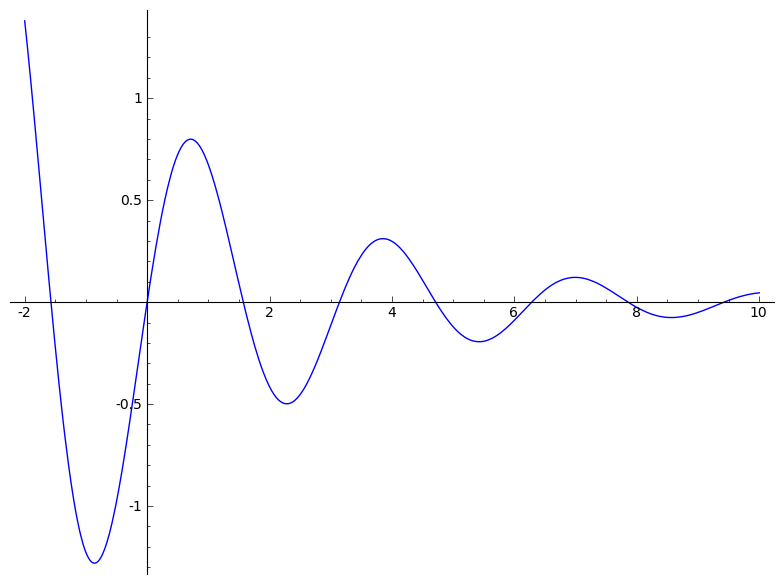
\includegraphics[scale=.1]{imagenes/mu_neg.png} & 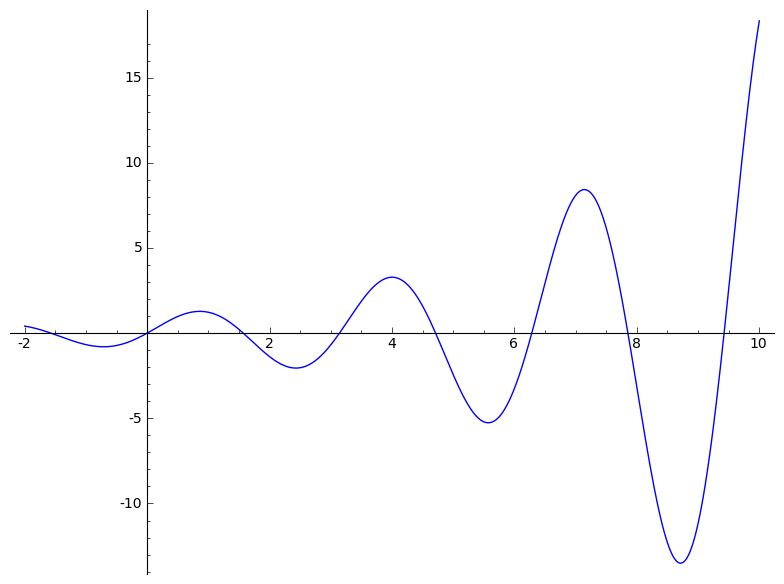
\includegraphics[scale=.1]{imagenes/mu_pos.png}  &
 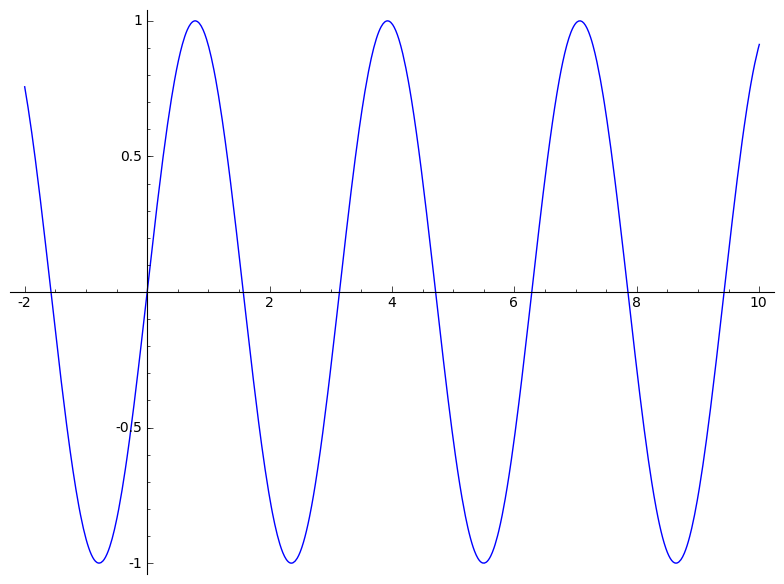
\includegraphics[scale=.1]{imagenes/mu_cero.png}\\
 $\mu<0$ & $\mu>0$ & $\mu=0$\\
\end{tabular}




\end{frame}


\begin{frame}[fragile]{Ecuaciones homogéneas con coeficientes constantes}


3)\textbf{$\boxed{\Delta=p^2-4c=0}$, raices iguales }. Conocemos una solución $\boxed{y_1=e^{-\frac{p}{2}x}}$. Podemos hallar otra
por el método de reducción de orden. Esto consiste en proponer otra solución de la forma $y_2(x)=y_1(x)v(x)$ Dejemos que SAGE nos realice los
cálculos (ver \texttt{uni4b.sage} ).
\begin{sageblock}
x,p=var('x,p')
y=function('y',x)
v=function('v',x)
y1=exp(-p/2*x)
y=v*y1
ecua=y.diff(x,2)+p*y.diff(x)+p^2/4*y==0
ecuav=(ecua/exp(-p/2*x)).simplify_full()
sol=desolve(ecuav,v,ivar=x)
\end{sageblock}
La solución general para $v$ es $v=\sage{sol}$. Así el método mencionado proporciona la solución extra 
\[\boxed{y_2(x)=xe^{-\frac{p}{2}x}}.\]
\end{frame}


\section{Ecuación no homogénea}

\begin{frame}{Ecuaciones no homogéneas. Método coeficientes indeterminados}
\nl \begin{block}{Ecuación no homogénea}
 \boxedeq{\frac{d^2y}{dx^2}+p(x)\frac{dy}{dx}+q(x)y=r(x),}{ec_2_nohom}
donde $p,q,r \in C(I)$ y $r\neq 0$.
 \end{block}

\subsection{Método coeficientes ideterminados}

\nl \begin{block}{Método coeficientes indeterminados}
 
Consiste en buscar soluciones en la misma clase de funciones a la que pertenece $r(x)$. Funciona de manera metódica sólo para algunos tipos de funciones $r(x)$. 
Concretamente para $r(x)$ combinación lineal de funciones polinómicas, exponenciales $e^{\alpha x}$ o trigonométricas $\cos \alpha x$ y $\sen \alpha x$. 
Lo vamos a ilustrar con ejemplos para cada caso.
 \end{block}
 \end{frame}

 
 
 
 
 \defverbatim[colored]\lstI{ 
\begin{lstlisting}
sage: x,p,q,a,A=var('x,p,q,a,A')        
sage: y=function('y',x)
sage: y=A*exp(a*x)     
sage: ecua=y.diff(x,2)+p*y.diff(x)+q*y==exp(a*x)
sage: ecua=(ecua/exp(a*x)).simplify_full()      
sage: ecua
(a^2 + a*p + q)*A == 1
sage: solve(ecua,A)                             
[A == (1/(a^2 + a*p + q))]
\end{lstlisting}
 }
 
 \begin{frame}{Método coeficientes indeterminados. Caso $r(x)=e^{a x}$ y $a^2+pa+q\neq 0$.}
 En esta situación se propone como solución una función de la forma $\boxed{y(x)=Ae^{ax}}$. Usamos SAGE para el cálculos
 
 \lstI
 
 Si $a^2+pa+q\neq 0$,  encontramos la solución particular  $\boxed{y(x)=\frac{1}{(a^2+pa+q)}e^{ax}}$.
 
 
\end{frame}

 
\defverbatim[colored]\lstI{ 
\begin{lstlisting}
sage: x,p,q,a,A=var('x,p,q,a,A')          
sage: y=A*x*exp(a*x)
sage: ecua=y.diff(x,2)+p*y.diff(x)+q*y==exp(a*x)
sage: ecua=(ecua/exp(a*x)).simplify_full()      
sage: ecua
((a^2 + a*p + q)*x + 2*a + p)*A == 1
sage: ecua.subs_expr(a^2 + a*p + q==0)          
(2*a + p)*A == 1

\end{lstlisting}
 }
 \begin{frame}{Método coeficientes indeterminados. Caso $r(x)=e^{a x}$  y $a^2+pa+q= 0$}

En esta situación diremos que la ecuación está en \emph{resonancia}. Más generalmente, diremos que se presenta resonancia cuando $r(x)$ es solución 
del problema homogéneo. 

Propongamos como solución $y(x)=Axe^{ax}$. Hagamos los cálculos con SAGE.

\lstI

Luego, si $2a+p\neq 0$, $\boxed{y(x)=\frac{1}{2a+p}xe^{ax}}$  resuelve el problema.
\end{frame}

\defverbatim[colored]\lstI{ 
\begin{lstlisting}
sage: x,p,q,a,A=var('x,p,q,a,A')               
sage: y=function('y',x)
sage: y=A*x**2*exp(a*x)
sage: ecua=y.diff(x,2)+p*y.diff(x)+q*y==exp(a*x) 
sage: ecua=(ecua/exp(a*x)).simplify_full()      
sage: ecua
((a^2 + a*p + q)*x^2 + 2*(2*a + p)*x + 2)*A == 1
sage: ecua.subs_expr(2*a+p==0,a^2 + a*p + q==0)
2*A == 1

\end{lstlisting}
 }
 
 \begin{frame}{Método coeficientes indeterminados. Caso $r(x)=e^{a x}$, $a^2+pa+q= 0$ y $2a+p=0$}

 Si $2a+p=0$, como también $a^2+pa+q=0$, tenemos que $a$ es una raíz doble de la ecuación $\lambda^2+p\lambda+q=0$. 
 En este caso, proponemos como solución $y(x)=Ax^2e^{ax}$. 
 
 \lstI
 
 Hay que tomar $\boxed{y(x)=\frac{1}{2}x^2e^{ax}}$
 
 
\end{frame}
 
 \defverbatim[colored]\lstI{ 
\begin{lstlisting}
sage: x,p,q,b,A,B=var('x,p,q,b,A,B')             
sage: y=function('y',x)      
sage: y=A*cos(b*x)+B*sin(b*x)
sage: ecua=y.diff(x,2)+p*y.diff(x)+q*y==sin(b*x)
sage: ecua.simplify_full()                      
(b*p*cos(b*x) - (b^2 - q)*sin(b*x))*B - (b*p*sin(b*x) 
...  + (b^2 - q)*cos(b*x))*A == sin(b*x)
sage: ecua=ecua-sin(b*x)                        
sage: ecua
-A*b^2*cos(b*x) - B*b^2*sin(b*x) + (A*cos(b*x) + B*sin(b*x))*q 
...  - (A*b*sin(b*x) - B*b*cos(b*x))*p - sin(b*x) == 0
\end{lstlisting}
 }
 
 
 \begin{frame}{Método coeficientes indeterminados. Caso $r(x)=\sen bx$}
 Proponemos 
 \[y(x)=A\cos x+ B\sen x,\]
 como candidato a solución. 
 
 \lstI
 
 
 
\end{frame}
 
  \defverbatim[colored]\lstI{ 
\begin{lstlisting}
sage: ecua.lhs().coefficient(sin(b*x)).simplify_full()==0
-A*b*p - (b^2 - q)*B - 1 == 0
sage: ecua.lhs().coefficient(cos(b*x)).simplify_full()==0
B*b*p - (b^2 - q)*A == 0
\end{lstlisting}
 }
 
 
 \begin{frame}{Método coeficientes indeterminados. Caso $r(x)=\sen bx$}
La expresión en el miembro de la izquierda es una combinación lineal de las funciones $\cos bx$ y $\sen bx$. Como estas funciones son linealmente independientes
debemos tener que los coeficientes en la combinación lineal deben ser cero
\lstI
Obtenemos un sistema de ecuaciones
\begin{equation}\label{sist_lin_1}
  \left\{\begin{array}{l l}
          -Abp - (b^2 - q)B & = 1\\
          Bbp - (b^2 - q)A &=0
         \end{array}
  \right.
\end{equation}
 
\end{frame}

 \begin{frame}{Método coeficientes indeterminados. Caso $r(x)=\sen bx$}
Para que el sistema tenga solución la matriz de coeficientes debe ser no singular
\[
  0\neq\det \begin{pmatrix}
              -bp & -(b^2-q)\\
              -(b^2-q) & bp
            \end{pmatrix} = -(b^2p^2+(b^2-q)^2)
\]

Podemos suponer $b\neq 0$, de lo contrario la ecuación hubiese sido homogénea. entonces la condición de arriba ocurre si y sólo si 
$p\neq 0$ o $b^2\neq q$. En esa situación encontraremos una solución de la forma
\[
 \boxed{y(x)=A\cos bx + B\sen bx},
\]
donde $A$ y $B$ resuelven \eqref{sist_lin_1}.
\end{frame}



  \begin{frame}{Método coeficientes indeterminados. Caso $r(x)=\sen bx$ con resonancia}\label{eq:forz_res}
Cuando $p=0$ y $b^2= q$ el sistema \eqref{sist_lin_1} puede no tener solución. Notar que en este caso la ecuación queda
\[
 y''+b^2y=\sen bx
\]
Es una ecuación de un oscilador armónico no homogénea. Habíamos visto que justamente $r(x)=\sen bx$ es una solución del problema homogéno. Nuevamente
estamos en una situación de resonancia.  Como en casos anteriores hay que proponer como solución

 \[y(x)=x\left(A\cos x+ B\sen x\right),\]
\end{frame}

 \defverbatim[colored]\lstI{ 
\begin{lstlisting}
sage: x,b,A,B=var('x,b,A,B')        
sage: y=function('y',x)      
sage: y=x*(A*cos(b*x)+B*sin(b*x))
sage: ecua=y.diff(x,2)+b^2*y==sin(b*x)  
sage: ecua=ecua-sin(b*x)    
sage: eql1=ecua.lhs().coefficient(sin(b*x))==0
sage: eql2=ecua.lhs().coefficient(cos(b*x))==0
sage: solve([eql1,eql2],[A,B])
[[A == -1/2/b, B == 0]]
\end{lstlisting}
 }

   \begin{frame}{Método coeficientes indeterminados. Caso $r(x)=\sen bx$ con resonancia}
 \lstI
 
 Encontramos la solución general
 
  \[\boxed{y(x)=-\frac{x}{2b}\cos x}.\]
 
El caso donde $r(x)=\cos bx$ se trata de manera completamente similar.

\end{frame}





 \defverbatim[colored]\lstI{ 
\begin{lstlisting}
sage: PoliQX=QQ['X']
sage: print(PoliQX) 
Univariate Polynomial Ring in X over Rational Field
sage: PoliRX=RR['X'] 
sage: print(PoliRX) 
Univariate Polynomial Ring in X over Real Field with 53 bits of 
...precision
sage: PoliZ3X=Integers(3)['X']
sage: print(PoliZ3X)
Univariate Polynomial Ring in X over Ring of integers modulo 3
sage: p=PoliZ3X([1,1,1])
sage: p
X^2 + X + 1
sage: p+p
2*X^2 + 2*X + 2
sage: p+p+p
0
sage: PoliZ3Xb = PolynomialRing(Integers(3),"X")
sage: PoliZ3X is PoliZ3Xb  
True
sage: X+X    
NameError: name 'X' is not defined
sage: PoliZ3Xc.<X> = Integers(3)["X"]
sage: PoliZ3Xc([1,2,1])+X
X^2 + 1


\end{lstlisting}
 }

   \begin{frame}{Disgresión: \href{http://www.sagemath.org/doc/tutorial/tour_polynomial.html}{anillos de polinomios en SAGE}. Definiendo un anillo de polinomios sobre $\mathbb{Q}$}

\lstI


\end{frame}


 \defverbatim[colored]\lstI{ 
\begin{lstlisting}
sage: P.<X,Y>=QQ["X,Y"]                    
sage: 1+X+X^2+Y^3 in P 
True
sage: p=sum([j*X^j*Y^(3-j) for j in range(4)] )
sage: p in P
True
sage: p
3*X^3 + 2*X^2*Y + X*Y^2
sage: P=QQ[['a'+str(j) for j in range(8)]]
sage: P
Multivariate Power Series Ring in a0, a1, a2, a3, a4,
...a5, a6, a7 over Rational Field
sage: a0 in P
NameError: name 'a0' is not defined
sage: a=P.gens()                          
sage: a
(a0, a1, a2, a3, a4, a5, a6, a7)
sage: a[0] in P
True
sage: type(a[0])
<class 'sage.rings.multi_power_series_ring_element.
...MPowerSeriesRing_generic_with_category.element_class'>
sage: sum([a[j]*j for j in range(8)])
a1 + 2*a2 + 3*a3 + 4*a4 + 5*a5 + 6*a6 + 7*a7
sage: sum([a[j]*j for j in range(8)]) in P
True



\end{lstlisting}
 }

   \begin{frame}{Anillo de polinomios en varias variables}

\lstI


\end{frame}




 \defverbatim[colored]\lstI{ 
\begin{lstlisting}
sage: A=QQ[['a'+str(j) for j in range(5)]]
sage: A
Multivariate Power Series Ring in a0, a1, a2, a3, a4 
....over Rational Field
sage: P.<X>=A["X"]
sage: a=A.gens()
sage: a
(a0, a1, a2, a3, a4)
sage: a[0]*X+a[1]*X^2 in P
True
sage: a[0]*X+a[1]*X^2     
a1*X^2 + a0*X
sage: (a[0]*X+a[1]*X^2)^2 
a1^2*X^4 + 2*a0*a1*X^3 + a0^2*X^2
sage: p=sum([a[j]*X^j for j in range(5)])
sage: p
a4*X^4 + a3*X^3 + a2*X^2 + a1*X + a0




\end{lstlisting}
 }

   \begin{frame}{Anillo de polinomios sobre anillo de polinomios}

\lstI


\end{frame}



 \defverbatim[colored]\lstI{ 
\begin{lstlisting}
sage: grado=4
sage: lista_var=['a'+str(j) for j in range(grado)] 
sage: lista_var+=['b'+str(j) for j in range(grado)]
sage: lista_var+=['p', 'q']                        
sage: A = PolynomialRing(QQ,lista_var)
sage: P=A['X']
sage: r=P([A.gen(i) for i in range(grado)])
sage: r
a3*X^3 + a2*X^2 + a1*X + a0
sage: y=P([A.gen(i) for i in range(grado,2*grado)])
sage: y
b3*X^3 + b2*X^2 + b1*X + b0
sage: eq=y.derivative(2)+y.derivative()*A.gen(2*grado)+y*A.gen(2*grado+1)-r
sage: ecuaciones=[SR(l)==0 for l in eq.coefficients()]
sage: parametros=[SR(A.gen(j)) for j in range(2*grado+2)] 
sage: Sol=solve(ecuaciones,parametros[grado:2*grado])
sage: show(Sol[0])
\end{lstlisting}
 }

\begin{frame}{Método coeficientes indeterminados. Caso $r(x)$ polinomio}
 
Hay que proponer como solución un polinomio, en primera instancia, del mismo grado. Invocando SAGE.

\lstI

\end{frame}

\begin{frame}{Método coeficientes indeterminados. Caso $r(x)$ polinomio}
Encontramos las soluciones

\[
  \begin{split}
      b_{0} &= \frac{a_{0} q^{3} - 6 \, a_{3} p^{3} - {\left(a_{1} p + 2 \, a_{2}\right)} q^{2} + 2 \, {\left(a_{2} p^{2} + 6 \, a_{3} p\right)} q}{q^{4}},\\
      b_{1} &= \frac{a_{1} q^{2} + 6 \, a_{3} p^{2} - 2 \, {\left(a_{2} p + 3 \, a_{3}\right)} q}{q^{3}},\\
      b_{2} &= \frac{a_{2} q - 3 \, a_{3} p}{q^{2}},\\
      b_{3} &= \frac{a_{3}}{q}
  \end{split}
\]
que tienen sentido solo cuando $q\neq 0$.
\end{frame}

\begin{frame}{Método coeficientes indeterminados. Caso $r(x)$ polinomio y resonancia}
El caso $q=0$ es una forma de resonancia. Puede ser tratado como las anteriores resonancias, pero notando que la ecuación se reduce a $y''+py'=r$ conviene 
tomar $v=y'$ como
nueva variable dependiente y reducir la ecuación a una de primer orden.

Por último señalemos que si deseamos resolver un problema de la forma
\[L[y]\equiv y''+py'+qy=r_1(x)+\cdots +r_n(x),\]
donde las funciones $r_i$ son de alguna de las formas descriptas en los casos previos,
entonces la linealidad de $L$ implica que, si $y_i$ 
resuelve $L[y_i]=r_i$, $y=y_1+\cdots +y_n$ resuelve la ecuación deseada. 

\end{frame}

\subsection{Método de variación de los parámetros}

\begin{frame}{Método variación de los parámetros}
Queremos resolver la ecuación
\begin{equation}\label{eq:2orden_gen}
  y''(x)+p(x)y'(x)+q(x)y(x)=r(x).
\end{equation}
Supongamos que contamos con un par de soluciones $y_1$, $y_2$ linealmente independientes de la ecuación homogénea asociada 
\begin{equation}\label{eq:hom_asoc}
  y''(x)+p(x)y'(x)+q(x)y(x)=0.
\end{equation}

El método de \href{http://en.wikipedia.org/wiki/Variation_of_parameters}{variacion de los parámetros} consiste en proponer una solución de la forma
\boxedeq{y(x)=c_1(x)y_1(x)+c_2(x)y_2(x).}{eq:var_param0}

\end{frame}



\begin{frame}{Método variación de los parámetros}

Hay dos funciones incognitas $c_1$ y $c_2$, pero sólo una ecuación. Tendremos por esto libertad de introducir otra condición que consideremos conveniente.

Tenemos
\[
  y'=c_1'y_1+c_1y_1'+c_2'y_2+c_2y_2'.
\]
Pidamos que
\begin{equation}\label{eq:var_param1}
 c_1'y_1+c_2'y_2=0.
\end{equation}
Supuesta esta igualad
\[ y'= c_1y_1'+c_2y_2'.\]
Derivando
\[ y''= c_1'y_1'+c_2'y_2'+c_1y_1''+c_2y_2''.\]


\end{frame}
\begin{frame}{Método variación de los parámetros}

Entonces
\[
 \begin{split}
    r(x)&=y''+py'+qy\\
    &=c_1'y_1'+c_2'y_2'+c_1y_1''+c_2y_2''+p(c_1y_1'+c_2y_2')+q(c_1y_1+c_2y_2)\\
    &=c_1(y_1''+py_1'+qy_1)+c_2(y_2''+py_2'+qy_2)+c_1'y_1'+c_2y_2'\\
    &=c_1'y_1'+c_2'y_2'
 \end{split}
\]
Esta ecuación junto a \eqref{eq:var_param1} nos dan el sistema
\boxedeq{
  \left\{\begin{array}{c c}
            c_1'y_1+c_2'y_2&=0\\
            c_1'y_1'+c_2'y_2'&=r
         \end{array}
  \right. 
}{eq:var_param_sis}
Las incognitas son $c_1'$ y $c_2'$. El determinante de la matriz de coeficientes es precisamente el Wronskiano $W$ de las soluciones $y_1$ e $y_2$, por la suposición
de independencia $W\neq 0$ y por lo tanto el sistema tiene solución única.


\end{frame}

\begin{frame}{Método variación de los parámetros}
Se tiene
\[c_1'=-\frac{\det\begin{pmatrix}
                0 & y_2\\
                r & y_2'
               \end{pmatrix}
}{W}=-\frac{ry_2}{W}
\]
y
\[c_2'=-\frac{\det\begin{pmatrix}
                y_1 & 0\\
                y_1' & r
               \end{pmatrix}
}{W}=\frac{ry_1}{W}
\]
\end{frame}

\begin{frame}{Método variación de los parámetros}
En consecuencia
\boxedeq{c_1=-\int\frac{ry_2}{W}dx}{eq:c1}
y
\boxedeq{c_2=\int\frac{ry_1}{W}}{eq:c2}

Usando estas fórmulas y \eqref{eq:var_param0} obtenemos una solución particular del sistema. La solución general es la suma de la particular más
una solución general del homogéneo. Esta última solución general se escribe como una combinación lineal genérica entre $y_1$ e $y_2$.
\end{frame}
 \defverbatim[colored]\lstI{ 
\begin{lstlisting}
sage: x=var('x')
sage: y1=sin(x)
sage: y2=cos(x)
sage: W=y1*y2.diff()-y1.diff()*y2
sage: W.simplify_full() #chequeamos independencia
-1
sage: r=csc(x)
sage: y=(r*y1/W).integral(x)*y2-(r*y2/W).integral(x)*y1 #formula
sage: y
-x*cos(x) + log(sin(x))*sin(x)
sage: c1,c2=var('c1,c2')
sage: z=y+c1*y1+c2*y2 #solucion general
sage: (z.diff(x,2)+z-r).simplify_trig()
0
sage: #resolvemos pvi
sage: C=solve([z(x=pi/2)==0,z.diff(x).subs(x=pi/2)==1],[c1,c2])
sage: C
[[c1 == 0, c2 == 1/2*pi - 1]]
sage: A,B=C[0]
sage: y=z.subs_expr(A,B)
sage: y
1/2*(pi - 2)*cos(x) - x*cos(x) + log(sin(x))*sin(x)
sage: y(x=pi/2)
0
sage: y.diff()(x=pi/2)
1

\end{lstlisting}
 }

\begin{frame}{Método variación de los parámetros}
\textbf{Ejemlo} Resolver el siguiente pvi $y''+y=\csc x$, $y\left(\tfrac{\pi}{2}\right)=0$ y  $y'\left(\tfrac{\pi}{2}\right)=1$.
\lstI
\end{frame}

\section{Conclusiones}

\begin{frame}{Conclusiones}
\begin{enumerate}
 \item Si podemos encontrar dos soluciones linealmente independientes de una ecuación lineal homogénea de segundo orden, tenemos la solución general a traves de 
 combinaciones lineales.
 \item Si tenemos una solución no trivial de una ecuación lineal homogénea de segundo orden podemos hallar otra por el método de reducción de orden.
 \item Podemos resolver completamente una ecuación lineal homogénea de segundo orden con coeficientes constantes.
 \item Podemos resolver algunos problemas no homogéneos por el método de coeficientes indeterminados.
 \item Si conocemos las soluciones del problema homogéneo podemos resolver, en teoría, el no homogéneno para cualquier $r(x)$ por el método de variación 
 de los parámetros
\end{enumerate}

\end{frame}

\section{Aplicaciones}

\begin{frame}{Aplicaciones. Vibraciones mecánicas }
 
\textbf{Problema:} Estudiar el movimiento de un resorte (cómo el de la unidad anterior) pero suponer que además de actuar sobre la masa la fuerza elástica del resorte,
tenemos una fuerza de fricción debida ala resistencia del medio. Por la acción de esta fuerza, se dice que es un sistema resorte-masa amortiguado.
Además suponemos que hay otra fuerza $F$ externa y que sólo depende de $t$. Por ejemplo si el resorte se colocase verticalmente y se dejase suspendida 
la masa, $F$ sería la fuerza de gravedad. Si la masa estuviese hecha de metal, $F$ podría ser una fuerza provista por un imán. Por la acción de esta fuerza el sistema se 
dice forzado. Por consiguiente el sistema completo, con la acción de las tres fuerzas, se denomina un sistema resorte-masa, amortiguado y forzado.
\end{frame}

\begin{frame}{Aplicaciones. Vibraciones mecánicas }

La fuerza elástica del resorte se modeliza con la Ley de Hooke. 
Para la amortiguación, supongamos que su módulo  es proporcional a la velocidad de la masa. La constante de proporcionalidad $c$ se llama coeficiente de 
\href{http://es.wikipedia.org/wiki/Viscosidad}{viscosidad}. La dirección y sentido de la fuerza amortiguadora es siempre contraria 
al movimiento. Por el principio de conservación de la energía, vemos que la fuerza de amortiguación siempre realiza un trabajo $W$ negativo, por consiguiente
hace perder energía cinética. De la fuerza externa $F$ no sabemos nada en principio. Por todo lo expuesto, si ponemos un sistema 
de coordenadas con origen en la posición de equilibrio del sistema masa-resorte y si $x(t)$ es la posición de la masa en el momento $t$, la ecuación que gobierna 
el sistema masa-resorte con amortiguación y forzamiento es 

\boxedeq{mx''(t)\underbrace{=}_\text{2° Ley Newton}\underbrace{-kx(t)}_
\text{Hooke}\underbrace{-cx'(t)}_\text{Amortiguación}+\underbrace{F(t)}_\text{Fuerza externa}}{eq:res_amor_for}

\end{frame}

\begin{frame}{ Vibraciones amortiguadas no forzadas ($c>0$, $F=0$) }
 
Escribamos la ecuación \eqref{eq:res_amor_for} de la siguiente froma

\begin{equation}\label{eq:res_amor}
  \boxed{x''(t)+2\mu x'(t)+\omega^2x=0}\quad \mu:=\frac{c}{2m},\omega:=\sqrt{\frac{k}{m}}. 
\end{equation}

Las raíces de la ecuación característica son
\[
 \boxed{\lambda_{1,2}=-\mu\pm\sqrt{\Delta},\quad \Delta:=\mu^2-\omega^2}
\]

\textbf{Caso $\Delta>0$.} Aquí la viscocidad es ``grande'' relativa ala rigidez $k$. Se dice que el sistema está sobreamortiguado. En este caso tenemos dos soluciones
linealmente independientes y la solución general es de la forma
\[x(t)=c_1e^{\lambda_1t}+c_2e^{\lambda_2t}\]
Notar que $\lambda_1,\lambda_2<0$.
\end{frame}



\defverbatim[colored]\lstI{ 
\begin{lstlisting}
sage: lambda1,lambda2=var('lambda1,lambda2')
sage: t=var('t')
sage: x=c1*e^(lambda1*t)+c2*e^(lambda2*t)
sage: x0=var('x0')
sage: C=solve([x(t=0)==x0,x.diff(t).subs(t=0)==0],
....[c1,c2],solution_dict=True)
sage: C
[{c2: lambda1*x0/(lambda1 - lambda2), c1: -lambda2*x0/(lambda1 - lambda2)}]
sage: x=x.subs(C[0])
sage: x.show()
sage: latex(x)
-\frac{\lambda_{2} x_{0} e^{\left(\lambda_{1} t\right)}}{\lambda_{1} - \lambda_{2}} + 
...\frac{\lambda_{1} x_{0} e^{\left(\lambda_{2} t\right)}}{\lambda_{1} - \lambda_{2}}



\end{lstlisting}
 }
\begin{frame}{ Vibraciones amortiguadas no forzadas ($c>0$, $F=0$) }
Supongamos que el sistema masa-resorte parte del resposo $x'(0)=0$ y de una posición indeterminada $x_0$. Resolvamos este pvi
\lstI

\boxedeq{
  x(t)= x_0\left\{ \frac{\lambda_{1}  
  e^{\lambda_{2} t}}{\lambda_{1} - \lambda_{2}}-\frac{\lambda_{2} e^{\lambda_{1} t}}{\lambda_{1} - \lambda_{2}}\right\}
}{eq:sol_sub_amor}
\end{frame}



\defverbatim[colored]\lstI{ 
\begin{lstlisting}
sage: x=x.subs({lambda1:-1,lambda2:-2,x0:1})
sage: x.plot((x,0,10))

\end{lstlisting}
 }

\begin{frame}{ Vibraciones amortiguadas no forzadas ($c>0$, $F=0$) }
La masa podría haber pasado por la posición de equilibrio sólo en el pasado puesto que $x(t)=0$ cuando
\[\boxed{t=\frac{1}{\lambda_1-\lambda_2}\ln\frac{\lambda_1}{\lambda_2}<0}\]
 
 \lstI 
 
 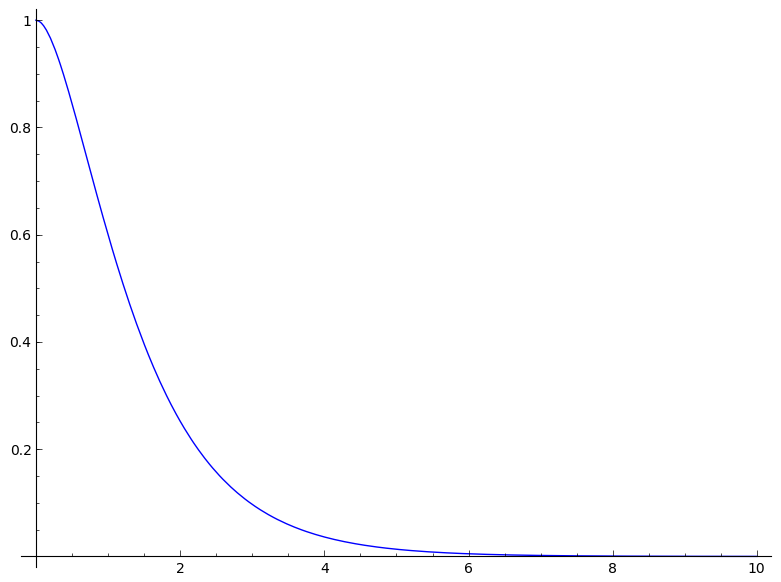
\includegraphics[scale=.2]{imagenes/sobreamortiguado.png}


\end{frame}


\begin{frame}{ Vibraciones amortiguadas no forzadas ($c>0$, $F=0$) }

\begin{center}

\begin{figure}[h]
\animategraphics[controls, scale=.4]{15}{res_sobre/res_sobre-}{0}{60}
\vspace{.5cm}
\caption{Masa-resorte sobreamortiguado}
\end{figure}
\end{center}
\end{frame}



\defverbatim[colored]\lstI{ 
\begin{lstlisting}
sage: c1,c2=var('c1,c2')
sage: mu=var('mu')
sage: t=var('t')
sage: x=e^(-mu*t)*(c1+c2*t)
sage: x0=var('x0')
sage: C=solve([x(t=0)==x0,x.diff(t).subs(t=0)==0],[c1,c2],solution_dict=True)
sage: C
[{c2: mu*x0, c1: x0}]
sage: x=x.subs(C[0]).subs({mu:.1,x0:1})
sage: x.plot((x,0,100))

\end{lstlisting}
 }



\begin{frame}{ Vibraciones amortiguadas no forzadas ($c>0$, $F=0$) }
\textbf{Caso $\Delta=0$.} En esta situación se dice que hay amortiguación crítica. Las raíces son iguales $\lambda_1=\lambda_2=-\mu$. Sabemos que
\boxedeq{x_1(t)=c_1e^{-\mu t}+c_2te^{-\mu t}=e^{-\mu t}\{c_1+c_2t\}}{eq:sol_gen_crit}
 \lstI 
 \begin{center}
   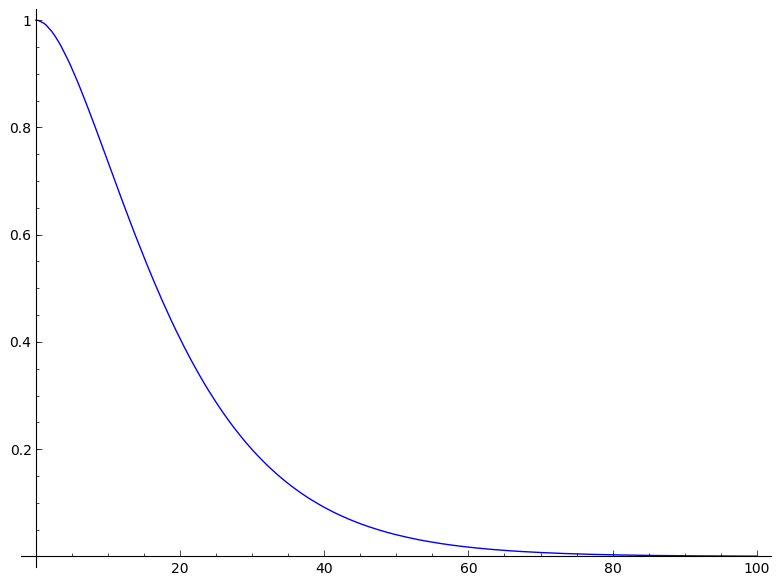
\includegraphics[scale=.1]{imagenes/crit_amortiguado.png}
 \end{center}


 


\end{frame}

\defverbatim[colored]\lstI{ 
\begin{lstlisting}
sage: c1,c2=var('c1,c2')
sage: mu=var('mu')
sage: nu=var('nu')
sage: x0=var('x0')
sage: x=e^(-mu*t)*(c1*cos(nu*t)+c2*sin(nu*t))
sage: t=var('t')
sage: C=solve([x(t=0)==x0,x.diff(t).subs(t=0)==0],[c1,c2],solution_dict=True)
sage: x=x.subs(C[0]).subs({mu:.1,nu:4,x0:1})
sage: x.plot((x,0,100))


\end{lstlisting}
 }
\begin{frame}{ Vibraciones amortiguadas no forzadas ($c>0$, $F=0$) }
\textbf{Caso $\Delta<0$.} Caso subamortiguado, $\lambda_{1,2}=-\mu\pm\nu i$ con $\nu=\sqrt{|\Delta|}=\sqrt{|\omega^2-\mu^2|}$.
La solución general viene dada por

\boxedeq{x(t)=e^{-\mu t}\left\{ c_1\cos \nu t+c_2\sen \nu t    \right\}}{eq:sol_gen_sub}
 \lstI 
 \begin{center}
   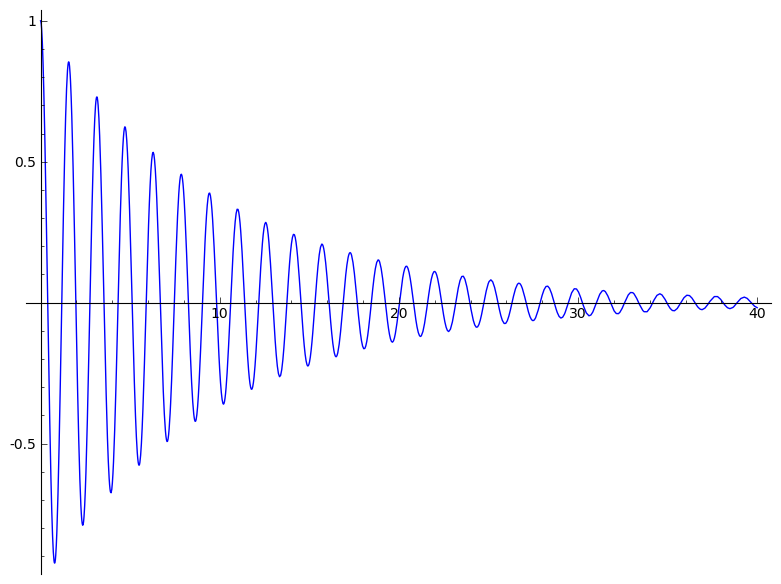
\includegraphics[scale=.1]{imagenes/subamortiguado.png}
 \end{center}
 


\end{frame}
 


\begin{frame}{ Vibraciones amortiguadas no forzadas ($c>0$, $F=0$) }
\begin{figure}[h]
\animategraphics[controls, scale=.4]{15}{res_sub/res_sub-}{0}{60}
%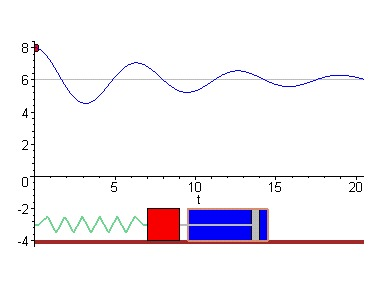
\includegraphics[scale=.4]{res_sub/res_sub-0.jpg}
\vspace{.5cm}
\caption{Masa-resorte subamortiguado}
\end{figure}
 
\end{frame}


\begin{frame}{ Vibraciones amortiguadas no forzadas ($c>0$, $F=0$) }
Se suele escribir la ecuación \eqref{eq:sol_gen_sub} de otra forma. Expresemos el vector $(c_1,c_2)$ en 
coordenadas polares. 
\[
c_1=\rho\cos\alpha,\quad c_2=\rho\sen\alpha.
\]
Entonces
\[
 x(t)=e^{-\mu t}\left\{ c_1\cos \nu t+c_2\sen \nu t    \right\}=\boxed{\rho e^{-\mu t}\cos(\nu t-\alpha)}.
\]
Llamaremos este régimen \emph{movimiento  cuasi-oscilatorio}. Se ejecutan vibraciones que se van amortiguando
de \href{http://es.wikipedia.org/wiki/Frecuencia}{frecuencia}
\[
  f=\frac{1}{\text{período}}=\frac{\nu}{2\pi},\quad \nu=\sqrt{\omega^2-\mu^2}=\sqrt{\left(\frac{k}{m}\right)^2-
  \left(\frac{c}{2m}\right)^2}.
\]
En lugar de la frecuencia se suele considerar la 
\href{http://luz.izt.uam.mx/mediawiki/index.php/Frecuencia_angular}{frecuencia angular} que se define como 
$2\pi f$. La ventaja de esta definición es que la frecuencia ángular de la función de arriba es
$\nu$. 
\end{frame}



\begin{frame}{ Vibraciones amortiguadas no forzadas ($c>0$, $F=0$) }
\textbf{Ejercicio:} En cualquiera de las situaciones descriptas, $x(t)\to 0$ y $x'(t)\to 0$, cuando $t\to\infty$. 
Es decir, la masa se va deteniendo.                                                                                                                                                                                                                                                                         
 


\end{frame}


\begin{frame}{ Vibraciones no amortiguadas y forzadas ($c=0$, $F\neq 0$) }
Vamos a considerar una fuerza externa oscilatoria de frecuencia angular $\omega_0$ y amplitud $F_0$. Tenemos que resolver
\boxedeq{x''(t)+\omega^2 x(t)=F_0\cos(\omega_0 t).}{eq:ecua_2orden_nohom}
Usaremos el método de coeficientes indeterminados y SAGE. Antes, recordar que si $\omega=\omega_0$ estamos en 
resonancia. Tendremos que considerar ese caso por separado. Supongamos pues $\omega\neq\omega_0$.

El siguiente código se puede encontrar en la carpeta \texttt{scripts} del repositorio 
\href{https://github.com/fdmazzone/Ecuaciones_Diferenciales}{GitHub} de esta  materia. El script se denomina \texttt{osc\_arm\_forz\_noamort.sage} 
 

\end{frame}



\begin{frame}{ Vibraciones no amortiguadas y forzadas ($c=0$, $F\neq 0$) }
 \lstinputlisting{scripts/osc_arm_forz_noamort.sage}

 
Notar que el determinante del sistema de ecuaciones algebraicas es $-(\omega-\omega_0)^2$. Luego la matriz 
es no singular sólo en no resonancia. 

La solución general del problema es la solución particular que acabamos de obtener más una solución 
general del homogéneo que sabemos es una combinación lineal generica entre $\cos \omega t$ y $\sin \omega t$.


 
 
\end{frame}

\begin{frame}{ Vibraciones no amortiguadas y forzadas ($c=0$, $F\neq 0$) }
\boxedeq{x(t)=\frac{F_{0} \cos\left(\omega_{0} t\right)}{\omega^{2} - \omega_{0}^{2}}+
c_1\cos(\omega t)+c_2\sin(\omega t).}{eq:sol_gen_noamort_forz}

Como ya hemos visto, considerando las coordenadas polares $\rho$ y $\alpha$ de $c_1,c_2)$
podemos reescribir la solución 


\[x(t)=\frac{F_{0} \cos\left(\omega_{0} t\right)}{\omega^{2} - \omega_{0}^{2}}+
\rho\cos(\omega t-\alpha)
\]

Vemos que el movimiento es la superposición de dos movimientos oscilatorios de frecuencias $\omega$, que se
denomina la \emph{frecuencia natural} del resorte, y $\omega_0$ que se denomina \emph{frecuencia impresa}.
 
\end{frame}

\defverbatim[colored]\lstI{ 
\begin{lstlisting}
sage: t,omega,omega0,F0,rho,alpha=var('t,omega,omega0,F0,rho,alpha')
sage: x=F0/(omega^2-omega0^2)*cos(omega0*t)+rho*cos(omega*t-alpha)  
sage: assume(-pi<alpha, alpha<2*pi)
sage: solve([x(t=0)==0,x.diff(t).subs(t=0)==0],[rho,alpha])         
[omega*rho*sin(alpha) == 0, rho*cos(alpha) + F0/(omega^2 - omega0^2) == 0]
sage: x0=x(alpha=0)
sage: sol=solve([x0(t=0)==0,x0.diff(t).subs(t=0)==0],rho,\
solution_dict=True) 
sage: x0=x0.subs(sol[0])
sage: x0.factor().show()

\end{lstlisting}
 }


\begin{frame}{ Vibraciones no amortiguadas y forzadas ($c=0$, $F\neq 0$) }
Resolvamos el pvi
\[
 \left\{\begin{array}{l}
         x''(t)+\omega^2x(t)=F_0\cos(\omega_0 t),\\
         x'(0)=x(0)=0\\
        \end{array}
\right.
\]


\lstI

\[x(t)=-\frac{F_{0} \cos\left(\omega t\right)}{\omega^{2} - \omega_{0}^{2}} + \frac{F_{0} \cos\left(\omega_{0} t\right)}{\omega^{2} - \omega_{0}^{2}}
\]
\end{frame}

\defverbatim[colored]\lstI{ 
\begin{lstlisting}
sage: x1=x0.subs({F0:1,omega:1,omega0:.9}) 
sage: x1.plot(x,0,200)
\end{lstlisting}
 }


\begin{frame}{ Vibraciones no amortiguadas y forzadas ($c=0$, $F\neq 0$) }
Ahora usemos la identidad $\cos(a-b)-cos(a+b)=2\sen a\sen b$, con $a=\frac12 (\omega+\omega_0)$ y
$b=\frac12 (\omega-\omega_0)$. Deducimos
\boxedeq{%
  x(t)=\frac{2F_{0} }{\omega^{2} - \omega_{0}^{2}}\sen (\omega-\omega_0)t \sen (\omega+\omega_0)t. 
}{eq:sol_gen_pulsos}
Esta  expresión la podemos ver como una onda de frecuencia  grande $\omega+\omega_0$ modulada por una de frecuencia 
chica $\omega-\omega_0$. 
\lstI
\begin{center}
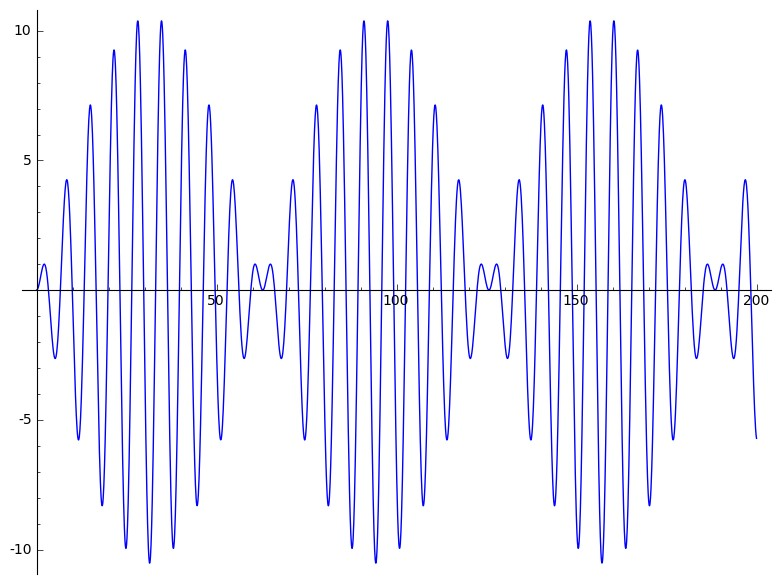
\includegraphics[scale=.15]{imagenes/batido.jpg}
\end{center}


\end{frame}
\defverbatim[colored]\lstI{ 
\begin{lstlisting}
sage: limit(x0,omega0=omega)
1/2*F0*t*sin(omega*t)/omega
\end{lstlisting}
 }

\begin{frame}{ Vibraciones no amortiguadas y forzadas ($c>0$, $F\neq 0$) }
Calculemos el límite $\lim_{\omega_0\to\omega}x(t)$,
\lstI

\[x(t)=\frac{F_{0} t \sin\left(\omega t\right)}{2 \, \omega}
\]
El caso $\omega=\omega_0$ es el caso con resonancia, que debemos resolver como fue indicado en la página \ref{eq:forz_res}, 
esto es proponiendo como solución $y(x)=x\left(A\cos x+ B\sen x\right)$. El siguiente código sage muestra que la solución es la misma función
que la obtenida por el proceso de límite de los casos sin resonancia.

\lstinputlisting{scripts/osc_arm_forz_noamort_res.sage}

\end{frame}

 \begin{frame}{ Vibraciones no amortiguadas y forzadas ($c>0$, $F\neq 0$) } 
Se producen ``vibraciones'' no acotadas.
\begin{center}
 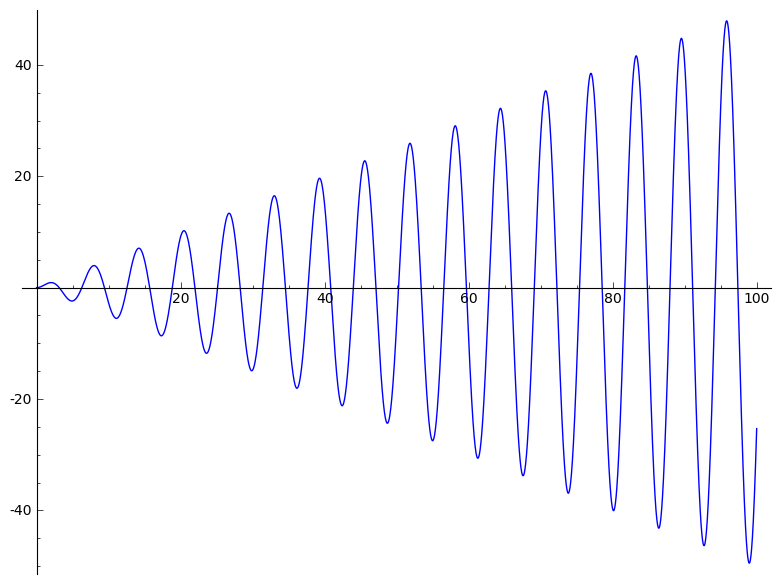
\includegraphics[scale=0.3]{imagenes/osc_arm_forz_res.png}
\end{center}

Ver la notebook \texttt{batido.sws}. En la wiki \href{http://wiki.sagemath.org/interact/misc\#Hearing_a_trigonometric_identity}{Hearing a trigonometric identity}
se puede escuchar ondas sonoras con los fenómenos de resonancia y batido.

\end{frame}



\begin{frame}{ Vibraciones amortiguadas y forzadas ($c>0$, $F\neq 0$) }
Vamos a considerar una fuerza externa oscilatoria de frecuencia $\omega_0$ y amplitud $F_0$. Tenemos que resolver
\boxedeq{x''(t)+2\mu x'(t)+\omega^2 x(t)=F_0\cos(\omega_0 t).}{eq:ecua_2orden_amort_nohom}
\lstinputlisting{scripts/osc_arm_forz_amort.sage}


\end{frame}



\defverbatim[colored]\lstI{ 
\begin{lstlisting}
sage: rho=sqrt(A**2+B**2).subs(SolAB[0]).simplify_full()                                         
sage: show(rho)
\end{lstlisting}
 }


 
\begin{frame}{ Vibraciones amortiguadas y forzadas ($c>0$, $F\neq 0$) } 
\boxedeq{x(t)=
  \frac{2 \, F_{0} \mu \omega_{0} \sin\left(\omega_{0} t\right)}{\omega^{4} + \omega_{0}^{4} + 2 \,
  {\left(2 \, \mu^{2} - \omega^{2}\right)} \omega_{0}^{2}} + \frac{{\left(F_{0} \omega^{2} - 
  F_{0} \omega_{0}^{2}\right)} \cos\left(\omega_{0} t\right)}{\omega^{4} + 
  \omega_{0}^{4} + 2 \, {\left(2 \, \mu^{2} - \omega^{2}\right)} \omega_{0}^{2}}
}{eq:SolGennoHom}


Es un movimiento oscilatorio de frecuencia angular $\omega_0$. Podemos escribir $x(t)=\rho\cos(\omega_0 t-\alpha)$, 
donde $(\rho,\alpha)$ son las coordenadas polares de $(A,B)$. En particular $\rho=\sqrt{A^2+B^2}$
Recurrimos nuevamente a SAGE
\lstI
\[
\rho(\omega_0)=\frac{F_{0}}{\sqrt{\omega^{4} + \omega_{0}^{4} + 2 \, {\left(2 \, \mu^{2} - \omega^{2}\right)} \omega_{0}^{2}}}=
\frac{F_{0}}{\sqrt{(\omega^2-\omega_0^2)^2+4\mu^2\omega_0^2}}
\]
\end{frame}

\defverbatim[colored]\lstI{ 
\begin{lstlisting}
sage: plot(rho.subs({F0:1, mu:.1,omega:5},(omega0,0,10) )
\end{lstlisting}
 }



\begin{frame}{ Vibraciones amortiguadas y forzadas ($c>0$, $F\neq 0$) } 
\[\alpha=\atan2\left(  {{\omega^{2} - 
  \omega_{0}^{2}} }  ,  {2 \,  \mu \omega_{0} }   \right)
\]
En una consola de sage entrar \texttt{atan2?} para averiguar que función es $\atan2$. 

Grafiquemos la función $\rho(\omega_0)$ para $\omega=5$ y $\mu=0.1$. 

\lstI 
\begin{center}
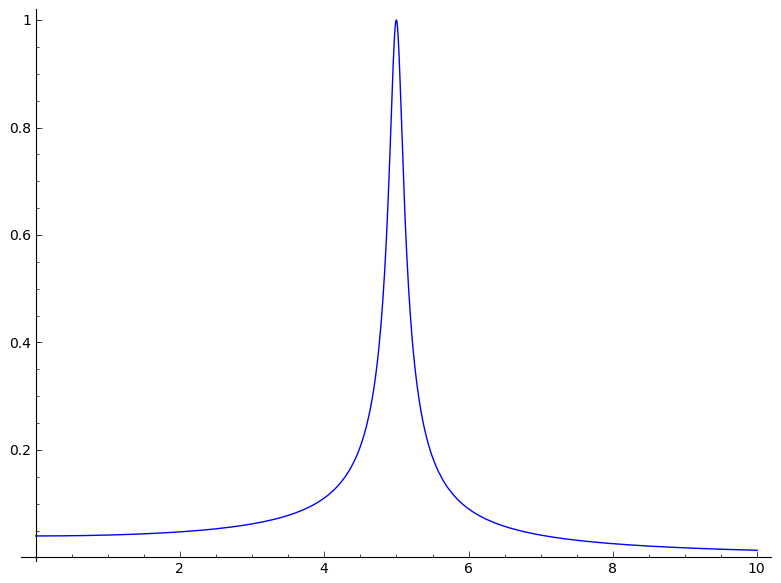
\includegraphics[scale=.2]{imagenes/rho_graf.png}
\end{center}

\end{frame}




 \defverbatim[colored]\lstI{ 
\begin{lstlisting}
sage: sol=solve(rho.diff(omega0),omega0)
sage: sol
[omega0 == -sqrt(-2*mu^2 + omega^2), omega0 == sqrt(-2*mu^2 + omega^2), omega0 == 0]
sage: rho.diff(omega0,2).subs(sol[1]).simplify_full().show()
\end{lstlisting}
 }
 \defverbatim[colored]\lstII{ 
\begin{lstlisting}
sage: sol[1].rhs().subs({mu:.1,omega:5})                         
4.99799959983992
\end{lstlisting}
 } 
 \begin{frame}{ Vibraciones amortiguadas y forzadas ($c>0$, $F\neq 0$) } 
La función tiene un notorio máximo  cerca de $\omega_0=5$. Seguramente es debido a la aparición de resonancias. Hallemos el punto de máximo exacto. 
\lstI
Si $2\mu^2<\omega$ tendremos un máximo (en realidad un máximo local) en  $\omega_{0} = \sqrt{-2 \, \mu^{2} + \omega^{2}}$. En el ejemplo que graficamos
el máximo ocurre en
\lstII
Vale decir, un oscilador armónico en reposo es más sensible a exitaciones en ciertas frecuencias, aproximadamente la frecuencia
natural del resorte cuando el coeficiente de viscocidad $c=2m\mu$ es chico. Esto es utilizado para diseñar dispositivos que captan ondas sísmicas.


\end{frame}

 \begin{frame}{ Vibraciones amortiguadas y forzadas ($c>0$, $F\neq 0$) } 
 Hasta aquí hemos encontrado una solución particular del sistema no homogéneo. Para encontrar una solución general deberíamos adicionar a la particular que disponemos
 una solución general $x_g(t)$  de la ecuación homogénea.  La forma de esta solución general es de alguno de los tipos \ref{eq:sol_gen_sub},
 \ref{eq:sol_gen_crit} o \ref{eq:sol_sub_amor}. Sin embargo no nos importa ahora la fórmula explícita de estas soluciones, sino que nos interesa resaltar que 
 tratese del tipo que se trate, se satisface que $\lim_{t\to\infty}x_g(t)=0$. Por este motivo, vamos a decir que esta parte de la solución es 
 \emph{transitoria}. En cambio la solución que prevalece en el tiempo dada por \eqref{eq:SolGennoHom} la denominaremos solución \emph{estacionaria}.
 
  
\end{frame}
 
 
 \begin{frame}{Un poco de mecánica celeste}
 
 Vamos a considerar ahora el problema del movimiento de un planeta, digamos la Tierra, de masa $m_{\earth}$ alrededor del sol de masa $m_{\sun}$. Como 
 $m_{\sun}\gg m_{\earth}$ vamos a ignorar la fuerza que actúa sobre el Sol debido a la atracción gravitatoria de la Tierra. Esta suposición, aunque falsa, la hacemos 
 por simplicidad. No obstante, con sólo un poco de trabajo, el caso más general se reduce al tratado aquí. Ver el trabajo final de la Lic. Matemática de Leopoldo Buri,
 para una deducción más cuidadosa. Vamos a suponer además que el movimiento del planeta se retringe a un plano. Esta afirmación es cierta y aunque su demostración
 es sencilla no la desarrollaremos aquí. 
 
 Supongamos un sistema de coordenadas cartesianas sobre el plano en que se realiza el movimiento orbital del planeta. Asumimos el Sol en el origen de coordenadas y en 
 reposo. Como no actúa fuerza sobre él, permanecerá en esa situación. Vamos a suponer que la posición de la Tierra es $\v{r}$.

  
 
  
  \end{frame}

  

\begin{frame}{Un poco de mecánica celeste}
   Los dos ingredientes básicos para derivar la leyes de movimiento del planeta son la 
   \href{http://es.wikipedia.org/wiki/Leyes_de_Newton\#Segunda_ley_de_Newton_o_ley_de_fuerza}{Segunda Ley de Newton} y la
   \href{http://es.wikipedia.org/wiki/Ley_de_gravitación_universal}{Ley Gravitación Universal}. Ya  hemos considerado ambas con anterioridad. 
   
  Según  la Ley de Gravitación Universal, la magnitud de la fuerza de gravedad es proporcional a $\frac{m_{\earth}m_{\sun}}{d^2}$, donde $d$ es la distancia tierra-sol. 
  A la constante de proporcionalidad la llamaremos, como es costumbre, $G$. La dirección de la fuerza gravitatoria es la de la recta que une los  dos astros y 
  el sentido es tal que la fuerza atrae los cuerpos. Vale decir, la dirección y sentido de la 
  fuerza de gravedad vienen dados por el versor $-\v{r}/r$, donde $r=|\v{r}|$. Luego se debe satisfacer que
  \[Gm_{\earth}\frac{d^2\v{r}}{dt^2}=-\frac{Gm_{\earth}m_{\sun}}{r^2}\frac{\v{r}}{r}=-Gm_{\earth}m_{\sun}\frac{\v{r}}{r^3}. \]
   
   
\end{frame}

\begin{frame}{Un poco de mecánica celeste}
  
  Es decir
  \boxedeq{\frac{d^2\v{r}}{dt^2}=-\mu\frac{\v{r}}{r^3}\quad\text{donde } \mu:=Gm_{\sun}}{eq:grav}

  Esta ecuación se conoce como la \href{http://es.wikipedia.org/wiki/Problema_de_los_dos_cuerpos}{ecuación de los dos cuerpos}.
  Dado que esta ecuación entraña, a su vez, tres ecuaciones escalares, una por cada
  componente de $\v{r}$, se nos presenta aquí  un \emph{Sistema de Ecuaciones Diferenciales}. No sabemos resolver sistemas de ecuaciones. No obstante vamos
  a ver como podemos reducir la ecuación anterior, mediante ingeniosos cambios de 
  variables, a ecuaciones diferenciales que sabemos resolver.
 
   
\end{frame}
    
\begin{frame}{Un poco de mecánica celeste}
Vamos a usar coordenadas polares $(r,\theta)$ y los versores $\v{u}_r:=(\cos\theta,\sen\theta)$ y $\v{u}_{\theta}:=(-\sen\theta, \cos\theta)$. Notar que 
$\v{u}_r \perp \v{u}_{\theta}$ y por consiguiente $\mathcal{B}:=\{\v{u}_r , \v{u}_{\theta}\}$ forma  una base del espacio euclideano 2-dimensional. Usaremos este hecho 
para representar distintos vectores como combinación lineal de vectores de la base.  Los cálculos, como es ya habitual, se los dejaremos a SAGE, pero esta vez
usaremos \href{ http://www.sagemath.org/doc/tutorial/sagetex.html}{\textsf{Sage\TeX}} como interfaz de SAGE. 
\textsf{Sage\TeX} permite incrustar código y outputs  de SAGE dentro de un archivo \LaTeX .

Todos los cálculos que realizamos los pueden encontrar en el script \texttt{2cuerpos.sage} dentro de la carpeta scripts en 
el repositorio de \href{https://github.com/fdmazzone/Ecuaciones_Diferenciales}{GitHub} 
que mantiene materiales de este curso. Ver el siguiente enlace

\href{https://github.com/fdmazzone/Ecuaciones_Diferenciales}{https//github.com/fdmazzone/Ecuaciones\_Diferenciales}

   
\end{frame} 
  
\begin{frame}[fragile]{Un poco de mecánica celeste}
Primero declaramos las variables y asignamos los vectores $\v{u}_r$, $\v{u}_{\theta}$ y el vector 
$\v{r}$ al que llamamos \texttt{pos}. 
\begin{sageblock}
t,mu=var('t,mu')
x=function('x',t)
y=function('y',t)
r=function('r',t)
theta=function('theta',t)
u_r=vector([cos(theta),sin(theta)])
u_theta=vector([-sin(theta),cos(theta)])
pos=(r*u_r).column()
\end{sageblock}


Como vamos a necesitar representar vectores en la base $\mathcal{B}=\{\v{u}_r , \v{u}_{\theta}\}$, construímos una matriz
con los vectores de la base en las columnas.
\begin{sageblock}
 M=matrix([[cos(theta),-sin(theta)],\
 [sin(theta),cos(theta)]])
\end{sageblock}

\end{frame} 

\begin{frame}[fragile]{Un poco de mecánica celeste}
Demosle un vistazo a $M$
\[M:=\sage{M}.\]
Concretamente queremos representar el vector aceleración $\v{a}:=\tfrac{d^2\v{r}}{dt^2}$ en la base $\mathcal{B}$, para ello  debemos resolver $MX=\v{a}$, donde $X$ y 
$\v{a}$ los asumimos vectores columna. Con SAGE lo hacemos en un periquete
\begin{sageblock}
  sol=M.solve_right(pos.derivative(t,2))
  a1=sol[0].simplify_full()
  a2=sol[1].simplify_full()
\end{sageblock}
Obtenemos asi las dos componetes de $\v{a}$.
\end{frame}


\begin{frame}[fragile]{Un poco de mecánica celeste}
En la notación de SAGE
\[
 \v{a}=\left(\begin{array}{c}
              \sage{a1}\\
              \sage{a2}
             \end{array}
 \right)
\]
En la que nos gusta más

\[
 \v{a}=\left(\begin{array}{c}
              \ddot{r}-r\dot{\theta}^2 \\
              r\ddot{\theta}+2\dot{r}\dot{\theta}
             \end{array}
 \right)=
 \left(\begin{array}{c}
              \ddot{r}-r\dot{\theta}^2 \\
              \frac{1}{r}\frac{d}{dt} \left( r^2\dot{\theta} \right) 
             \end{array}
 \right)
\]
\end{frame}

\begin{frame}{Un poco de mecánica celeste}
  El vector aceleración debe ser igual a la fuerza por unidad de masa $-\mu \v{r}/r^3$. Notemos que esta fuerza es 
  \href{http://es.wikipedia.org/wiki/Campo_central}{central}, es decir tiene componente nula
  respecto al vector $\v{u}_{\theta}$. Por consiguiente se debe satisfacer que
    \[\frac{1}{r}\frac{d}{dt} \left( r^2\dot{\theta} \right)=0\Longleftrightarrow  \exists h\in\mathbb{R}: \boxed{ r^2\dot{\theta}=h}. \]
\begin{tabular}{m{5cm} m{5cm}}


  Hemos derivado la \href{http://es.wikipedia.org/wiki/Leyes_de_Kepler}{Segunda Ley de Kepler}: El radio vector barre áreas iguales en tiempos iguales.
  &
  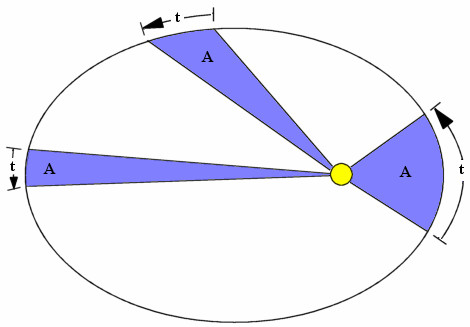
\includegraphics[scale=.3]{imagenes/2leykepler.jpeg}\\
\end{tabular}
\end{frame}
  
  
  
\begin{frame}[fragile]{Un poco de mecánica celeste}
En la dirección radial $\v{u}_r$ la componente de la fuerza es $-\mu/r^2$. Es decir se satisface la ecuación
\[
  \ddot{r}-r\dot{\theta}^2=-\frac{\mu}{r^2}
\]
Notar que esta ecuación entraña dos incognitas $r$ y $\theta$, pero $\dot{\theta}$ puede ser remplazado por $h/r^2$ por la segunda Ley de Kepler.  
Declaremos la variable $h$ que juega un rol importante y reemplacemos $\dot{\theta}$ en la ecuación 
\begin{sageblock}
    h=var('h')
    ed=(a1[0]).subs_expr(theta.diff(t)==h/r^2)
    ed+=mu/r^2   
\end{sageblock}
Resulta
\[\sage{ed}\]

\end{frame}
  
   
\begin{frame}[fragile]{Un poco de mecánica celeste}
Conseguimos una ecuación no lineal de segundo orden para $r$. De los métodos que hemos visto, ninguno se aplica a esta ecuación.  
El truco mágico consiste en considerar la nueva variable dependiente $z=1/r$ y la nueva variable independiente 
$\theta$. 
\begin{sageblock}
  z=function('z',theta)
  r=1/z
  ed2=r.diff(t,2)+mu/r^2-h^2/r^3
\end{sageblock}
Se obtiene
\begin{sagecommandline}
 sage: ed2
-h^2*z(theta(t))^3 + mu*z(theta(t))^2 +
...2*D[0](theta)(t)^2*D[0](z)(theta(t))^2/z(theta(t))^3 -
...D[0](theta)(t)^2*D[0, 0](z)(theta(t))/z(theta(t))^2
...- D[0, 0](theta)(t)*D[0](z)(theta(t))/z(theta(t))^2
\end{sagecommandline}




\end{frame}   


    
\begin{frame}[fragile]{Un poco de mecánica celeste}
En la ecuación resultante, nuevamente aparece $\dot{\theta}$ y además ahora aparece $\ddot{\theta}$. Tenemos que reemplazar
$\dot{\theta}$ por $hz^2$ y $\ddot{\theta}$ por $\tfrac{d}{dt}hz^2$. 

\begin{sageblock}
  theta2diff=(h*z^2).diff(t).\
  subs_expr(theta.diff(t)==h*z^2)
  ed3=ed2.subs_expr\
  (theta.diff(t)==h*z^2,theta.diff(t,2)==theta2diff)
  ed4=(ed3/z^2/h^2).expand()
\end{sageblock}
Resulta
\[\sage{ed4}\]
La ecuación del oscilador armónico. Sabemos resolver esta ecuación y SAGE también!!
\begin{sageblock}
  s=var('s')
  ed5=ed4.subs_expr(theta==s)
  sol1=desolve(ed5,z,ivar=s)
\end{sageblock}
 
\end{frame}    


\begin{frame}[fragile]{Un poco de mecánica celeste}

obtenemos
\[
 \sage{sol1}
\]

Ahora si escribimos $k_1=\rho\cos\omega$ y $k_2=-\rho\sen\omega$ y recordamos que $z=1/r$, deducimos
\[r=\frac{1}{\frac{\mu}{h^2}+\rho\sen(s-\omega)}\]
Llamando $p=\tfrac{h^2}{\mu}$ y $e=\tfrac{\rho h^2}{\mu}$

\boxedeq{r=\frac{p}{1+e\sen(s-\omega)}}{eq:orb_elipse}



\end{frame}    






\begin{frame}[fragile]{Un poco de mecánica celeste}
\textbf{Ejercicio:} La ecuación \eqref{eq:orb_elipse} es la ecuación de una cónica con foco en el origen y excentricidad $e$.
Recordemos que la variable $s$ es el ángulo polar. 

Hagamos algunos gráficos
 
\begin{sageblock}
ListaGra=[]
for e in srange(0,.8,.1):
    ListaGra+=[polar_plot(1/(1+e*cos(s)),\
    (s,0,2*pi),rgbcolor=(e,1-e,0))]
ListaGra+=[polar_plot(1/(1+cos(s)),\
(s,-3*pi/4,3/4*pi),rgbcolor=(e,1-e,0))]
for e in srange(1.2,2,.1):
    ListaGra+=[polar_plot(1/(1+e*cos(s)),\
    (s,-0.65*pi,0.65*pi),rgbcolor=(0,2-e,e-1))]
gra=sum(ListaGra).show()

\end{sageblock}

\end{frame}    

\begin{frame}[fragile]{Un poco de mecánica celeste}

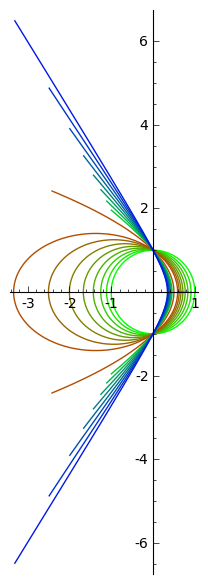
\includegraphics[scale=.5]{imagenes/conicas.png}

\end{frame}  

\begin{frame}[fragile]{Un poco de mecánica celeste}

Hemos logrado encontrar $r$ como función de $\theta$. Esto fue importante, de allí por ejemplo deducimos que las órbitas eran cónicas. No obstante
no hemos logrado resolver aún el problema de los dos cuerpos \eqref{eq:grav},  para ello deberíamos encontrar $\v{r}(t)$, es decir poner a $
\v{r}$ como función de $t$. Esto nos serviría para decir que punto de la órbita ocupa el planeta en unn dado momento.  Este problema no lo desarrollaremos aquí dado 
que su solución se aparte del tema de las ecuaciones diferenciales.
que excede los objetivos de este curso. 



\end{frame}  



\end{document}
%\documentclass{article}
%\documentclass[hyperref={colorlinks=true}]{beamer}
\documentclass[handout,hyperref={colorlinks=true}]{beamer}


%%%%%%%%%%%%%%%%%%%%%%%%%%%%%%Paquetes%%%%%%%%%%%%%%%%%%%%%%%%%%%%%%%%%%%%%%%%%%%%%%%5
%%%%%%%%%%%%%%%%%%%%%%%%%%%%%%%%%%%%%%%%%%%%%%%%%%%%%%%%%%%%%%%%%%%%%%%%%%%%%%%%%%%%%

\usepackage{pgfpages}
%\pgfpagesuselayout{2 on 1}[a4paper,border shrink=5mm]
\usepackage{empheq}
\usepackage[spanish]{babel}
\usepackage[utf8x]{inputenc}
\usepackage{times}
\usepackage[T1]{fontenc}
\usepackage{amssymb,amsmath}
\usepackage{enumerate}
\usepackage{verbatim}
\usepackage{ esint }
%\usepackage{pst-all}
%\usepackage{pstricks-add}
\usepackage{array}
%\usepackage[T1]{fontenc}
\usepackage{animate}
%\usepackage{media9}
\usepackage{xparse}
\usepackage{listings}
\usepackage{ wasysym }
\usepackage{sagetex}
\usepackage{hyperref}




%%%%%%%%%%%%%%%%%%%%%%%%%Configuracion listing
\lstdefinelanguage{Sage}[]{Python}
{morekeywords={False,sage,True},sensitive=true}
\lstset{
  frame=none,
  showtabs=False,
  showspaces=False,
  showstringspaces=False,
  commentstyle={\ttfamily\color{dgreencolor}},
  keywordstyle={\ttfamily\color{dbluecolor}\bfseries},
  stringstyle={\ttfamily\color{dgraycolor}\bfseries},
  language=Sage,
  basicstyle={\fontsize{8pt}{8pt}\ttfamily},
  aboveskip=.3em,
  belowskip=0.1em,
  numbers=none,
  numberstyle=\footnotesize
}


 


%%%%%%%%%%%%%%%%%%%%%%%%Colores
\definecolor{myblue}{rgb}{.8, .8, 1}
\definecolor{dblackcolor}{rgb}{0.0,0.0,0.0}
\definecolor{dbluecolor}{rgb}{0.01,0.02,0.7}
\definecolor{dgreencolor}{rgb}{0.2,0.4,0.0}
\definecolor{dgraycolor}{rgb}{0.30,0.3,0.30}
\newcommand{\dblue}{\color{dbluecolor}\bf}
\newcommand{\dred}{\color{dredcolor}\bf}
\newcommand{\dblack}{\color{dblackcolor}\bf}










%%%%%%%%%%%%%%%%%%%%%%%%%%Nuevos comandos entornos%%%%%%%%%%%%%%%%%%%%%%%%%%%%%%%%
%%%%%%%%%%%%%%%%%%%%%%%%%%%%%%%%%%%%%%%%%%%%%%%%%%%%%%%%%%%%%%%%%%%%%%%%
\newenvironment{demo}{\noindent\emph{Dem.}}{$\square$ \newline\vspace{5pt}}
\newcommand{\com}{\mathbb{C}}
\newcommand{\dis}{\mathbb{D}}
\newcommand{\rr}{\mathbb{R}}
\newcommand{\oo}{\mathcal{O}}
\renewcommand{\emph}[1]{\textcolor[rgb]{1,0,0}{#1}}
\newcommand{\der}[2]{\frac{\partial #1}{\partial #2}}
\renewcommand{\v}[1]{\overrightarrow{#1}}
\renewcommand{\epsilon}{\varepsilon}
\newlength\mytemplen
\newsavebox\mytempbox
\makeatletter
\newcommand\mybluebox{%
    \@ifnextchar[%]
       {\@mybluebox}%
       {\@mybluebox[0pt]}}

\def\@mybluebox[#1]{%
    \@ifnextchar[%]
       {\@@mybluebox[#1]}%
       {\@@mybluebox[#1][0pt]}}

\def\@@mybluebox[#1][#2]#3{
    \sbox\mytempbox{#3}%
    \mytemplen\ht\mytempbox
    \advance\mytemplen #1\relax
    \ht\mytempbox\mytemplen
    \mytemplen\dp\mytempbox
    \advance\mytemplen #2\relax
    \dp\mytempbox\mytemplen
    \colorbox{myblue}{\hspace{1em}\usebox{\mytempbox}\hspace{1em}}}

\makeatother
\DeclareDocumentCommand\boxedeq{ m g }{%
    {\begin{empheq}[box={\mybluebox[2pt][2pt]}]{equation}% #1%
        \IfNoValueF {#2} {\label{#2}}%
       #1
       \end{empheq}
    }%
}
\DeclareMathOperator{\atan2}{atan2}
\DeclareMathOperator{\sen}{sen}
\newtheorem{teorema}{Teorema}[section]
\newtheorem{lema}[teorema]{Lema}
\newtheorem{corolario}[teorema]{Corolario}
\newtheorem{proposicion}[teorema]{Proposici\'on}
\newtheorem{definicion}[teorema]{Definici\'on}
%%%%%%%%%%%%%%%%%%%%%%%%%%%%%%%%%%%%%%%%%%%%%%%%%%%%%%%%%%%%%%%%%%%%%%%%%%%%%%%%%%%%%%%%%%%%%%%%%%%%%%%%%%%




%%%%%%%%%%Para escibir en clase articulo o similar
% \usepackage{color}
% \newcommand{\nl}{ }
% \renewenvironment{frame}[1]{}{}
% \newcommand{\qed}{$\square$}
% %\newcommand{\defverbatim}{\def{#1}}
% \newenvironment{block}[1]{\textbf{#1}}{}
% \title{Ecuaciones lineales de segundo orden}
% \author{Fernando Mazzone}
% 




%%%%%%%%%%%%%%%%%%%%%%%Para clase beamer
\newcommand{\nl}{\onslide<+-> }
% \mode<all>
% {
%   \usetheme{Boadilla}
%   % oder ...
%  
%   \setbeamercovered{wolverine}
%   % oder auch nicht
% }


\mode<handout>{
  \usetheme{default}
  %\setbeamercolor{background canvas}{bg=black!5}
  \pgfpagesuselayout{4 on 1}[letterpaper,landscape,border shrink=2.5mm]
}

% \mode<all>{
%   \usetheme{default}
%   %\setbeamercolor{background canvas}{bg=black!5}
%   \pgfpagesuselayout{4 on 1}[letterpaper,landscape,border shrink=2.5mm]
% }

\title[Ecuaciones lineales de segundo orden] % (optional, nur bei langen Titeln nötig)
{%
 Ecuaciones lineales de segundo orden
}



\author[] % (optional, nur bei vielen Autoren)
{Fernando Mazzone}

\institute[Depto de Matemática] % (optional, aber oft nötig)
{
 Depto de Matemática\\
Facultad de Ciencias Exactas Físico-Químicas y Naturales\\
Universidad Nacional de Río Cuarto}


\subject{Ecuaciones Diferenciales}

%%%%%%%%%%%%%%%%%%%%%%%%%%%%%%%%%%%%%%%%%%%%%%%%%%%%%%%%%%%%%%%%%%%%%%%%%%%%%%%%%%%%%%




\begin{document}

\begin{frame}
\begin{block}{Ecuación lineal general de orden $n$}
Es una ecuación de la forma
\boxedeq{y^{(n)}(x)+p_{n-1}(x)y^{(n-1)}(x)+\cdots+p_1(x)y'(x)+p_0(x)y(x)=r(x)}{eq:ecua_lin_gen_orden_n}
donde $p_i,r$, $i=0,\ldots,n-1$ son funciones definidas en un intervalo $I$
\end{block}


Los resultados y técnicas que hemos desarollado para ecuaciones de orden $2$ se aplican con cambios menores a ecuaciones de mayor orden. No vamos a repetir la demostración de estos resultados, dados que es prácticamente la misma. Los exponemos de manera sumaria.
\end{frame}


\begin{block}{Teorema de existencia y unicidad de soluciones}
 Supongamos $p_i,r$, $i=0,\ldots,n-1$ continuas sobre $I$. Sean $x_0\in I$ e $y_0,y_1,\ldots y_{n-1}\in\rr$ dados. Entonces existe una única solución del PVI
 \[\left\{
 \begin{array}{l l l}
   y^{(n)}(x)+&p_{n-1}(x)y^{(n-1)}(x)+\cdots+p_0(x)y(x)=r(x),x\in I\\
   y(x_0)&=y_0&\\
   y'(x_0)&=y_1&\\
   &\vdots\\
  y^{(n-1)}(x_0)&=y_{n-1}&\\
  \end{array}\right.
\]

\end{block}

\end{document}


\documentclass{article}
%\documentclass[hyperref={colorlinks=true}]{beamer}
%\documentclass[handout,hyperref={colorlinks=true}]{beamer}


%%%%%%%%%%%%%%%%%%%%%%%%%%%%%%Paquetes%%%%%%%%%%%%%%%%%%%%%%%%%%%%%%%%%%%%%%%%%%%%%%%
%%%%%%%%%%%%%%%%%%%%%%%%%%%%%%%%%%%%%%%%%%%%%%%%%%%%%%%%%%%%%%%%%%%%%%%%%%%%%%%%%%%%%

%\usepackage{pgfpages}
%\pgfpagesuselayout{4 on 1}[a4paper,landscape,border srhrink=5mm]
\usepackage{empheq}
\usepackage[spanish]{babel}
\usepackage[utf8x]{inputenc}
\usepackage{times}
\usepackage[T1]{fontenc}
\usepackage{amssymb,amsmath}
\usepackage{enumerate}
\usepackage{verbatim}
\usepackage{ esint }
\usepackage{pdfsync}
%\usepackage{pst-all}
%\usepackage{pstricks-add}
\usepackage{array}
%\usepackage[T1]{fontenc}
\usepackage{animate}
%\usepackage{media9}
%\usepackage{movie15}
\usepackage{xparse}
\usepackage{listings}
\usepackage{ wasysym }
\usepackage{sagetex}
\usepackage{hyperref}
\usepackage{tabularx}
\usepackage{xcolor}
\usepackage{adjustbox}
\usepackage[spanish]{varioref}



%%%%%%%%%%%%%%%%%%%%%%%%%%Nuevos comandos entornos%%%%%%%%%%%%%%%%%%%%%%%%%%%%%%%%
%%%%%%%%%%%%%%%%%%%%%%%%%%%%%%%%%%%%%%%%%%%%%%%%%%%%%%%%%%%%%%%%%%%%%%%%
%%%%%%%%%%%%%%%%%%%%%%%%Colores

\definecolor{myblue}{rgb}{.8, .8, 1}
\definecolor{dblackcolor}{rgb}{0.0,0.0,0.0}
\definecolor{dbluecolor}{rgb}{0.01,0.02,0.7}
\definecolor{dgreencolor}{rgb}{0.2,0.4,0.0}
\definecolor{dgraycolor}{rgb}{0.30,0.3,0.30}
\definecolor{color_teor}{HTML}{FFFDA2}
\definecolor{color_ejer}{HTML}{F6BFBF}
\definecolor{color_cor}{HTML}{49E6D8}
\definecolor{color_lem}{HTML}{C6F6AB}
\definecolor{color_defi}{HTML}{EDA07C}
\newcommand{\dblue}{\color{dbluecolor}\bf}
\newcommand{\dred}{\color{dredcolor}\bf}
\newcommand{\dblack}{\color{dblackcolor}\bf}

%%%%%%%%%%%%%%%%%%%Teoremas, definiciones , etc

\newenvironment{demo}{\noindent\emph{Dem.}}{{\hspace*{\fill}$\square$} \newline\vspace{5pt}}
\newenvironment{colbox}[2]{%
    \begin{adjustbox}{minipage={\linewidth},margin=1ex,bgcolor=#1,env=center}
        #2}{%
    \end{adjustbox}%
}

\newcounter{defi_cont}
\newenvironment{definicion}[1]{\begin{colbox}{color_defi}{\refstepcounter{defi_cont}\textbf{Definición \arabic{defi_cont}.} #1}}{\end{colbox}}

\newcounter{teor_cont}
\newenvironment{teorema}[1]{\refstepcounter{teor_cont}\begin{colbox}{color_teor}{\textbf{Teorema \arabic{teor_cont}.} #1}}{\end{colbox}}

\newcounter{cor_cont}
\newenvironment{corolario}[1]{\begin{colbox}{color_cor}{\refstepcounter{cor_cont}\textbf{Corolario \arabic{cor_cont}.} #1}}{\end{colbox}}

\newcounter{lem_cont}
\newenvironment{lema}[1]{\begin{colbox}{color_lem}{\refstepcounter{lem_cont}\textbf{Lema \arabic{lem_cont}.} #1}}{\end{colbox}}

\newcounter{ejem_cont}
\newenvironment{ejemplo}[1]{\refstepcounter{ejem_cont}\vspace{1ex}\noindent\textbf{Ejemplo \arabic{ejem_cont}.} #1}{}

\newcounter{ejer_cont}
\newenvironment{ejercicio}[1]{\begin{colbox}{color_ejer}{\refstepcounter{ejer_cont}\textbf{Ejercicio \arabic{ejer_cont}.} #1}}{\end{colbox}}


%%%%%%%%%%%%%%%%%%%%%%%%%%%%%%%%%%%%Simbolos

\newcommand{\com}{\mathbb{R}}
\newcommand{\dis}{\mathbb{D}}
\newcommand{\rr}{\mathbb{R}}
\newcommand{\oo}{\mathcal{O}}
\renewcommand{\emph}[1]{\textcolor[rgb]{0,0,1}{#1}}
\newcommand{\der}[2]{\frac{\partial #1}{\partial #2}}
\renewcommand{\v}[1]{\overrightarrow{#1}}
\renewcommand{\epsilon}{\varepsilon}
\DeclareMathOperator{\mcd}{mcd}
\DeclareMathOperator{\atan2}{atan2}
\DeclareMathOperator{\sen}{sen}
%%%%%%%%%%%%%%%%%%%%%%%%%%%%%%Formulas en cajas 
\newlength\mytemplen
\newsavebox\mytempbox
\makeatletter
\newcommand\mybluebox{%
    \@ifnextchar[%]
       {\@mybluebox}%
       {\@mybluebox[0pt]}}

\def\@mybluebox[#1]{%
    \@ifnextchar[%]
       {\@@mybluebox[#1]}%
       {\@@mybluebox[#1][0pt]}}

\def\@@mybluebox[#1][#2]#3{
    \sbox\mytempbox{#3}%
    \mytemplen\ht\mytempbox
    \advance\mytemplen #1\relax
    \ht\mytempbox\mytemplen
    \mytemplen\dp\mytempbox
    \advance\mytemplen #2\relax
    \dp\mytempbox\mytemplen
    \colorbox{myblue}{\hspace{1em}\usebox{\mytempbox}\hspace{1em}}}

\makeatother
\DeclareDocumentCommand\boxedeq{ m g }{%
    {\begin{empheq}[box={\mybluebox[2pt][2pt]}]{equation}% #1%
        \IfNoValueF {#2} {\label{#2}}%
       #1
       \end{empheq}
    }%
}

%%%%%%%%%%%%%%%%%%%%%%%%%%%%%%%%%%%%%%%%%%%%%%%%%%%%%%%%%%%%%%%%%%%%%%%%%%%%%%%%%%%%%%%%%%%%%%%%%%%%%%%%%%%%%%%%%%%%%%%%%%%%%%%%%%%%%%%%%%%%%%%%%%%%%%%%%%%%%%%%%%%%%%%%%%%%%%%%%%%%%%%%%%%%%%%
\lstdefinelanguage{SymPy}[]{Python}
{morekeywords={False,sage,True,symbols,sympy,diff,solve,subs,factorial,expand},sensitive=true}
\lstset{
frame=none,
showtabs=False,
showspaces=False,
showstringspaces=False,
commentstyle={\ttfamily\color{dgreencolor}},
keywordstyle={\ttfamily\color{dbluecolor}\bfseries},
stringstyle={\ttfamily\color{dgraycolor}\bfseries},
language=SymPy,
basicstyle={\fontsize{8pt}{8pt}\ttfamily},
aboveskip=.3em,
belowskip=0.1em,
numbers=none,
numberstyle=\footnotesize
}







\begin{document}



 \section{Series de potencias}

En esta sección recordamos algunos conceptos y teoremas sobre series de potencias. Dado que este tema es motivo de un estudio más profundo en otras materias de la licenciatura en matemática omitimos algunas demostraciones.
\subsection{Definición} %Primer Frame para información personal.
\begin{definicion} Una serie de potencias es una serie de la forma:
\[
	\sum\limits_{n=0}^{\infty}a_n(z-z_0)^n
\]
donde $a_n$, $n=0,1,\ldots$, $z_0$ y $z$ son elementos de $\com$.
\end{definicion}


Estamos interesados en determinar los valores de $z$ para los cuales   una serie converge. 

\begin{ejemplo} La serie geométrica
\[
	\sum\limits_{n=0}^{\infty}z^n,
\]
es una serie de potencias. Aquí  $a_n=1$, $n=0,1,\ldots$ y $z_0=0$. Esta serie converge para $|z|<1$ a
\[ \frac{1}{1-z}\]
y no converge para cualquier otro valor de $z\in\com$.
\end{ejemplo}

\begin{ejemplo} Supongamos $f:I\to\rr$, donde $I$ es un intervalo abierto $I=(a,b)$ y que $f$ tiene derivadas de todo orden en  $z_0\in I$. Entonces es posible construir la serie de Taylor de $f$ en $z_0$ que es una serie de potencias. Recordemos que esta serie es
\[S(f,z_0,z)=\sum\limits_{n=0}^{\infty}\frac{f^{(n)}(z_0)}{n!}(z-z_0)^n.\]
\end{ejemplo}

 
 

\subsection{Límites superior e inferior}


\begin{definicion} Dada una sucesión de números reales $x_n$, 
 consideramos una nueva sucesión:

\[
	A_n=\sup\{x_n, x_{n+1},\ldots \}
\]

La nueva sucesión de reales $A_n$ es  no creciente ($A_n\geq A_{n+1}$), luego tiene un límite (puede ser $\pm\infty$). A este límite lo llamamos \emph{el límite superior de $x_n$}. Lo denotamos por $\limsup_{n\to\infty} x_n$. Es decir:   


\[
\limsup_{n\to\infty} x_n=\lim_{n\to\infty} A_n=\lim\limits_{n\to \infty} \sup\{x_n, x_{n+1},\ldots \}.
\]


Tomando ínfimo en lugar de supremo conseguimos \emph{el límite inferior} ($\liminf$).  
\end{definicion}
\begin{ejemplo}  Si $x_n=(-1)^n$, entonces
\[
	\{x_n,x_{n+1},\ldots\}=\{\pm1,\mp1,\pm1,\ldots\}.
\]
El supremo de este conjunto  es para todo $n$ igual a 1 y el ínfimo igual a -1. Luego $\liminf x_n=-1$ y $\limsup x_n=1$. 
\end{ejemplo}



\begin{ejemplo}  Si $x_n=1/n$, si $n$ es par y $x_n=1$ si $n$ es impar, entonces el conjunto

\[
	\{x_n,x_{n+1},\ldots\}
\]
tiene por supremo 1 y el ínfimo igual a $0$ . Luego $\liminf x_n=0$ y $\limsup x_n=1$. 
\end{ejemplo}

\begin{teorema}\textbf{Propiedades} Sea $x_n$  e $y_n$ dos sucesiones de números reales, entonces:

\begin{enumerate}
	\item El $\limsup x_n$ y el $\liminf x_n$  existen si se permite que $\pm\infty$ sean sus posibles valores.
	\item $\liminf x_n \leq \limsup x_n$.
	\item $\liminf x_n=\limsup x_n$ si y solo si el $\lim x_n$ existe. En este caso todos los límites coinciden.
	\item $\liminf (x_n+y_n)\geq \liminf x_n + \liminf y_n$.
	\item $\limsup (x_n+y_n)\leq \limsup x_n + \limsup y_n$

\end{enumerate}
\end{teorema}



\subsection{Radio de convergencia}


\begin{definicion} Dada la serie de potencias 
\[
	\sum\limits_{n=0}^{\infty}a_n(z-z_0)^n,
\]
definimos el \emph{radio de convergencia} $R$ de la siguiente forma:



\[
\frac{1}{R}=\limsup\limits_{n\to \infty} |a_n|^{1/n}.
\]

\end{definicion}

\begin{ejemplo} La serie  
\[
	\sum\limits_{n=0}^{\infty}z^n,
\]
tiene radio de convergencia:

\[\frac{1}{R}=\limsup\limits_{n\to \infty}1^{1/n}=\lim\limits_{n\to\infty}1^{1/n}=1\]
Luego $R=1$. 
\end{ejemplo}

\begin{ejemplo} La serie  
\[
	\sum\limits_{n=0}^{\infty}\bigg(\frac{1}{M}\bigg)^nz^n,
\]
tiene radio de convergencia:

\[\frac{1}{R}=\limsup\limits_{n\to \infty}\bigg(\bigg(\frac{1}{M}\bigg)^n\bigg)^{1/n}=\lim\limits_{n\to\infty}\bigg(\bigg(\frac{1}{M}\bigg)^n\bigg)^{1/n}=\frac1M\]
Luego $R=M$. 

\end{ejemplo}

\begin{ejemplo} Fijemos $M>0$ y $n$ un natural tal que $[n/2] >M$ (aquí $[x]$ es la parte entera de $x$). Entonces,
como $n-[n/2]\geq [n/2]>M$

\[ 
\begin{split}
n!=n(n-1)\cdots 1 &> n(n-1)\cdots (n-[n/2]) \\
&>\underbrace{M\cdots M }_{[n/2]-\hbox{veces}}\\
&\geq M^{[n/2]}\\
&> M^{n/3}\\
\end{split}
\]
Luego 
\[\frac{1}{R}:=\limsup_{n\to\infty} (1/n!)^{1/n}\leq \lim_{n\to\infty} \bigg(\frac{1}{M^{n/3}}\bigg)^{1/n}=\frac{1}{\sqrt[3]{M}}\]
Como $M$ es arbitrario, haciendo $M\to\infty$ vemos que el radio de convergencia de la serie  $\sum\limits_{n=0}^{\infty}\frac{1}{n!}z^n$ 
es $R=\infty$. 
\end{ejemplo}

\begin{teorema}  Supongamos que la serie:
\[
	\sum\limits_{n=0}^{\infty}a_n(z-z_0)^n,
\]
tiene radio de convergencia $R>0$. Entonces:
\begin{enumerate}
	\item Si $|z-z_0|<R$, la serie converge absolutamente en $z$. 
	\item Si $|z-z_0|>R$, la serie diverge.
	\item Si $|z-z_0|=R$, no se afirma nada.
	
\end{enumerate}
\end{teorema}
	
 \begin{demo} Se puede suponer sin perdida de generalidad $z_0=0$. Supongamos $0<R<\infty$.  Sea $L=1/R$ y tomemos $\epsilon>0$ pequeño. Como
\[\lim_{n\to\infty}\sup\{|a_n|^{1/n},|a_{n+1}|^{1/n+1},\ldots\}=L\]
para $n_0$ suficientemente grande
\[\sup\{|a_n|^{1/n},|a_{n+1}|^{1/n+1},\ldots\}<L+\epsilon.\]
para $n\geq n_0$.   Así
\[|a_n|^{1/n}<L+\epsilon\quad\hbox{para } n\geq n_0.\]
Elijamos $0<r<1/(L+\epsilon)<1/L=R$. Si $|z|<r$ entonces
\[|a_n||z|^n<(L+\epsilon)^nr^n\quad\hbox{para } n\geq n_0.\]
Pero $r(L+\epsilon)<1$. La desigualdad de arriba y el teorema de comparación para series (notar que el miembro de la derecha forma una serie geométrica) implican que la serie converge absolutamente para este $z$.  Esto implica la convergencia para cualquier $|z|<R$, ya que si $|z|<R=1/L$ existe $\epsilon>0$ lo suficientemente chico para que $|z|<1/(L+\epsilon)$. Por el resultado ya demostrado la serie converge absolutamente para este $z$.\end{demo}
\begin{ejercicio} Demostrar los casos $R=0$, $R=\infty$ y el segundo inciso.
 \end{ejercicio}
\begin{teorema}  La función
\[
f(z)=	\sum\limits_{n=0}^{\infty}a_n(z-z_0)^n,
\]
es diferenciable dentro en $\{z:|z-z_0|<R\}$. Además
\[
f'(z)=g(z):=	\sum\limits_{n=1}^{\infty}na_n(z-z_0)^{n-1},
\]
teniendo esta serie el mismo radio de convergencia que el de $f$.
\end{teorema}

\begin{demo} Nuevamente supondremos $z_0=0$. La afirmación sobre el radio de convergencia es consecuencia de que $\lim_{n\to\infty}n^{1/n}=1$. Como el radio $R'$ de convergencia de $g$ es:

\[
\begin{split}
\frac{1}{R'}&=\limsup_{n\to\infty}|a_{n+1}(n+1)|^{1/(n+1)}\\
&\underbrace{=}_{\hbox{\emph{ Ejercicio}}}\limsup_{n\to\infty}|a_{n+1}|^{1/(n+1)}\lim_{n\to\infty}|(n+1)|^{1/(n+1)}\\
&=\limsup_{n\to\infty}|a_{n+1}|^{1/(n+1)}=\frac{1}{R}
\end{split}\]

Ahora veamos que  $f'=g$.   Sea $0<r<R$, $|z_0|<r$ y $N\in\mathbb{N}$. Pongamos:
\[f(z)=S_N(z)+E_N(z),\]
\[S_N(z)=\sum_{n=0}^{N}a_nz^n\quad\hbox{y}\quad E_N(z)=\sum_{n=N+1}^{\infty}a_nz^n\]
Tomemos $|h|<r-|z_0|$, así $|z_0+h|<r$.  Tenemos
\[\begin{split}
\frac{f(z_0+h)-f(z_0)}{h}-g(z_0)&= \frac{S_N(z_0+h)-S_N(z_0)}{h}-S_N'(z_0)\\
				&+S_N'(z_0)-g(z_0)\\
				&+\frac{E_N(z_0+h)-E_N(z_0)}{h}
\end{split}\]

Ahora si $\epsilon>0$

\[\begin{split}
				&\bigg|\frac{E_N(z_0+h)-E_N(z_0)}{h}\bigg|\leq\sum_{n=N+1}^{\infty}|a_n|\bigg|\frac{(z_0+h)^n-z_0^n}{h}\bigg|\\
				&=\sum_{n=N+1}^{\infty}|a_n|(|z_0|^{n-1}+|z_0|^{n-2}h+\cdots+h^{n-1})\\
				&\leq2\sum_{n=N+1}^{\infty}|a_n|nr^{n-1}<\epsilon\\
\end{split}\]
Para $N$ suficientemente grande. Además como $S_N'(z)\to g(z)$ cuando $N\to\infty$ podemos elegir, a su vez, $N$ suficientemente grande para que

\[
	|S_N'(z_0)-g(z_0)|<\epsilon
\]

 Fijemos un $N$ que satisfaga las condiciones anteriores. Ahora podemos encontrar $\delta>0$ para que $|h|<\delta$ cumpla que 
\[
\bigg|\frac{S_N(z_0+h)-S_N(z_0)}{h}-S_N'(z_0)\bigg|<\epsilon.
\]

Esto muestra que $f'(z_0)=g(z_0)$ y por consiguiente $f$ es derivavble.  
\end{demo}


 


\begin{corolario}  Una serie de potencias es infinitamente diferenciable. Las sucesivas derivadas se obtienen derivando término a término la serie. El radio de convergencia se conserva.
\end{corolario}

\begin{ejemplo}  Hemos visto que la serie:
\[
	f(z)=\sum_{n=0}^{\infty}\frac{1}{n!}z^n
\]
tiene radio de convergencia infinito y por ende converge en $\com$. Ahora vemos que
\[f'(z)=\sum_{n=1}^{\infty}\frac{1}{(n-1)!}z^{n-1} =\sum_{n=0}^{\infty}\frac{1}{n!}z^n
\]
Lo que nos dice que $f$ resuelve la simple ecuación diferencial $f'(z)=f(z)$. La misma ecuación es resuelta por $g(z)=e^z$. Además $f(0)=g(0)=1$. Por el Teorema de existencia y unicidad $f(z)=g(z)$ para todo $z$. Hemos probado la importante fórmula.
\boxedeq{e^z=\sum_{n=0}^{\infty}\frac{1}{n!}z^n}{eq:exp}
\end{ejemplo}
\subsection{Funciones analíticas}
\begin{definicion} Una función $f:\Omega\subset\com\to\com$ se dirá analítica si para cada $z_0\in\Omega$, existe  $R>0$ y $a_n\in\com$, tal que:

\[ f(z)=\sum_{n=0}^{\infty}a_n(z-z_0)^n,\quad\hbox{para } |z-z_0|<R \]
\end{definicion}


\begin{ejercicio} Si $f$ es analítica tenemos la siguiente fórmula
\[
	a_n=\frac{f^{(n)}(z_0)}{n!}
\]
para los coeficientes $a_n$. 
\end{ejercicio}

 \begin{teorema}\label{teor_oper_series}\textbf{Operaciones entre series de potencias} Supongamos que $f(z)=\sum_{n=0}^{\infty}a_n(z-z_0)^n$ y  $g(z)=\sum_{n=0}^{\infty}b_n(z-z_0)^n$ son series de potencias con radio de convergencia mayor o igual a $R>0$. Entonces $f+g$ y $fg$ son funciones analíticas que tienen por desarrollo en serie
\[
    \begin{split}
      (f+g)(z)&=\sum_{n=0}^{\infty}(a_n+b_n)(z-z_0)^n\\
      (fg)(z)&=\sum_{n=0}^{\infty}\left(\sum_{k=0}^na_kb_{n-k}\right)(z-z_0)^n,\\
    \end{split}
\]
y los radios de convergencia de las series anteriores es, al menos, $R$. Si $g(z)\neq 0$ para $|z-z_0|<R$ entonces $f(z)/g(z)$ es analítica y se desarrolla por  una  serie de radio de convergencia al menos $R$. Es posible expresar los coeficientes del cociente en términos de los coeficientes del dividendo y divisor, pero no nos detendremos en ello.   
\end{teorema}


\section{Solución de EDO mediante series de potencias. Método coeficientes indeterminados}



\subsection{Método coeficientes indeterminados}

Dada una EDO

\begin{equation} \hbox{(1)}\quad  F(x,y,y',\ldots,y^{(n)})=0\end{equation}
queremos desarrollar en series de potencias  la solución general a esta ecuación. El método que estudiaremos se denomina \emph{metodo de los coeficientes indeterminados}. Consiste en proponer el desarrollo en serie de la solución

\[y(x)=a_0+a_1(x-x_0)+a_2(x-x_0)^2+\cdots  \]
remplazar $y(x)$ por este desarrollo en  en la ecuación (1) y tratar de resolver la ecuación resultante para los coeficientes (indeterminados) $a_n$. El método suele funcionar en algunas ecuaciones. Desarrollemos un ejemplo.

 

\begin{ejemplo} Hallar el desarrollo en serie de la solución del siguiente pvi 
\[\left\{\begin{array}{l l} y'&=y\\ y(0)&=1\end{array}\right.\]
La solución, es bien sabido, es $y(x)=e^x$,  pero pretendemos reencontrarla por el método expuesto. Escribimos
\[\begin{split}
   y&=a_0+a_1x+a_2x^2+\cdots+a_nx^n+\cdots\\
   y'&=a_1+2a_2x+3a_3x²+\cdots+(n+1)a_{n+1}x^n+\cdots
  \end{split}
\]
La igualdad $y'=y$ implica que 
\[\begin{split}
   a_1&=a_0\\
   a_2&=\frac{a_1}{2}\\
   a_3&=\frac{a_2}{3}\\
      &\,\,\,\,\vdots \\
   a_{n+1}&=\frac{a_{n}}{n+1}
 \end{split}
\]
Si iteramos la fórmula $a_{n+1}=a_{n}/(n+1)$, obtenemos 
\[a_n=\frac{1}{n}a_{n-1}=\frac{1}{n(n-1)}a_{n-2}=\cdots=\frac{1}{n(n-1)\cdots 1}a_{0}=\frac{a_0}{n!}.\]
Pero $a_0=y(0)=1$. Luego 
\boxedeq{a_n=\frac{1}{n!}}{eq:exp}




\begin{lstlisting}
>>> from sympy import *
>>> Lista=['a%s'%i for i in range(orden)]
>>> Lista
['a0', 'a1', 'a2', 'a3', 'a4', 'a5', 'a6']
>>> x=symbols('x')
>>> a=symbols(Lista)
>>> y=sum([a[i]*x**i for i in range(orden)])
>>> y
a0 + a1*x + a2*x**2 + a3*x**3 + a4*x**4 + a5*x**5 + a6*x**6
>>> Ecua=y.diff(x)-y
>>> Ecua
-a0 - a1*x + a1 - a2*x**2 + 2*a2*x - a3*x**3 + 3*a3*x**2 - a4*x**4 + 4*a4*x**3 - a5*x**5 + 5*a5*x**4 - a6*x**6 + 6*a6*x**5
>>> Ecuaciones=[Ecua.coeff(x**i) for i in range(orden)]
>>> Ecuaciones
[a1, -a1 + 2*a2, -a2 + 3*a3, -a3 + 4*a4, -a4 + 5*a5, -a5 + 6*a6, -a6]
>>> Ecuaciones=[a[0]-1,Ecua.subs(x,0)]+Ecuaciones[1:-1]
>>> Ecuaciones
[a0 - 1, -a0 + a1, -a1 + 2*a2, -a2 + 3*a3, -a3 + 4*a4, -a4 + 5*a5, -a5 + 6*a6]
>>> coef=solve(Ecuaciones,Lista)
>>> coef
{a1: 1, a5: 1/120, a2: 1/2, a6: 1/720, a3: 1/6, a0: 1, a4: 1/24}
>>> y.subs(coef)
x**6/720 + x**5/120 + x**4/24 + x**3/6 + x**2/2 + x + 1
\end{lstlisting}


Vemos que la solución es 
\boxedeq{y(x)=1+x+\frac{x^2}{2}+\frac{x^3}{6}+\frac{x^4}{24}+\frac{x^5}{120}+\frac{x^6}{720} +\cdots         }{eq:sol_sage} 
\end{ejemplo}






\subsection{Relaciones de recurrencia}

La expresión $a_{n+1}=\frac{a_{n}}{n+1}$ es un ejemplo de \href{http://es.wikipedia.org/wiki/Relación_de_recurrencia}{relación de recurrencia}.
\begin{definicion} Una  relación de recurrencia para una sucesión $b_n$ de números reales es una sucesión de 
funciones $f_n:\rr^n\to\rr$ que relaciona $b_{n+1}$ con los términos anteriores de la sucesión por medio de 
la expresión
\begin{equation}\label{eq:recu} b_{n+1}=f_n(b_1,\ldots,b_n).
\end{equation}
Resolver una relación de recurrencia es encontrar una fórmula explícita de $b_n$ como función de $n$.
 \end{definicion}


Hay técnicas y métodos para resolver relaciones de recurrencia que guardan analogías con técnicas y métodos de resolver ecuaciones diferenciales.  No vamos a desarrollar este importante tema en este curso, sugerimos la \href{http://es.wikipedia.org/wiki/Relación_de_recurrencia}{correspondiente wiki} en la wikipedia. Sólo agregamos que  SymPy resuelve relaciones recurrentes a través del comando \texttt{rsolve}. 

\begin{ejemplo} Resolvamos con SymPy la sucesión de Fibonacci $a_{n+2}=a_{n+1}+a_n$.
\begin{lstlisting}
>>> from sympy import *
>>> n=symbols('n',integer=True)
>>> y = Function('y')
>>> f=Equality(y(n),y(n-1)+y(n-2))
>>> rsolve(f,y(n))
\end{lstlisting}

 El resultado es
 \boxedeq{a_n=C_0\left(\frac12+\frac{\sqrt{5}}{2}\right)^n +
 C_1\left(\frac12-\frac{\sqrt{5}}{2}\right)^n  }{}
Las constantes arbitrarias $C_0$ y $C_1$ aparecen porque una relación de recurrencia no tiene una única solución. Se dice que una relación de recurrencia tiene orden $k$ o es de $k$-términos si el coeficiente $a_n$ se expresa en función de los $k$  anteriores. En general la solución general de una relación de recurrencia de $k$-términos tiene $k$ constantes arbitrarias. Por consiguiente, si queremos una única solución debemos tener $k$ relaciones extras. Usualmente esto se consigue dando los valores de los $k$-primeros términos $a_0,\ldots,a_k$. Por ejemplo, en  la sucesión de Fibonacci si pedimos $a_0=a_1=1$.

\begin{lstlisting}
>>> C0,C1=symbols('C0,C1')
>>> A=C0*(1/2+sqrt(5)/2)**n+C1*(1/2-sqrt(5)/2)**n
>>> Cval=solve([A.subs(n,0)-1,A.subs(n,1)-1],[C0,C1])
>>> Fib=A.subs(Cval)
>>> [Fib.subs(n,i).expand() for i in range(10)]
[1, 1, 5/4, 5/4, 25/16, 25/16, 125/64, 125/64, 625/256, 625/256]
\end{lstlisting}
Llegamos a la fórmula
\boxedeq{a_n
\frac{1}{10} \, \left(\frac{1}{2} \, \sqrt{5}\right)^{n} {\left(2 \, \sqrt{5} + 5\right)} - \frac{1}{10} \, \left(-\frac{1}{2} \, \sqrt{5}\right)^{n} {\left(2 \, \sqrt{5} - 5\right)}
}{}

\end{ejemplo}

\subsection{Serie binomial}

 Se puede utilizar el método de coeficientes indeterminados para encontrar desarrollos en serie de una función  $f$. La técnica consiste en encontrar un pvi que satisfaga $f$ y le aplicamos el método de coeficientes indeterminados a ese pvi.

\begin{ejemplo}  Encontrar el desarrollo en serie de la función
\[y(x)=(1+x)^p\quad p\in\rr\]
La función $y(x)$ resuelve el pvi  $(1+x)y'(x)=py$, $y(0)=1$. apliquemos el método de coeficientes indeterminados a este pvi.
Como
\[\begin{split}
   y&=a_0+a_1x+a_2x^2+\cdots+a_nx^n+\cdots\\
   y'&=a_1+2a_2x+3a_3x²+\cdots+(n+1)a_{n+1}x^n+\cdots
  \end{split}
\]
Tenemos
\[\begin{split}
   py=&pa_0+pa_1x+pa_2x^2+\cdots+pa_nx^n+\cdots\\
  (1+x)y'=&a_1+2a_2x+3a_3x²+\cdots+(n+1)a_{n+1}x^n+\cdots\\
          &+a_1x+2a_2x^2+3a_3x³+\cdots+na_{n}x^n+\cdots\\
-------&----------------------\\
0=(1+x)y'-py =& (a_1-pa_0)+(a_1+2a_2-pa_1)x+\cdots +((n+1)a_{n+1}+na_n-pa_n)x^n+\cdots
  \end{split}
\]
Tenemos la relación
\[ a_{n+1}=\frac{(p-n)}{n+1}a_n.
\]
Que es una relación de recurrencia de un sólo término. Estas relaciones se resuelven iterando la relación de manera sucesiva de modo de relacionar $a_n$ con $a_0$
\[a_n=\frac{(p-n+1)}{n}a_{n-1}=\frac{(p-n+1)(p-n+2)}{n(n-1)}a_{n-2}=\cdots=\frac{(p-n+1)(p-n+2)\cdots p}{n!}a_0.\]
Como $a_0=y(0)=1$ vemos que
\boxedeq{a_n=\frac{(p-n+1)(p-n+2)\cdots p}{n!}.}{eq:coef_bin}
Si $p\in\mathbb{N}$ entonces $a_n=0$ para $n>p$. Esto es claro, por otro lado, ya que en este caso $(1+x)^p$ es un polinomio. Por la fórmula del binomio de Newton los coeficientes para $p\in \mathbb{N}$  no son más que los coeficientes binomiales
\[a_n=\binom{p}{n}\]
 Cuando $p\in\mathbb{R}$ aún vamos a seguir denominado a $a_n$, dado por la fórmula \eqref{eq:coef_bin},   coeficiente binomial. La serie resultante se llama la serie binomial. Cuando $p\in\mathbb{R}-\mathbb{N}$ es una serie infinita y no  un polinomio. Notar que para $p$ no entero positivo
\[\lim\limits_{n\to\infty}\frac{|a_{n+1}|}{|a_n|}=\lim\limits_{n\to\infty}\frac{|p-n|}{|n+1|}=1\]
Luego la serie tiene radio de convergencia 1.  Hemos demostrado asi que vale la siguiente fórmula, que es una generalización de la fórmula binomial de Newton
\boxedeq{(1+x)^p=1+px+\frac{p(p-1)}{2!}x^2  +\cdots=1+\binom{p}{1}x+\binom{p}{2}x^2+\cdots}{}
Esta importante serie se denomina \href{http://en.wikipedia.org/wiki/Binomial_series}{serie binomial}.


\begin{lstlisting}
>>> from sympy import *
>>> orden=4
>>> Lista=['a%s'%i for i in range(orden)]
>>> a=symbols(Lista)
>>> a
[a0, a1, a2, a3]
>>> x,p=symbols('x,p')
>>> y=sum([a[i]*x**i for i in range(orden)])
>>> y
a0 + a1*x + a2*x**2 + a3*x**3
>>> Ecua=(1+x)*y.diff(x)-p*y
>>> Ecua=Ecua.expand()
>>> Ecua
-a0*p - a1*p*x + a1*x + a1 - a2*p*x**2 + 2*a2*x**2 + 2*a2*x - a3*p*x**3 + 3*a3*x**3 + 3*a3*x**2
>>> Ecuaciones=[Ecua.diff(x,i).subs(x,0)/factorial(i) for i in range(orden)]
>>> Ecuaciones
[-a0*p + a1, -a1*p + a1 + 2*a2, -a2*p + 2*a2 + 3*a3, a3*(-p + 3)]
>>> Ecuaciones=[a[0]-1]+Ecuaciones[:-1]
>>> Sol_a_n=solve(Ecuaciones,a)
>>> Sol_a_n
{a3: p*(p - 2)*(p - 1)/6, a0: 1, a2: p*(p - 1)/2, a1: p}
>>> y.subs(Sol_a_n)
p*x**3*(p - 2)*(p - 1)/6 + p*x**2*(p - 1)/2 + p*x + 1
\end{lstlisting}



\boxedeq{y(x)=\frac{1}{6} \, {\left(p - 1\right)} {\left(p - 2\right)} p x^{3} + \frac{1}{2} \, {\left(p - 1\right)} p x^{2} + p x + 1}{}

\end{ejemplo}

\subsection{Oscilador armónico}

\begin{ejemplo} Consideremos la ecuación 
\[y''+\omega^2y=0.\]
Esta es una ecuación de segundo orden. Veamos si el método de coeficientes indeterminados nos lleva a la solución. Se tiene
\[\begin{split}
    \omega^2y&=\omega^2a_0+\omega^2a_1x+\omega^2a_2x^2+\cdots+\omega^2a_nx^n+\cdots\\
  y''&=2a_2+2\cdot 3a_3x+\cdots+(n+1)(n+2)a_{n+2}x^n+\cdots\\
--&---------------------------\\
0=y''+\omega^2y =& (\omega^2a_0+2a_2)+(\omega^2a_1+2\cdot 3a_3)x+\cdots +(\omega^2a_n+(n+1)(n+2)a_{n+2})x^n+\cdots
  \end{split}
\]
Encontramos la relación de recurrencia de dos términos
\boxedeq{a_{n+2}=-\frac{\omega^2a_n}{(n+1)(n+2)}.}{}
Notar que  en este caso $a_1$ y, obviamente, $a_0$ no se relacionan con ningún coeficiente anterior. Por este motivo es de esperar que podamos elegir de manera arbitraria $a_0$ y $a_1$. Esto está de acuerdo con el hecho que remarcamos antes de que en una relación de recurrencia de dos términos aparecen dos constantes arbitrarias y también está de acuerdo con que la solución general de una ecuación de segundo orden tiene dos constantes arbitrarias. En este caso resolvemos la relación de recurrencia relacionando $a_n$ con $a_0$ cuando $n$ es impar y con $a_1$ cuando es impar. Concretamente si $n=2k$, $k\in\mathbb{N}$,
\[a_{2k}=-\frac{\omega^2}{2k(2k-2)}a_{2k-2}=\cdots=(-1)^k\frac{\omega^{2k}}{(2k)!}a_0.\]
En cambio si $n=2k+1$ es impar
\[a_{2k+1}=-\frac{\omega^2}{(2k+1)2k}a_{2k-1}=\cdots=(-1)^k\frac{\omega^{2k}}{(2k+1)!}a_1.\]
Agrupando los términos pares y los impares de la serie de potencias resultante queda
\boxedeq{
   \begin{split}
     y(x) &=a_0\sum_{k=0}^{\infty}(-1)^k\frac{1}{(2k)!}\left(\omega x\right)^{2k}+\frac{a_1}{\omega}\sum_{k=0}^{\infty}(-1)^k\frac{1}{(2k+1)!}\left(\omega x\right)^{2k+1}\\
&=a_0\cos\omega x+\frac{a_1}{\omega}\sen\omega x
   \end{split}
 }{}
La última igualdad es conocida de las asignaturas de análisis. Es facil verificar, lo dejamos de ejercicio, que las series involucradas tienen radio de convergencia infinito.

Podemos hacer los cálculos anteriores con SAGE

\begin{lstlisting}
>>> from sympy import *
>>> orden=10
>>> Lista=['a%s'%i for i in range(orden)]
>>> a=symbols(Lista)
>>> x,omega=symbols('x,omega')
>>> y=sum([a[i]*x**i for i in range(orden)])
>>> Ecua=y.diff(x,2)+omega**2*y
>>> Ecuaciones=[Ecua.diff(x,i).subs(x,0)/factorial(i) for i in range(orden)]
>>> Ecuaciones_a=[a[0]-1,a[1]]+Ecuaciones[:-2]
>>> Sol_a_n=solve(Ecuaciones_a,a)
>>> y.subs(Sol_a_n)
omega**8*x**8/40320 - omega**6*x**6/720 + omega**4*x**4/24 - omega**2*x**2/2 + 1
>>> Ecuaciones_b=[a[0],a[1]-1]+Ecuaciones[:-2]
>>> Sol_a_n=solve(Ecuaciones_b,a)
>>> y.subs(Sol_a_n)
omega**8*x**9/362880 - omega**6*x**7/5040 + omega**4*x**5/120 - omega**2*x**3/6 + x
\end{lstlisting}



 Obtenemos las soluciones
\[
    \begin{split}
      y_1(x)&=\cdots+\frac{\omega^{8} x^{8}}{40320} - \frac{\omega^{6} x^{6}}{720} + \frac{\omega^{4} x^{4}}{24} - \frac{\omega^{2} x^{2}}{2} + 1
=\cos(\omega x)\\
      y_2(x)&=\cdots+\frac{\omega^{8} x^{9}}{362880} - \frac{\omega^{6} x^{7}}{5040} + \frac{\omega^{4} x^{5}}{120} - \frac{\omega^{2} x^{3}}{6} + x=\frac{1}{\omega}\sen\omega x\\
    \end{split}
\]
\end{ejemplo}

\subsection{Ecuación de Legendre. Primera aproximación}

\begin{ejemplo} Consideremos la \href{http://es.wikipedia.org/wiki/Polinomios_de_Legendre}{ecuación de Legendre}.
\boxedeq{(1-x^2)y''-2xy'+p(p+1)y=0,}{eq:ecua_lege}
donde $p>0$. Esta ecuación aparece en muchas aplicaciones, por ejemplo en muchos problemas que involucran funciones definidas en esferas, como es el caso de los modos normales de vibración de una esfera y en problemas de potenciales esféricos

\[\begin{split}
   p(p+1)y= p(p+1)&a_0+ p(p+1)a_1x+ p(p+1)a_2x^2+\cdots+ p(p+1)a_nx^n+\cdots\\
  -2xy'=&-2a_1x-4a_2x^2-6a_3x^3+\cdots-2na_{n}x^n+\cdots\\
(1-x^2)y''=& 2a_2+2\cdot 3a_3x+\cdots +(n+1)(n+2)a_{n+2}x^n+\cdots\\
          &-2a_2x^2-2\cdot 3a_3x^3-\cdots -(n-1)na_{n}x^n-\cdots\\
     -------&----------------------\\
0=(1-x^2)y''-2xy+p(p+1)y =& (p(p+1)a_0+2a_2)+(p(p+1)a_1-2a_12\cdot 3a_3)x+\cdots\\
     &+ \left( (p(p+1)-n(n+1)\right)a_n+n(n+1)a_{n+2})x^n+\cdots
  \end{split}
\]
Obtenemos la relación de recurrencia
\boxedeq{a_{n+2}=-\frac{(p-n)(p+n+1)}{(n+1)(n+2)} a_n}{eq:leg_rel_recu}
 Ahora vamos a dividir la serie en los términos pares e impares
\[\sum\limits_{n=0}^{\infty}a_nx^n= \sum\limits_{k=0}^{\infty}a_{2k}x^{2k}+\sum\limits_{k=0}^{\infty}a_{2k+1}x^{2k+1}\]
A cada una de estas series le podemos aplicar el criterio de la razón usando la fórmula de recuerrencia de arriba. Por ejemplo para los términos pares
\[\lim\limits_{k\to\infty}\frac{|a_{2k+2}x^{2k+2}|}{|a_{2k}x^{2k}|}=\lim\limits_{k\to\infty}\frac{|p_0-2k||p_0+2k+1|}{(2k+1)(2k+2)}|x|^2=|x|^2\]
De modo que la serie tiene radio de convergencia 1. La misma situación ocurre con la serie de términos impares. Esto muestra que la serie en su conjunto tambien tiene radio de convergencia igual a 1. Era previsible que el radio de convergencia no fuese mayor a 1, pues la forma explícita de la ecuación de la ecuación de Legendre es
\[y''-\frac{2x}{(1-x^2)}y'+\frac{p(p+1)}{(1-x^2)}y=0.\]
Se observa que $1$ y $-1$ son puntos singulares de la ecuación.

Podemos relacionar cualquier coeficiente de índice par $a_{2k}$ con el $a_0$ y cualquiera con índice impar $a_{2k+1}$ con el $a_1$. Esto lo resolveremos con SymPy

\begin{lstlisting}
>>> from sympy import *
>>> orden=10
>>> Lista=['a%s'%i for i in range(orden)]
>>> a=symbols(Lista)
>>> x,p=symbols('x,p')
>>> y=sum([a[i]*x**i for i in range(orden)])
>>> Ecua=(1-x**2)*y.diff(x,2)-2*x*y.diff(x)+p*(p+1)*y
>>> Ecuaciones=[Ecua.diff(x,i).subs(x,0)/factorial(i) for i in range(orden)]
>>> for ec in Ecuaciones:
...     ec
... 
a0*p*(p + 1) + 2*a2
a1*p*(p + 1) - 2*a1 + 6*a3
a2*p*(p + 1) - 6*a2 + 12*a4
a3*p*(p + 1) - 12*a3 + 20*a5
a4*p*(p + 1) - 20*a4 + 30*a6
a5*p*(p + 1) - 30*a5 + 42*a7
a6*p*(p + 1) - 42*a6 + 56*a8
a7*p*(p + 1) - 56*a7 + 72*a9
a8*p*(p + 1) - 72*a8
a9*(p*(p + 1) - 90)
>>> Sol_a_n=solve(Ecuaciones[:-2],a[2:])
>>> for sol in a[2:]:
...     Sol_a_n[sol].factor()
... 
-a0*p*(p + 1)/2
-a1*(p - 1)*(p + 2)/6
a0*p*(p - 2)*(p + 1)*(p + 3)/24
a1*(p - 3)*(p - 1)*(p + 2)*(p + 4)/120
-a0*p*(p - 4)*(p - 2)*(p + 1)*(p + 3)*(p + 5)/720
-a1*(p - 5)*(p - 3)*(p - 1)*(p + 2)*(p + 4)*(p + 6)/5040
a0*p*(p - 6)*(p - 4)*(p - 2)*(p + 1)*(p + 3)*(p + 5)*(p + 7)/40320
a1*(p - 7)*(p - 5)*(p - 3)*(p - 1)*(p + 2)*(p + 4)*(p + 6)*(p + 8)/362880

\end{lstlisting}





En general 
\[a_{2n}=\frac{(p+1)(p_0+3)\cdots (p+2n-1) \times p(p-2)\cdots (p-2n+2)}{(2n)!}a_0\]
y
\[a_{2n+1}=\frac{(p+2)(p+4)\cdots (p+2n) \times (p-1)(p-3)\cdots (p-2n+1)}{(2n+1)!}a_1\]
Podemos elegir $a_0$ y $a_1$ de manera arbitraria (esto está de acuerdo con que en una ecuación de orden 2 aparece 2 constantes de integración) y por las relaciones anteriores deducir el valor de los restantes $a_n$.

Un caso especial se plantea cuando  $p\in\mathbb{N}$. En esa situación vemos que infinitos de los $a_n$ resultan iguales a cero. De hecho una de las series, la de términos impares o la de términos pares acorde a que $p$ sea par o impar respectivamente,  se trunca. Supongamos que esto ocurre con la serie de términos impares, es decir $p$ es entero positivo impar. Si ahora tomamos $a_0=0$ toda la serie de términos pares se hará cero. Para $a_1$ elijo algún valor no nulo y esto me garantiza que los términos impares son no nulos hasta el término $a_{n}$, pero a partir de allí también se hacen cero. Es usual elegir $a_1$ para que $y(1)=1$. Nos queda definida así una función polinómica que se denomina \href{http://es.wikipedia.org/wiki/Polinomios_de_Legendre}{polinomio de Legendre} y se denota por $P_p$. Cuando $p$ es par hacemos una construcción análoga, quedando un polinomio $P_p$, con todas potencias pares, tal que $P_p(1)=1$.

Todos estos cálculos los programamos en la siguiente función de SymPy. Esta función tiene un argumento $n$ que debe ser un número natural y devuelve el correspondiente polinomio de Legendre.


\begin{lstlisting}
from sympy import *
def Legendre(n):
    orden=n+2
    Lista=['a%s'%i for i in range(orden)]
    a=symbols(Lista)
    x,p=symbols('x,p')
    y=sum([a[i]*x**i for i in range(orden)])
    Ecua=(1-x**2)*y.diff(x,2)-2*x*y.diff(x)+n*(n+1)*y
    Ecuaciones=[Ecua.diff(x,i).subs(x,0)/factorial(i) for i in range(orden-2)]       
    s=symbols('s')
    if n%2==0:
        Ecuaciones+=[a[0]-s,a[1]]
    else:
        Ecuaciones+=[a[0],a[1]-s]
    Sol_a_n=solve(Ecuaciones,a)
    y=y.subs(Sol_a_n)
    sol=solve(y.subs(x,1)-1,s)
    return y.subs(s,sol[0])
\end{lstlisting}

Esto es una función de Python. Se pueden copiar las lineas de arriba en una consola de Python, pero lo más usual es preparar un archivo aparte que luego se carga en una sesión de SymPy.  Las sentencias para cargar el archivo son las dadas aquí debajo, donde hemos supuesto que el archivo se llama \texttt{legendre.py} y esta en el directorio \texttt{/home/fdmazzone/Git/Ecuaciones\_Diferenciales/scripts}

\begin{lstlisting}
>>> import os
>>> os.chdir('/home/fdmazzone/Git/Ecuaciones_Diferenciales/scripts')
>>> from legendre import Legendre
\end{lstlisting}


Con la ayuda de esta función podemos generar rápidamente una tabla de polinomios de Legendre
\begin{lstlisting}
>>> for n in range(1,6):
...     Legendre(n)
... 
x
3*x**2/2 - 1/2
5*x**3/2 - 3*x/2
35*x**4/8 - 15*x**2/4 + 3/8
63*x**5/8 - 35*x**3/4 + 15*x/8
\end{lstlisting}
y graficarlos
\begin{lstlisting}
>>> for n in range(2,8):
...     p1=plot(Legendre(n),(x,-1,1),show=False)
...     p.append(p1[0])
... 
>>> p.show()
\end{lstlisting}


\begin{figure}[h]
\begin{center}
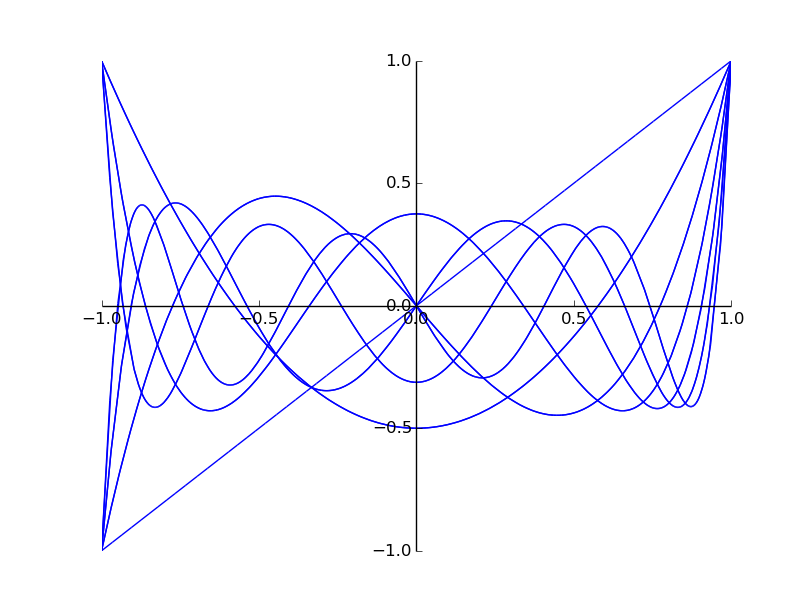
\includegraphics[scale=.25]{imagenes/legendre.png}
\caption{Polinomios de Legendre hasta el orden 8}
\end{center}
\end{figure}



\end{ejemplo}

\section{Teorema fundamental sobre puntos ordinarios}


\begin{definicion} Dada la ecuación diferencial
\[y''(x)+p(x)y'(x)+q(x)y(x)=0\]
donde $p,q$ son funciones   definidas en algún intervalo abierto $I$, diremos que $x_0\in I$ es un \emph{punto ordinario} de la ecuación si $p$ y $q$ son analíticas en $x_0$. Un punto no ordinario se llama \emph{singular}.
\end{definicion}

\begin{ejemplo} En la ecuación del oscilador armónico
\[y''+\omega^2 y=0 \]
todo punto es ordinario. 
\end{ejemplo}

\begin{ejemplo} En la ecuación de Legendre
\[(1-x^2)y''-2xy'+p(p+1)y=0 \]
$1$ y $-1$ son puntos singulares, otros valores de $x$ son puntos ordinarios. 
\end{ejemplo}

Antes de ir al Teorema más importante de esta sección vamos a enunciar un  lema que nos resultará útil.

\begin{lema}\label{lema:comp_recu}\textbf{Comparación.} Supongamos que tenemos una relación de recurrencia 
 \begin{equation}\label{eq:recu2} a_{n}=f_n(a_0,\ldots,a_{n-1})\quad n\geq 2\end{equation}
donde las funciones $f_n$ son crecientes respecto a sus todas las variables. Si la sucesión  $\{a_n\}$ resuelve \eqref{eq:recu2}, la sucesión  $\{b_n\}$ resuelve la desigualdad
 \[b_{n}\leq f_n(b_0,\ldots,b_{n-1})\quad n\geq 2 \]
y además vale que  $b_0\leq a_0$ y $b_1\leq a_1$, entonces $b_n\leq a_n$ para todo $n=2,3,\ldots$. En particular la afirmación se satisface cuando $f_n$ es lineal con coeficientes positivos, es decir $f_n(a_0,\ldots,a_{n-1})=\sum_{k=0}^{n-1}\alpha^n_ka_k$, con $\alpha^n_k\geq 0$ para $k=0,\ldots,n-1$.
\end{lema}
\begin{demo}
Es muy sencilla y la dejamos de ejercicio (evidentemenete hay que utilizar el principio de inducción). 
\end{demo}


\begin{teorema}\textbf{Teorema Fundamental Sobre Puntos Ordinarios.}\label{eq:teor_ptos_ord} Sea $x_0$ un punto ordinario de la ecuación
\[y''(x)+p(x)y'(x)+q(x)y(x)=0\]
y sean $a_0,a_1\in\mathbb{R}$. Existe una solución de la ecuación que es analítica en un entorno de $x_0$ y que satisface $y(x_0)=a_0$ e $y'(x_0)=a_1$. El radio de convergencia del desarrollo en serie de $y$ es al menos tan grande como el mínimo de los radios de convergencia de los desarrollos en serie de $p$ y $q$.
\end{teorema}

\begin{demo}
Supongamos, sin perder generalidad, que $x_0=0$. Consideremos que los desarrollos en serie de potencias de $p$ y $q$.
\begin{equation}\label{eq:series_p_q}p(x)=\sum_{n=0}^{\infty}p_nx^n\quad\text{y}\quad q(x)=\sum_{n=0}^{\infty}q_nx^n.
\end{equation}
Supongamos que ambas series convergen en $|x|<R$, para cierto $R>0$. Vamos a aplicar el método de coeficientes indeterminados. Tenemos
\[
    \begin{split}
      y&=\sum_{n=0}^{\infty}a_nx^n=a_0+a_1x+\cdots+a_nx^n+\cdots\\
      y'&=\sum_{n=0}^{\infty}(n+1)a_{n+1}x^n=a_1+2a_2x+\cdots+(n+1)a_{n+1}x^n+\cdots\\
      y''&=\sum_{n=0}^{\infty}(n+1)(n+2)a_{n+2}x^n= 2a_2+2\cdot 3a_3x+\cdots+(n+1)(n+2)a_{n+2}x^n+\cdots.
    \end{split}
\]
Por el  Teorema \ref{teor_oper_series} 
\[
   \begin{split}
     q(x)y&=\left(\sum_{n=0}^{\infty}a_nx^n\right)\left(\sum_{n=0}^{\infty}q_nx^n\right)=\sum_{n=0}^{\infty}\left(\sum_{k=0}^na_kq_{n-k}\right)x^n,\\
     p(x)y'&=\left(\sum_{n=0}^{\infty}(n+1)a_{n+1}x^n\right)\left(\sum_{n=0}^{\infty}p_nx^n\right)=\sum_{n=0}^{\infty}\left(\sum_{k=0}^n(k+1)a_{k+1}p_{n-k}\right)x^n.
   \end{split}
\]
Sustituyendo estos, y los anteriores, desarrollos en la ecuación, obtenemos
\[\sum_{n=0}^{\infty}\left\{ (n+1)(n+2)a_{n+2}+ \sum_{k=0}^na_kq_{n-k}+ \sum_{k=0}^n(k+1)a_{k+1}p_{n-k} \right\}x^n.\]
De esta forma deducimos la ecuación de recurrencia que se satisface en una ecuación lineal general de segundo orden en un punto ordinario.
\boxedeq{a_{n+2}=-\frac{ \sum_{k=0}^n\left\{ a_kq_{n-k}+ (k+1)a_{k+1}p_{n-k}\right\}}{n(n+1)}}{eq:rel_recu_gral}
Dados los coeficientes $a_0$ y $a_1$ la relación de recurrencia determina los $a_n$, $n\geq 2$. Queda ver que la serie así definida tiene radio de convergencia al menos $R$. 

Tomemos $r$ tal que $0<r<R$. Como las series \eqref{eq:series_p_q} tienen radio de convergencia al menos  $R$,  convergen absolutamente para $x=r$. El criterio de convergencia de series conocido como criterio del resto implica que $p_nr^n,q_nr^n$ son suceciones que tienden a $0$. En particular estan acotadas, y por ello existe $M>0$ tal que
\[ |p_n|r^n,|q_n|r^n\leq M.\]
Tomando módulo en \eqref{eq:rel_recu_gral} y usando las desigualdades de arriba concluímos
\[
  \begin{split}
    |a_{n+2}|&\leq\frac{M}{(n+1)(n+2)r^n} \sum_{k=0}^n\left(|a_k|+ (k+1)|a_{k+1}|\right)r^k\\
&\leq\frac{M}{(n+1)(n+2)r^n} \sum_{k=0}^n\left(|a_k|+ (k+1)|a_{k+1}|\right)r^k+\frac{M|a_{n+1}|r}{(n+1)(n+2)}.
  \end{split}
  \]
En la última desigualdad se agregó un término en apariencia por capricho, pero este término nos servirá para complementar una expresión en el futuro. Definamos la sucesión $b_n$ como la solución de la siguiente relación de recurrencia
\begin{equation}\label{eq:bn_recu}b_{n+2}=\frac{M}{(n+1)(n+2)r^n} \sum_{k=0}^n\left(b_k+ (k+1)b_{k+1}\right)r^k+\frac{Mb_{n+1}r}{(n+1)(n+2)},
\end{equation}
con las condiciones iniciales $b_0=|a_0|$ y $b_1=|a_1|$. Por el Lema \ref{lema:comp_recu} tenemos que $|a_n|\leq b_n$ para todo $n$. Aplicando \eqref{eq:bn_recu} a $n-1$ en lugar de $n$
\begin{equation}\label{eq:bn_recu_2}b_{n+1}=\frac{M}{n(n+1)r^{n-1}} \sum_{k=0}^{n-1}\left(b_k+ (k+1)b_{k+1}\right)r^k+\frac{Mb_{n}r}{n(n+1)},
\end{equation}
Multiplicando  \eqref{eq:bn_recu} por $r$ y usando \ref{eq:bn_recu_2}
\[
\begin{split}
rb_{n+2}=&\frac{M}{(n+1)(n+2)r^{n-1}} \sum_{k=0}^{n-1}\left(b_k+ (k+1)b_{k+1}\right)r^k\\
&+\frac{Mr\left(b_n+ (n+1)b_{n+1}\right)}{(n+1)(n+2)}+\frac{Mb_{n+1}r²}{(n+1)(n+2)}\\
=&\frac{n(n+1)b_{n+1}-Mb_nr}{(n+1)(n+2)}
+\frac{Mr\left(b_n+ (n+1)b_{n+1}\right)}{(n+1)(n+2)}\\
&+\frac{Mb_{n+1}r²}{(n+1)(n+2)}\\
=&\frac{(n(n+1)+Mr(n+1)+Mr^2)}{(n+1)(n+2)}b_{n+1},
\end{split}
\]
Entonces 
\[\lim_{n\to\infty}\frac{|b_{n+2}x^{n+2}|}{|b_{n+1}x^{n+1}|}=\lim_{n\to\infty}\frac{(n(n+1)+Mr(n+1)+Mr^2)}{(n+1)(n+2)}\frac{|x|}{r}=\frac{|x|}{r}.
\]
Luego la serie $\sum_{n=0}^{\infty}b_nx^n$ converge para $|x|<r$. Como $|a_n|\leq b_n$ la misma afirmación es cierta para $\sum_{n=0}^{\infty}a_nx^n$. Como $r<R$ fue elegido arbitrariamente, tenemos que $\sum_{n=0}^{\infty}a_nx^n$ converge en $|x|<R$.
\end{demo}


\section{Puntos singulares, método de Frobenius}

\subsection{Series de Frobenius}
\begin{definicion}\textbf{ Sigularidades, Polos.} Sea $f$ definida en un intervalo abierto $I$ con valores en $\rr$. Diremos que $f$ posee un \emph{polo de orden $k$} en $x_0\in\rr$, si la función $(x-x_0)^kf(x)$ es analítica en un entorno de $x_0$. Vale decir que $(x-x_0)^kf(x)$ se desarrolla en serie de potencias.
\[(x-x_0)^kf(x)=\sum_{n=0}^{\infty}a_n(x-x_0)^n.\]
En consecuencia
\[f(x)=\sum_{n=0}^{\infty}a_n(x-x_0)^{n-k}=\frac{a_0}{(x-x_0)^k}+\cdots+\frac{a_{k-1}}{(x-x_0)}+a_k+a_{k+1}(x-x_0)+\cdots.\]
Este tipo de desarrollo en serie es un caso particular de serie de Laurent. 

Cuando el orden de un polo es $1$ se lo denomina \emph{polo simple}.
\end{definicion}



\begin{definicion} Un punto singular $x_0$ de la ecuación
\[y''(x)+p(x)y'(x)+q(x)y(x)=0\]
se llama singular regular si $p(x)$ tiene un polo a lo sumo simple en $x_0$ y $q(x)$ tiene un polo a lo sumo de orden $2$ en $x_0$. Es decir
\[(x-x_0)p(x)\quad\hbox{y}\quad (x-x_0)^2q(x)\]
son analíticas en $x_0$.
\end{definicion}
Algunas de las ecuaciones más importantes de la Física-Matemática tienen puntos singulares regulares.

\begin{ejemplo} 1 y -1 son puntos singulares regulares de la ecuación de Legendre de orden $p$
\[y''-\frac{2x}{1-x^2}y'+\frac{p(p+1)}{1-x^2}y=0\]
\end{ejemplo}


\begin{ejemplo} 0 es un punto singular regular de la ecuación de Bessel de orden $p$
\[y''+\frac{1}{x}y'+\left(1-\frac{p^2}{x^2}\right)y=0\]
\end{ejemplo}

El método de coeficientes indeterminados puede fallar en los puntos donde $p$ y $q$ tienen polos. En su lugar vamos a proponer otro tipo de desarrollo en serie. Lo vamos a motivar con un ejemplo.

\begin{ejemplo} Consideremos la ecuación de Euler, para $p,q\in\rr$
\[y''+\frac{p}{x}y'+\frac{q}{x^2}y=0\]
o equivalentemente
\[x^2y''+pxy'+qy=0\]
Aquí es facil verificar que las funciones
\[P(x):=\frac{p}{x}\quad\hbox{ y }\quad Q(x):= \frac{q}{x^2}\]
satisfacen que
\[\frac{Q'+2PQ}{Q^{\frac{3}{2}}}\quad\text{es constante.}\]
 Cuando se daba esta condición, el ejercicio 6 de la página 102 del libro de Simmons nos enseña que podemos reducir la ecuación a una ecuación con coeficientes constantes por medio del cambio de la variable independiente
\[z=\int\sqrt{Q}dx\]
En este caso, obviando las constantes, el cambio de variables que debemos hacer es
\[z=\ln(x)\]
Aquí  asumimos $x>0$. Seguramente, a esta altura del curso,  el alumno ya hizo los cálculos que muestran que la ecuación de Euler se transforma,  por medio del cambio de variables propuesto, en la ecuación a coeficientes constantes
\[y''+(p-1)y'+qy=0.\]
Cuya ecuación característica es
\[\lambda^2+(p-1)\lambda+q=0\]
Resolviendo esta ecuación con SymPy

\begin{lstlisting}
>>> s,p,q=symbols('s,p,q')
>>> Raices=solve(s**2+(p-1)*s+q,s)
>>> Raices[0]
-p/2 - sqrt(p**2 - 2*p - 4*q + 1)/2 + 1/2
>>> Raices[1]
-p/2 + sqrt(p**2 - 2*p - 4*q + 1)/2 + 1/2
\end{lstlisting}
Obtenemos las raíces 
\[s_1= -\frac{p-1}{2} - \frac{\sqrt{p^2 - 2p - 4q + 1}}{2}   \quad\text{y}\quad s_2=-\frac{p-1}{2} +\frac{\sqrt{p^2 - 2p - 4q + 1}}{2} .\]
 Si $s_1\neq s_2$ dos soluciones linealmente independientes son:
\[y_1(z)=e^{s_1z}\quad\hbox{y}\quad y_2(z)=e^{s_2z}\]
 Si $s_1=s_2$
\[y_1(z)=e^{s_1z} \quad\hbox{y}\quad y_2(z)=ze^{s_1z}\]
son soluciones linealmente independientes. Asumamos que las raices $s_1$ y $s_2$ son reales, entonces como $z=\ln(x)$, las soluciones en términos de la variable $x$ son 
\[y_1(x)=x^{s_1}\quad\hbox{y}\quad y_2(x)=x^{s_2}\quad\text{para }  s_1\neq s_2\]
y
\[y_1(x)=x^{s_1} \quad\hbox{y}\quad y_2(x)=\ln(x)x^{s_1}\quad\text{para }  s_1= s_2\]



Estas funciones, a menos que $s_1$ y $s_2$ sean enteros positivos, ya no son analíticas en cero, pues una función analítica es derivable infinitas veces y claramente hay derivadas (o las mismas funciones si las raices son negativas) de $y_1$ e $y_2$ que son discontinuas. 
\end{ejemplo}


De modo que, como era de suponer, no podremos encontrar en general en un punto singular una solución analítica.  Vamos a intentar flexibilizar nuestro método para incluir otro tipo de desarrollo en serie, que está inspirado en los resultados obtenidos para la ecuación de Euler. 

\begin{definicion} A una expresión de la forma
 \[y(x)=(x-x_0)^m(a_0+a_1(x-x_0)+a_2(x-x_0)^2+\cdots),\]
donde $m\in\rr$ y $a_0\neq 0$, lo llamaremos \emph{Serie de Frobenius}.
\end{definicion}
Las series de Frobenius no son series de potencias ni de Laurent ya que en ellas aparecen potencias no enteras.

El método de Frobenius consiste en proponer como solución de una ecuación diferencial una serie de Frobenius. Este método tiene éxito, por ejemplo, en los puntos sigulares regulares de ecuaciones diferenciales lineales de segundo orden.

\begin{ejemplo} En este ejemplo ilustramos el método de Frobenius. Consideremos la ecuación
\begin{equation}\label{eq:ejem_sim}y''+\left(\frac{1}{2x}+1\right)y'-\left(\frac{1}{2x^2}\right)y=0.
\end{equation}
Notar que $x=0$ es regular singular. Desarrollaremos el método de Frobenius, primero ``a mano'' y por último con SymPy. 

Proponemos como solución

 \[y(x)=x^m\sum_{n=0}^{\infty}a_{n}x^n=\sum_{n=0}^{\infty}a_{n}x^{n+m}\]
y calculamos
\[
    \begin{split}
     -\frac{1}{2x^2}y&=-\sum_{n=0}^{\infty}\frac{a_n}{2}x^{m+n-2}=-\frac{a_0}{2}x^{m-2}
-\frac{a_1}{2}x^{m-1}-\cdots-\frac{a_{n+2}}{2}x^{m+n}-\cdots\\
      y'&=\sum_{n=0}^{\infty}(m+n)a_{n}x^{m+n-1}=ma_0x^{m-1}+(m+1)a_1x^m+\cdots+(m+n+1)a_{n+1}x^{m+n}+\cdots\\
      \frac{1}{2x}y'&=\sum_{n=0}^{\infty}\frac{(m+n)a_{n}}{2}x^{m+n-2}=\frac{ma_0}{2}x^{m-2}+\frac{(m+1)a_1}{2}x^{m-1}+\cdots+\frac{(m+n+2)a_{n+2}}{2}x^{m+n}+\cdots\\
      y''&=\sum_{n=0}^{\infty}(m+n)(m+n-1)a_{n}x^{m+n-2}\\
&= m(m-1)a_0x^{m-2}+(m+1)ma_1x^{m-1}+\cdots+(m+n+2)(m+n+1)a_{n+2}x^{m+n}+\cdots.
    \end{split}
\]
Sumando las cuatro igualdades miembro a miembro y sustiyendo en \eqref{eq:ejem_sim}

\[
  \begin{split}
    0=& \left(-\frac{1}{2} +\frac{m}{2}+m(m-1)\right)a_0x^{m-2}  + \left(-\frac{a_1}{2}+ma_0+\frac{(m+1)a_1}{2}+ (m+1)ma_1 \right)x^{m-1}+\cdots \\
  &+\left( -\frac{a_{n+2}}{2}+(m+n+1)a_{n+1}+ \frac{(m+n+2)a_{n+2}}{2}+(m+n+2)(m+n+1)a_{n+2} \right)x^{m+n}+\cdots\\
 =&\frac12\left(2m+1\right)(m-1) a_0x^{m-2}+ \frac{1}{2} \, {\left( 2 \, a_{0} + (1+2(m+1))\, a_{1}\right)}m x^{m-1}+\cdots\\
 &+\frac12\left(   2a_{n+1}+ (2(m+n+2)+1)a_{n+2}  \right)(m+n+1)x^{m+n}+\cdots.
  \end{split}
\]
Igualando a cero los coeficientes de cada exponente obtenemos las ecuaciones
 
\begin{equation}\label{eq:ecua_ejem_frob}
    \begin{split}
      \frac12\left(2m+1\right)(m-1) a_0&=0\\
       \frac{1}{2}  \left(   2 a_{0} + (1+2(m+1)) a_{1}\right)m&=0\\
                                      &\vdots\\
     \left(   2a_{n+1}+ (2(m+n+2)+1)a_{n+2}  \right)(m+n+1) &=0\\
    \end{split}
\end{equation}
Despejando de la última ecuación nos queda la relación de recurrencia de un término
\boxedeq{a_{n+2}=-\frac{2a_{n+1}}{2(m+n+2)+1}.}{eq:recu_ecua_ejem_frob}
Para llegar a esta igualdad debimos suponer $2(m+n+2)+1\neq 0$. 
La primera de las ecuaciones en \eqref{eq:ecua_ejem_frob} es importante puesto que determina el valor de $m$. Se llama ecuación indicial. Vemos que si tomamos $m=1$ o $m=-1/2$ se resuelve la primera ecuacion. Supongamos $m=1$. Entonces \eqref{eq:recu_ecua_ejem_frob} se transforma en
\[
a_{n+2}=-\frac{2a_{n+1}}{2n+7},\quad n=-1,0,\ldots.
\]
Con ayuda de la relación de recurrencia podemos determinar el radio de convergencia de la serie sin necesidad de conocer el valor de los $a_n$

\[\lim_{n\to\infty}\frac{|a_{n+1}x^{n+1}|}{|a_{n}x^{n}|}=
\lim_{n\to\infty}\frac{2|x|}{2n+7}=0.\]
Por consiguiente el radio de convergencia es infinito.  Iterando la relación de recurrencia llegamos 
\[a_{n}=-\frac{2}{2n+3}a_{n-1}=\frac{2}{(2n+3)(2n+1)}a_{n-2}=\cdots=
\frac{(-1)^n2^{n}}{(2n+3)(2n+1)\cdots 5}a_0.\]
El valor de $a_0$ determina al resto de los $a_n$ y se puede elegir arbitrariamente. Supongamos que $a_0=1$. Hemos hallado la siguiente solución  
\boxedeq{y_1(x)=x\sum_{n=0}^{\infty}(-1)^n\frac{2^{n}}{(2n+3)(2n+1)\cdots 5}x^n.}{}
Cuando $m=-\frac12$, la relación de recurrencia es
\[a_{n+1}=-\frac{a_{n}}{n+1}.\]
Por ende
\[a_n=-\frac{a_{n-1}}{n}=\frac{1}{n(n-1)}a_{n-2}=\cdots=\frac{(-1)^n}{n!}a_{0}=\frac{(-1)^n}{n!}.\]
Conseguimos la solución
\boxedeq{y_2(x)=x^{-\frac12}\sum_{n=0}^{\infty}\frac{(-1)^n}{n!}x^n=\frac{e^{-x}}{\sqrt{x}}}{}
Estas dos soluciones son linealmente independientes. Para justificar esta afirmación basta ver que $y_1(0)=0$ y $\lim_{x\to 0+}y_2(x)=+\infty$. Estas igualdades hacen imposible la relación $c_1y_1+c_2y_2=0$ a menos que $c_1=c_2=0$.

Resolvamos el ejemplo con SymPy. 

\begin{lstlisting}
""" Para evitar el problema que 1/2 queda cero se puede usar
>>> from __future__ import division
El problema que todos los nros quedan flotantes
"""
>>> orden=5
>>> Lista=['a%s'%i for i in range(orden)]
>>> a=symbols(Lista)
>>> x,m=symbols('x,m')
>>> y=x**m*sum([a[i]*x**i for i in range(orden)])
>>> Ecua=y.diff(x,2)+(1/(2*x)+1)*y.diff(x,1)-(1/(2*x**2))*y
"""
 Dividimos por m-2 asi todos los exponentes son enteros positivos
"""
>>> Ecua=Ecua/x**(m-2)
>>> Ecua=Ecua.expand()
>>> Ecuaciones=[Ecua.diff(x,i).subs(x,0)/factorial(i) for i in range(orden)]
>>> for ec in Ecuaciones:
...     ec
... 
a0*m**2 - 0.5*a0*m - a0/2
a0*m + a1*m**2 + 1.5*a1*m
a1*m + a1 + a2*m**2 + 3.5*a2*m + 2.5*a2
a2*m + 2*a2 + a3*m**2 + 5.5*a3*m + 7.0*a3
a3*m + 3*a3 + a4*m**2 + 7.5*a4*m + 13.5*a4
\end{lstlisting}

Con esta parte del script hemos generado la lista de las 5 primeras ecuaciones.
Resolvamos la ecuación indicial

\begin{lstlisting}
>>> Sol_Ecua_Ind=solve(Ecuaciones[0],m)
>>> Sol_Ecua_Ind
[-1/2, 1]
\end{lstlisting}

Sustituyamos los valores de $m$ en la lista de ecuaciones, agreguemos la ecuación $a_0=1$, resolvamos para los $a_i$ y sustituyamos la solución en $y$. Obtenemos la primer solución (truncada) 
\begin{lstlisting}
>>> Ecuaciones1=[ec.subs(m,Sol_Ecua_Ind[1]) for ec in Ecuaciones]
>>> Ecuaciones1
[0, a0 + 5*a1/2, 2*a1 + 7*a2, 3*a2 + 27*a3/2, 4*a3 + 22*a4]
>>> Ecuaciones1[0]=a[0]-1
>>> Ecuaciones1
[a0 - 1, a0 + 5*a1/2, 2*a1 + 7*a2, 3*a2 + 27*a3/2, 4*a3 + 22*a4]
>>> sol=solve(Ecuaciones1,a)
>>> y1=y.subs(sol).subs(m,Sol_Ecua_Ind[1])
>>> y1
x*(16*x**4/3465 - 8*x**3/315 + 4*x**2/35 - 2*x/5 + 1)


\end{lstlisting}
La segunda solución se obtinene
\begin{lstlisting}
>>> Ecuaciones2=[ec.subs(m,Sol_Ecua_Ind[0]) for ec in Ecuaciones]
>>> Ecuaciones2
[0, -a0/2 - a1/2, a1/2 + a2, 3*a2/2 + 9*a3/2, 5*a3/2 + 10*a4]
>>> Ecuaciones2[0]=a[0]-1
>>> sol=solve(Ecuaciones2,a)
>>> y2=y.subs(sol).subs(m,Sol_Ecua_Ind[0])
(x**4/24 - x**3/6 + x**2/2 - x + 1)/sqrt(x)

\end{lstlisting}



\end{ejemplo}

\subsection{Ecuación de Bessel, funciones de Bessel de primera especie}\label{sec:bessel_1}

\subsubsection{Relaciones de recurrencia y solución por el método de Frobenius}

\begin{definicion} Recordemos a la ecuación de Bessel de orden $p$ ($p>0$)
 \[y''+\frac{1}{x}y'+\left(1-\frac{p^2}{x^2}\right)y=0\]
\end{definicion}

En $x=0$ la ecuación de Bessel tiene un punto  singular regular. Vamos a aplicarle el método de Frobenius. Trabajeremos exclusivamente con SymPy.






\begin{lstlisting}
""" Para evitar el problema que 1/2 queda cero se puede usar
>>> from __future__ import division
El problema que todos los nros quedan flotantes
"""
>>> orden=8
>>> Lista=['a%s'%i for i in range(orden)]
>>> a=symbols(Lista)
>>> x,m,p=symbols('x,m,p')
>>> y=x**m*sum([a[i]*x**i for i in range(orden)])
>>> Ecua=y.diff(x,2)+1/x*y.diff(x,1)+(1-p**2/x**2)*y
>>> Ecua=Ecua/x**(m-2)
>>> Ecua=Ecua.expand()
>>> Ecuaciones=[Ecua.diff(x,i).subs(x,0)/factorial(i) for i in range(orden)]
>>> Sol_Ecua_Ind=solve(Ecuaciones[0],m)
>>> Sol_Ecua_Ind
[-p, p]
\end{lstlisting}
Las raíces de la ecuación indicial son
\boxedeq{m=p\quad\text{y}\quad m=-p}{eq:sol_ec_ind}
Vamos a trabajar con la raíz $m=p$. 

\begin{lstlisting}
>>> Ecuaciones1=[ec.subs(m,Sol_Ecua_Ind[1]) for ec in Ecuaciones]
>>> for ec in Ecuaciones1:
...     pprint(ec)
... 
0
a1*(2*p + 1)
a0 + 4*a2*p + 4*a2
a1 + 6*a3*p + 9*a3
a2 + 8*a4*p + 16*a4
a3 + 10*a5*p + 25*a5
a4 + 12*a6*p + 36*a6
a5 + 14*a7*p + 49*a7
\end{lstlisting}
Se puede observar que estas ecuaciones relacionan  $a_n$ con $a_{n-2}$, i.e. que son relaciones de dos términos.  Podemos hacer explícita la relación

\begin{lstlisting}
>>> for i in range(1,orden):
...     iter=solve(Ecuaciones1[i],a[i])[0].factor()
...     print repr(a[i])+'='+repr(iter)
... 
a1=0
a2=-a0/(4*(p + 1))
a3=-a1/(3*(2*p + 3))
a4=-a2/(8*(p + 2))
a5=-a3/(5*(2*p + 5))
a6=-a4/(12*(p + 3))
a7=-a5/(7*(2*p + 7))
\end{lstlisting}

 La ecuación $a_1(2p+1)=0$ no fue correctamente resuelta por SymPy. SymPy consigna la solución $a_1=0$, pero si  $p=-1/2$ cualquier $a_1$ es solución. Este caso lo estudiaremos separadamente después, por ahora supondremos $p\neq -1/2$. Luego la primera ecuación implica que $a_1=0$ y por consiguiente, puesto que todo $a_n$, con $n$ impar, se relaciona con $a_1$ vamos a tener que $a_n=0$ cuando $n$ es impar. Más abajo veremos que SymPy confirma esta aseveración. Ahora resolvamos las ecuaciones, en el sentido de expresar todos los coeficientes en función de $a_0$. No pedimos que nos resuelva la ecuación para $a_0$, pues, como dijimos, $a_0$ es arbitrario. 


\begin{lstlisting}
>>> sol=solve(Ecuaciones1,a[1,:])
>>> for i in sol:
...     print repr(i)+'='+repr(sol[i].factor())
... 
a1=0
a5=0
a7=0
a2=-a0/(4*(p + 1))
a6=-a0/(384*(p + 1)*(p + 2)*(p + 3))
a3=0
a4=a0/(32*(p + 1)*(p + 2))

\end{lstlisting}
No queda muy claro cual es la ley que siguen los números 4, 32, 384, etc. que aparecen en el denominador. De modo que nos asitiremos ``manualmente'' a partir de la relación de recurrencia que es
\boxedeq{a_{2n}=-\frac{1}{4n(p+n)}a_{2n-2}}{eq:recu_bessel}
Iterando esta relación
\[
\begin{split}
  a_{2n}&=-\frac{1}{4n(p+n)}a_{2n-2}\\
       &=\frac{1}{4n(p+n-1)}\cdot\frac{1}{4(n-1)(p+n-1)}a_{2n-4}=\cdots\\
       & =(-1)^n\frac{1}{4^nn!(p+n)(p+n-1)\cdots (p+1)}a_{0}.
\end{split}
\]
Obtenemos la solución 
\boxedeq{y(x)=x^p\sum_{n=0}^{\infty}\frac{(-1)^na_0}{4^nn!(p+n)(p+n-1)\cdots (p+1)}x^{2n}}{eq:sol_bessel_1}
Más adelante veremos que cierta elección especial de $a_0$ no lleva a lo que denominaremos funciones de Bessel.
\begin{lstlisting}
>>> y1=y.subs(sol)
>>> pprint(y1)
\end{lstlisting}
y el output confirma \eqref{eq:sol_bessel_1}.

\subsubsection{Función Gamma y la función de Bessel de primera especie}

Nuestro obtjetivo es encontrar dos soluciones linealmente independientes de la ecuación de Bessel. Hemos encontrado una que corresponde a la solución de la ecuación de índices $m=p$, la otra surgirá de la solución $m=-p$. Pero aún nos restaría elegir el valor de $a_0$. El criterio que utilizaremos para elegirlo será que nos simplifique lo más posible la expresión  \eqref{eq:sol_bessel_1}. Si $p$ fuese un entero positivo, eligiendo $a_0$ como $1/2^pp!$ la expresión quedaría
\[y(x)=\sum_{n=0}^{\infty}\frac{(-1)^n}{n!(p+n)!}\left(\frac{x}{2}\right)^{2n+p}\]
No obstante, nos previene utilizar este $a_0$ el hecho de que $p$ podría no ser entero, y en ese caso no es claro que significa $p!$. El propósito de esta subsección es introducir una extensión de la función factorial a una función de variable real. 

\begin{definicion}\label{def:gamma} Para $p>0$ definimos la \emph{función Gamma} por 
\begin{equation}\label{eq:gamma}\Gamma(p):=\int_0^{\infty}t^{p-1}e^{-t}dt
\end{equation}
\end{definicion}

En la clase demostraremos que la integral impropia en la definición converge. Además demostraremos las siguientes relaciones
\boxedeq{\begin{split}\Gamma(1)&=1\\
 \Gamma(p+1)&=p\Gamma(p)\end{split}}{eq:recu_gamma}
Estas igualdades  implican, cuando $p=n$ es entero positivo, que $\Gamma(n+1)=n\Gamma(n)=\cdots=n!\Gamma(1)=n!$. Luego podemos ver a la función gamma como una extensión de la función factorial a los reales no negativos. Notar que
\[\lim_{p\to 0+}\Gamma(p)=\lim_{p\to 0+}\frac{\Gamma(p+1)}{p}=+\infty.\]
La función Gamma tiende a  infinito cuando nos acercamos a cero por derecha.

La Definición \ref{eq:gamma} es válida para $p>0$. Utilizando la relación \eqref{eq:recu_gamma} podemos extender la función a $p<0$. Concretamente,  supongamos  que $-1<p<0$, en  este caso definimos
\boxedeq{\Gamma(p):=\frac{\Gamma(p+1)}{p}.}{eq:gama_iter}
Observar que el segundo miembro esta bien definido pues $p+1>0$. Como consecuencia de esta definición tendremos
\[\lim_{p\to 0-}\Gamma(p)=\lim_{p\to 0-}\frac{\Gamma(p+1)}{p}=-\infty.\]
y 
\[\lim_{p\to -1+}\Gamma(p)=\lim_{p\to -1+}\frac{\Gamma(p+1)}{p}=-\infty.\] 
Ahora podemos extender $\Gamma$ a $p\in (-2,1)$. Pues  podemos usar la fórmula \eqref{eq:gama_iter} y el hecho de que ya tenemos definida la función Gamma en $(-1,0)$. Continuando de esta forma, definimos $\Gamma$ para cualquier valor de $p<0$ y $p\notin \mathbb{Z}$. Si $n$ es un entero negativo ocurre que
\[\lim_{p\to n+}\Gamma(p)=(-1)^n\infty\quad\text{y}\quad \lim_{p\to n-}\Gamma(p)=(-1)^{n-1}\infty.\] 



Lamentablemente, SymPy (al menos la versión 7.4.1) produce un error si intentamos graficar la función $\Gamma$. Aparentemente la presencia de polos es el problema. Sage parece no tener este problema. 


\begin{sagecommandline}
 sage: graf=plot(gamma(x),(x,-10,10),ymin=-10,ymax=10)
\end{sagecommandline}

\begin{figure}[h]
\sageplot[scale=.5]{graf}
\caption{La función gamma $\Gamma$}
\end{figure}
Ahora estamos en condiciones de definir la función de Bessel de primera espacie que resulta de tomar $a_0$ como $1/2^p\Gamma(p+1)$.

\begin{definicion}\label{def:bessel_primera} Definimos la función de Bessel de primera especie como
\[J_p(x)=\sum_{n=0}^{\infty}\frac{(-1)^n}{n!\Gamma(p+n+1)}\left(\frac{x}{2}\right)^{2n+p}\]
\end{definicion}


Una aproximación a esta función se programa en SymPy de manera muy sencilla. Una vez definida esta función podemos aprovecharla  para graficar varias funciones de Bessel de distintos órdenes.

\begin{lstlisting}
>>> p,x=symbols('p,x')
>>> J= sum([(-1)**n/factorial(n)/gamma(p+n+1)*(x/2)**(2*n+p) for n in range(30)])
>>> p1=plot(J.subs(p,1),(x,0,20),line_color=(1,0,0))
>>> p2=plot(J.subs(p,2),(x,0,20),line_color=(0,1,0))[0]
>>> p1.append(p2)
>>> p2=plot(J.subs(p,3),(x,0,20),line_color=(0,0,1))[0]
>>> p1.append(p2)
>>> p1.show()
\end{lstlisting}
\begin{figure}[h]
\begin{center}
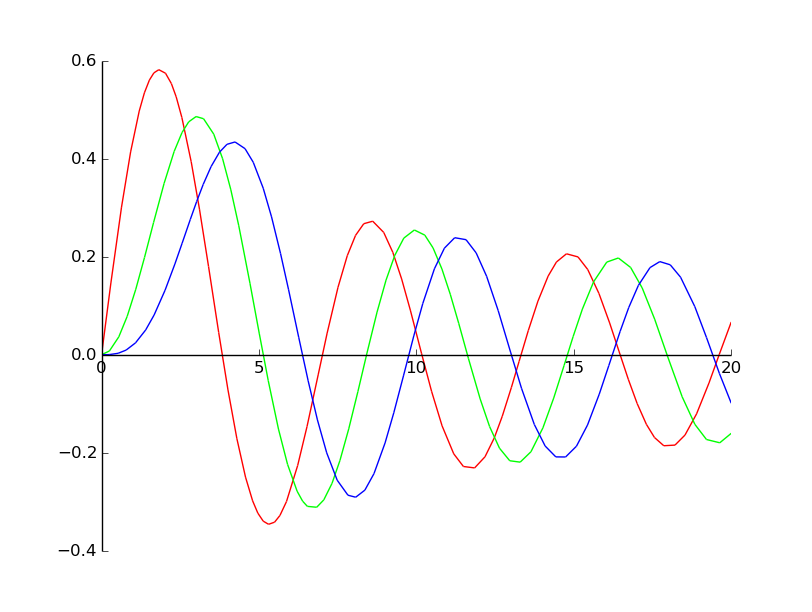
\includegraphics[scale=.5]{imagenes/bessel.png}
\end{center}

\caption{Funciones de Bessel $J_p$, $p=1,2,3$}\label{fig:bessel}

\end{figure}





Ahora consideremos la solución $m=-p$ de la ecuación indicial.
\begin{lstlisting}
>>> Ecuaciones2=[ec.subs(m,Sol_Ecua_Ind[0]) for ec in Ecuaciones]
>>> for i in range(1,orden):
...     iter=solve(Ecuaciones2[i],a[i])[0].factor()
...     print repr(a[i])+'='+repr(iter)
... 
a1=0
a2=a0/(4*(p - 1))
a3=a1/(3*(2*p - 3))
a4=a2/(8*(p - 2))
a5=a3/(5*(2*p - 5))
a6=a4/(12*(p - 3))
a7=a5/(7*(2*p - 7))

\end{lstlisting}
Estas relaciones siguen el mismo patrón que la relación de recurrencia \eqref{eq:recu_bessel} con $-p$ en lugar de $p$. No obstante, la situación para la raíz $-p$ no es exactamente igual a la de la raíz $p$. La diferencia radica en que cuando $p\in\frac12\mathbb{N}=\frac12,1,\frac32,\ldots$  la expresión en el denominador en la relación
\boxedeq{a_{2n}=\frac{a_{2n-2}}{4n(p-n)}}{eq:rel_recu_bess-p}
se puede anular y esto  impediría que pasasemos de miembro esta expresión como hicimos. Notar que este problema ocurre cuando la diferencia de las dos raíces $p-(-p)=2p$ es un entero positivo.  Esto último lo remarcamos porque veremos más adelante que en general es un problema que la diferencia de las raíces de la ecuación indicial sean negativas. También $p=0$ es una situación problemática, dado que en este caso $p=-p$ y por consiguiente no estamos en condiciones de encontrar una solución linealmente independiente de $J_0$. En síntesis $p=0,\frac12,1,\frac32,\ldots$ son valores problemáticos para $p$. 

Cuando $p$ no es uno de los valores problemáticos, estamos en condiciones de definir
\begin{definicion}\label{def:bessel_segunda} Definimos la función de Bessel de primera especie $J_{-p}$ ($p\notin\frac12\mathbb{N}$) como
\[J_{-p}(x)=\sum_{n=0}^{\infty}\frac{(-1)^n}{n!\Gamma(-p+n+1)}\left(\frac{x}{2}\right)^{2n-p}\]
\end{definicion}
Grafiquemos algunas de estas funciones de Bessel.
\begin{sagecommandline}
sage: p1=plot(J(x,-1/3),(x,0,35),ymin=-2,ymax=2,rgbcolor=(1,0,0))
sage: p2=plot(J(x,-2/3),(x,0,35),ymin=-2,ymax=2,rgbcolor=(0,1,0))
sage: p3=plot(J(x,-5/3),(x,0,35),ymin=-2,ymax=2,rgbcolor=(0,0,1))
\end{sagecommandline}
\begin{figure}[h]
\sageplot[scale=.5]{p1+p2+p3}
\caption{Funciones de Bessel $J_{-1/3}$, $J_{-2/3}$ y $J_{-5/3}$.} 
\end{figure}
Más adelante vamos a seguir estudiando con más profundidad la ecuación de Bessel.

\subsection{Teorema fundamental sobre puntos singulares regulares}\label{eq:sec_teor_fund_frob}
Habiendo visto algunos ejemplos, ahora pasaremos a discutir la situación general del método de Frobenius. 

Supongamos $x=0$ un punto regular singular de la ecuación
\begin{equation}\label{eq:dif_2_orden} y''+p(x)y'+q(x)y=0.
\end{equation}
Supongamos que $xp(x)$ y $x^2q(x)$ poseen los  siguientes desarrollos en serie 
\[xp(x)=\sum_{n=0}^{\infty}p_nx^n\quad\text{y}\quad x^2q(x)=\sum_{n=0}^{\infty}q_nx^n\]
Proponemos como solución
\[y=x^{m}\sum_{n=0}^{\infty}a_nx^n=\sum_{n=0}^{\infty}a_nx^{m+n}.\]
Empecemos por hallar las relaciones de recurrencia para los coeficientes $a_n$, $n=0,1,\ldots$.   Tenemos
\begin{subequations}
    \begin{align}
      y'&=\sum_{n=0}^{\infty}(m+n)a_{n}x^{m+n-1}\\
      y''&=\sum_{n=0}^{\infty}(m+n)(m+n-1)a_{n}x^{m+n-2}\notag\\
&=x^{m-2}\sum_{n=0}^{\infty}(m+n)(m+n-1)a_{n}x^{n}\label{eq:der_seg} .
    \end{align}
  \end{subequations}
Luego

\begin{equation}\label{eq:der_pri}
  \begin{split}
    p(x)y'(x)&=\frac{1}{x}\left(\sum_{n=0}^{\infty}p_nx^n\right)\left(\sum_{n=0}^{\infty}(m+n)a_{n}x^{m+n-1}\right)\\
&=x^{m-2}\left(\sum_{n=0}^{\infty}p_nx^n\right)\left(\sum_{n=0}^{\infty}(m+n)a_{n}x^{n}\right)\\
&= x^{m-2}\sum_{n=0}^{\infty}\left(\sum_{k=0}^np_{n-k}(m+k)a_k\right)x^n\\
&= x^{m-2}\sum_{n=0}^{\infty}\left(\sum_{k=0}^{n-1}p_{n-k}(m+k)a_k+p_0(m+n)a_n\right)x^n
  \end{split}
\end{equation}
Ahora desarrollemos $q(x)y(x)$,
\begin{equation}\label{eq:der_cero}
  \begin{split}
    q(x)y(x)&=\frac{1}{x^2}\left(\sum_{n=0}^{\infty}q_nx^n\right)\left(\sum_{n=0}^{\infty}a_{n}x^{m+n}\right)\\
&=x^{m-2}\left(\sum_{n=0}^{\infty}q_nx^n\right)\left(\sum_{n=0}^{\infty}a_{n}x^{n}\right)\\
&= x^{m-2}\sum_{n=0}^{\infty}\left(\sum_{k=0}^nq_{n-k}a_k\right)x^n\\
&= x^{m-2}\sum_{n=0}^{\infty}\left(\sum_{k=0}^{n-1}q_{n-k}a_k+q_0a_n\right)x^n
  \end{split}
\end{equation}
A partir de \eqref{eq:dif_2_orden}, \eqref{eq:der_cero},\eqref{eq:der_pri} y \eqref{eq:der_seg} obtenemos
\begin{equation}
\begin{split}
  0=&x^{m-2}\sum_{n=0}^{\infty}\bigg\{\left[(m+n)(m+n-1)+p_0(m+n)  +q_0  \right] a_{n}\\&+\sum_{k=0}^{n-1}a_k\left[p_{n-k}(m+k) +
q_{n-k}\right]\bigg\}x^n.
\end{split}
\end{equation}
Entonces se debe satisfacer
\boxedeq{\left[(m+n)(m+n-1)+p_0(m+n)  +q_0  \right] a_{n}+\sum_{k=0}^{n-1}a_k\left[p_{n-k}(m+k) +
q_{n-k}\right]=0,}{eq:recu_gral_frob}
para $n=0,1,\ldots$. Definamos
\boxedeq{f(m)=m(m-1)+p_0m+q_0.}{eq:func_f}
Entonces las ecuaciones \eqref{eq:recu_gral_frob} se escriben
\boxedeq{f(m+n)a_n=-\sum_{k=0}^{n-1}a_k\left[p_{n-k}(m+k) +
q_{n-k}\right],\quad n=0,1,\ldots}{eq:recu_gral_frob_2}
La primera de estas ecuaciones es 
\begin{definicion} Definimos la  ecuación indicial por
\begin{equation}\label{eq:eq_indicial} 
  f(m)=m(m-1)+p_0m+q_0=0.
\end{equation}

\end{definicion}

Si $m$ resuelve la ecuación indicial entonces $m$ resuelve la ecuación \eqref{eq:recu_gral_frob_2} para $n=0$ y el valor de $a_0$ se puede elegir arbitrariamente. 

Supongamos que la ecuación indicial tiene las soluciones $m_2\leq m_1$. Podría ocurrir que las soluciones fueran complejos conjugados, pero no trataremos este caso aquí. Ahora discutamosVeamos  cuando es posible resolver las relaciones de recurrencia \eqref{eq:recu_gral_frob_2}. El único problema que podría ocurrir es que  $f(m+n)=0$ para algún valor de $n=1,2,\ldots$, dado que en ese caso \eqref{eq:recu_gral_frob_2} se reduce a 
\begin{equation}\label{eq:ec_enter} 0=-\sum_{k=0}^{n-1}a_k\left[p_{n-k}(m+k) +
q_{n-k}\right].
\end{equation}
Esta ecuación no nos dice nada sobre $a_n$ y no podemos esperar que se satisfaga. Sin embargo, cuando $m=m_1$ esta desafortunada situación no se da, de lo contrario  $m_1+n$ sería una raíz de la ecuación indicial distinta que $m_2$ y $m_1$. En consecuencia, \emph{si $m=m_1$ y $a_0\neq 0$ es elegido arbitrariamente las ecuaciones \eqref{eq:recu_gral_frob_2} determinan los coeficientes $a_n$, $n=1,2,\ldots$.}

Cuando $m=m_2$ si puede ocurrir que $f(m_2+n)=0$, esto es así cuando $m_2+n=m_1$ para algún $n=1,2,\ldots$, vale decir cuando $m_1-m_2\in\mathbb{Z}$.  Luego estamos en condiciones de afirmar que \emph{si $m=m_2$, $m_1-m_2\notin \mathbb{Z}$ y $a_0\neq 0$ es elegido arbitrariamente las ecuaciones \eqref{eq:recu_gral_frob_2} determinan los coeficientes $a_n$, $n=1,2,\ldots$.} En esta situación, se demuestra con facilidad que las dos soluciones obtenidas por el método de Frobenius son linealmente independientes. Por ejemplo, si estas soluciones son
\[y_1=x^{m_1}\sum_{n=0}^{\infty}a_nx^n\quad\text{y}\quad y_2=x^{m_2}\sum_{n=0}^{\infty}n_nx^n,\]
con $a_0\neq 0\neq b_0$ y si suponemos que ellas son linealmente dependientes entonces su cociente $y_1/y_2$ sería una constante $c$  no nula. Pero tomando límite en la expresión $y_1/y_2$ cuando $x\to 0$ vemos que
\[c=\lim_{x\to 0} \frac{y_1}{y_2}=\lim_{x\to 0} x^{m_1-m_2}\frac{\sum_{n=0}^{\infty}a_nx^n}{ \sum_{n=0}^{\infty}b_nx^n  }=0.\frac{a_0}{b_0}=0.\]

Si $m_1-m_2:=n_0\in\mathbb{Z}$, entonces la situación es diferente. Si, en particular,  \emph{tuviesemos $n_0=0$ ( $m_1=m_2$) entonces claramente podremos encontrar esencialemente sólo una solución en serie de Frobenius.}   




Supongamos $n_0>0$.  Cuando $n=n_0$ la ecuación de recurrencia  \eqref{eq:recu_gral_frob_2} se convierte, como ya se dijo, en \eqref{eq:ec_enter} con $m_2$ en lugar de $m$.\label{pag:apar_sol} Una aparente solución sería tomar  $0=a_0=\cdots=a_{n_0-1}$ que resolvería la ecuación conflictiva. Podríamos elegir $a_{n_0}\neq 0$ arbitrariamente y continuar la iteración
\begin{equation}\label{eq:iter_m1}
  \begin{split}
    f(m_1+1)a_{n_0+1}&=-\sum_{k=0}^{n_0}a_k\left[p_{n_0+1-k}(m_2+k) + q_{n_0+1-k}\right]=-a_{n_0}[p_1m_1+q_1]\\
   f(m_1+2) a_{n_0+2}&=-\sum_{k=0}^{n_0+1}a_k\left[p_{n_0+2-k}(m_2+k) + q_{n_0+2-k}\right]\\
                   &=-a_{n_0}[p_2m_1+q_2]-a_{n_0+1}[p_1(m_1+1)+q_0]\\
                   &\,\,\,\vdots
  \end{split}
\end{equation}
Como se ve, la iteración termina siendo la misma que la correpondiente iteración para la raíz $m_1$. Además tendríamos que el desarrollo en serie
\[y(x)=x^{m_2}\sum_{n=0}^{\infty}a_nx^n=x^{m_2}\sum_{n=n_0}^{\infty}a_nx^n
 =x^{m_2+n_0}\sum_{n=0}^{\infty}a_{n+n_0}x^n
=x^{m_1}\sum_{n=0}^{\infty}b_nx^n
,\]
donde $b_n:=a_{n+n_0}$ resuelve el esquema de iteración \eqref{eq:iter_m1} que, como dijimos, es el esquema de iteración correspondiente a $m=m_1$. Vale decir que elegir  $0=a_0=\cdots=a_{n_0-1}$ nos lleva a una solución linealmente dependiente con la solución que ya encontramos para $m=m_1$. Podríamos tener la suerte que eligiendo $a_0\neq 0$ se satisfaga la ecuación \eqref{eq:ec_enter} con $m=m_2$ y $n=n_0$. Si esto ocurre podemos elegir $a_{n_0}$ arbitrariamente, por ejemplo $a_{n_0}=0$, y continuar la iteración. Obtenemos una solución que es linealmente independiente   de la correspondiente a $m_1$. En síntesis, \emph{si $n_0:=m_1-m_2\in\mathbb{Z}$, si $a_0\neq 0$ es eligido arbitrariamente, si  $a_1,\ldots,a_{n_0-1}$ son hallados mediante \eqref{eq:recu_gral_frob} y si se satisface  \eqref{eq:ec_enter} tenemos una segunda solución en serie de Frobenius para $m=m_2$}

Si falla esta última condición ya no hay otra solución en serie de Frobenius. Se puede encontrar un desarrollo, que ya no constituye una serie de Frobenius,  para otra solución de la siguiente forma empleando el método de reducción de orden a partir de la solución conocida $y_1=x^{m_1}\sum_{n=0}^{\infty}a_nx^n$. Este método no decía que la otra solución venía dada a partir de las relaciones
\[y_2(x)=v(x)y_1(x),\quad\text{donde  } v'(x)=\frac{1}{y_1^2}e^{-\int p(x)dx}.\]  
Teniendo en cuenta que
\[p(x)=\sum_{n=0}^{\infty}p_nx^{n-1}=\frac{p_0}{x}+p_1+p_2x+\cdots.\]
Vemos que
\[
   \begin{split}
     v'(x)&=\frac{1}{x^{2m_1}\left(\sum_{n=0}^{\infty}a_nx^n\right)^2}e^{-\int \left(\frac{p_0}{x}+p_1+p_2x+\cdots \right)dx}\\
  &= \frac{1}{x^{2m_1}\left(\sum_{n=0}^{\infty}a_nx^n\right)^2}e^{-p_0 \ln x -p_1x-\cdots }\\
  &= \frac{1}{x^{2m_1+p_0}\left(\sum_{n=0}^{\infty}a_nx^n\right)^2}e^{ -p_1x-\cdots }
   \end{split}
\]

Ahora la función
\[
  g(x)= \frac{ e^{ -p_1x-\cdots } }{\left(\sum_{n=0}^{\infty}a_nx^n\right)^2},
\]
es analítica en $0$ puesto que el denominador no se anula en cero. Por consiguiente tenemos un desarrollo en serie
\[ g(x)=\sum_{n=0}^{\infty}b_nx^n, \quad b_0\neq 0.\]
En la práctica encontrar este desarrollo en serie de manera explícita puede ser muy difícil. Llamemos $k:=2m_1+p_0$. Por la conocida fórmula para la suma de las raíces de una ecuación de segundo grado, se tiene que $m_1+m_2=1-p_0$.  Luego  $2m_1+p_0=2m_1+1-m_1-m_2=m_1-m_2+1\in\mathbb{N}$. 

Tenemos que
\[v'(x)=\frac{b_0}{x^k}+ \frac{b_1}{x^{k-1}}+\cdots+\frac{b_{k-1}}{x}+b_{k}+\cdots\]
Entonces
\[v(x)=\frac{b_0}{(-k+1)x^{k-1}}+ \frac{b_1}{(-k+2)x^{k-2}}+\cdots+b_{k-1}\ln x+b_{k}x+\cdots\]
Reemplazando esta identidad en la expresión para $y_2$,
\[
   \begin{split}
     y_2&=vy_1\\
&=y_1\left(\frac{b_0}{(-k+1)x^{k-1}}+ \frac{b_1}{(-k+2)x^{k-2}}+\cdots+b_{k-1}\ln x+b_{k}x+\cdots\right)\\
       &=b_{k-1}\ln x y_1+ x^{m_1}\sum_{n=0}^{\infty}a_nx^n\left(\frac{b_0}{(-k+1)x^{k-1}}+ \frac{b_1}{(-k+2)x^{k-2}}\cdots\right)\\
       &=b_{k-1}\ln x y_1+ x^{m_1-k+1}\sum_{n=0}^{\infty}a_nx^n\left(\frac{b_0}{(-k+1)}+ \frac{b_1}{(-k+2)}x+\cdots\right)\\
   \end{split}
\]
Ahora $m_1-k+1=m_1-2m_1-p_0+1=-p_0-m_1+1$. Es sabido que la suma de las raices $m_1+m_2$ es igual a $-p_0+1$, es decir $m_1=-p_0+1-m_2$. Entonces $m_1-k+1=m_2$. Obtenemos una solución de la forma
\boxedeq{y_2(x)=b_{k-1}y_1\ln x+x^{m_2}\sum_{n=0}^{\infty}c_nx^n.}{eq:des_enter}
La segunda solución $y_2$ es la suma de una serie de Frobenius, con $m=m_2$, y un multiplo de la función $y_1\ln x$. Esta última función no se puede desarrollar en serie de potencias alrededor de $0$.

Hemos discutido con cierto detalle las posibles soluciones de las ecuaciones de recurrencia. No resta considerar la cuestión de la convergencia de las series. Esto lo tratamos en el siguiente teorema. 

\begin{teorema} Supongamos $x=0$ un punto regular singular de la ecuación
\begin{equation}\label{eq:dif_2_orden} y''+p(x)y'+q(x)y=0.
\end{equation}
Supongamos que $xp(x)$ y $x^2q(x)$ poseen los  siguientes desarrollos en serie 
\[xp(x)=\sum_{n=0}^{\infty}p_nx^n\quad\text{y}\quad x^2q(x)=\sum_{n=0}^{\infty}q_nx^n\]
y que estas series convergen para $|x|<R$ ($R>0$). Supongamos que la ecuación indicial tiene la raíces reales $m_1$, $m_2$ con  $m_2\leq m_1$.  Entonces la ecuación \eqref{eq:dif_2_orden}  tiene una solución en serie de Frobenius dada por
\[y_1=x^{m_1}\sum_{n=0}^{\infty}a_nx^n\quad a_0\neq 0.\]
La serie $\sum_{n=0}^{\infty}a_nx^n$ converge en $|x|<R$. Si $m_1-m_2$ no es un entero no negativo entonces tenemos una segunda solución en serie de Frobenius con $m_2$ en lugar de $m_1$ y satisfaciendo las mismas condiciones que la primer serie.  
\end{teorema}
\begin{demo} Dado que $m_1$ y $m_2$ son raíces de la ecuación indicial vale la factorización
\[f(m)=(m-m_1)(m-m_2)=m^2-(m_1+m_2)m+m_1m_2.\]
Entonces
\[f(m_1+n)=n(n+m_1-m_2)\quad\text{y}\quad f(m_2+n)=n(n+m_2-m_1).\]
Luego
\begin{equation}\label{eq:desig_aux}|f(m_1+n)|\geq n(n-|m_1-m_2|)\quad\text{y}\quad f(m_2+n)\geq n(n-|m_1-m_2|).
\end{equation}
Tomemos $r$ tal que $0<r<R$. Por las mismas razones expresadas  en el Teorema \eqref{eq:teor_ptos_ord},  existe $M>0$ tal que
\[ |p_n|r^n,|q_n|r^n\leq M.\]
Usando \eqref{eq:recu_gral_frob_2}, con $m=m_1$, \eqref{eq:desig_aux} y las desigualdades de arriba concluímos
\[n(n-|m_1-m_2|)|a_n|\leq M\sum_{k=0}^{n-1}\frac{|a_k|}{r^{n-k}}(|m_1|+k+1).\]
Ahora definimos la sucesión $b_n$ por $b_n=|a_n|$, para $0\leq n\leq|m_1-m_2|$ y para $ n>|m_1-m_2|$
\begin{equation}\label{eq:bn_iter}n(n-|m_1-m_2|)b_n= M\sum_{k=0}^{n-1}\frac{b_k}{r^{n-k}}(|m_1|+k+1).\end{equation}
Por una variación simple  del Lema \ref{lema:comp_recu} tenemos que $|a_n|\leq b_n$, para todo $n=0,1,\ldots$. Ahora veremos que la serie $\sum_{n=0}^{\infty}b_nx^n$ converge para  $|x|<r$. Por \eqref{eq:bn_iter} tenemos que
\[ 
   \begin{split}
     r(n+1)(n+1-|m_1-m_2|)b_{n+1}&=M\sum_{k=0}^{n}\frac{|b_k|}{r^{n-k}}(|m_1|+k+1)\\
&=M\sum_{k=0}^{n-1}\frac{b_k}{r^{n-k}}(|m_1|+k+1)+Mb_n(|m_1|+n+1)\\
&=n(n-|m_1-m_2|)b_n+Mb_n(|m_1|+n+1).
  \end{split}
\]

Luego
\[\frac{b_{n+1}}{b_n}=\frac{ n(n-|m_1-m_2|)+M(|m_1|+n+1) }{ r(n+1)(n+1-|m_1-m_2|)  }\]
Y así
\[ \begin{split}
\lim_{n\to\infty}\frac{b_{n+1}|x|^{n+1}}{b_n|x|^n}&=|x|\lim_{n\to\infty}\frac{ n(n-|m_1-m_2|)+M(|m_1|+n+1) }{ r(n+1)(n+1-|m_1-m_2|)  }=\frac{|x|}{r}
\end{split}
\]
Luego la serie  $\sum_{n=0}^{\infty}b_nx^n$   converge para $|x|<r$. Como $|a_n|\leq b_n$ tendremos que  $\sum_{n=0}^{\infty}a_nx^n$ converge absolutamente para $|x|<r$. Finalmente como $0<r<R$ fue elegido arbitrariamente tendremos que la convergencia se da para $|x|<R$. 

Restaría considerar el caso $m=m_2$ cuando $m_1-m_2$ no es entero. Pero la demostración del mismo sigue el mismo camino que para $m=m_1$.

\end{demo}

\subsection{Funciones de Bessel  de segunda especie}

En la subsección \ref{sec:bessel_1} discutimos sobre soluciones de la ecuación de Bessel de orden $p\geq 0$. Obtuvimos la solución en serie de Frobenius asociada a la solución de la ecuación indicial $m=p$ \eqref{eq:sol_ec_ind}, dada en la Definición \ref{def:bessel_primera}. Esta solución es llamada función de Bessel de primera especie y es denotada por $J_p$. Es bueno decir que esta función es continua en $0$ y $J_p(0)=0$. Para la segunda solución de la ecuación indicial $m=-p$, hemos dicho también que para $p\neq 0,\frac12,1,\frac32,\ldots$ hay otra solución linealmente independiente de $J_p$. Esta solución se denomina también función de Bessel de primera especie, se denota $J_{-p}$ y es una función no acotada en $0$.  Según lo que hemos expresado en la Subsección \ref{eq:sec_teor_fund_frob}, aún en el caso $p=0,\frac12,1,\frac32,\ldots$ tenemos esperanzas de encontrar una solución en serie de Frobenius o al menos una solución de la forma \eqref{eq:des_enter}. Este tipo de soluciones es lo que discutiremos en esta subsección. 

Empecemos suponiendo $p$ entero positivo. A partir de \eqref{eq:recu_-p} sabemos que la fórmula de recurrencia para $m=-p$ es
\boxedeq{n(2p-n) a_{n} = a_{n-2},\quad n\geq 2}{eq:rel_recu_-p}
También recordemos de \eqref{eq:rel_recu_-p_a}  la ecuación
\[-a_1(2p-1)=0,\]
que  implica $a_1=0$, puesto que $p$ es entero y por ende $p\neq\frac12$. Como consecuencia de la relación de recurrencia  \eqref{eq:rel_recu_-p} tenemos $a_n=0$ para todo $n$ impar. Para afirmar esto último tomamos en cuenta que al ser $p$ entero  $2p-n\neq 0$ cuando $n$ es impar.   Cuando  $n$ es par y más en concreto $n=2p$ la relación de recurrencia \eqref{eq:rel_recu_-p} toma la forma $a_{n-2}=0$. Ahora si $a_{n-2}=0$ entonces \eqref{eq:rel_recu_-p} implica que $a_{n-4}=a_{n-6}=\cdots a_0=0$. Eligiendo $a_n$ arbitrariamente y al resto de los $a_k$ con $k$ par mayor a $n$ de modo que se satisfaga la relación de recurrencia se llega a una solución en serie de Frobenius. Lamentablemente esta segunda solución es esencialmente la misma  que $J_p$. Esto ya lo hemos discutido en sección \vref{pag:apar_sol}.  De modo que cuando $p$ es entero positivo no tenemos una segunda solución en serie de Frobenius. 

Más adelante volveremos al caso $p$ entero. Ahora consideremos $p=\frac{2k+1}{2}$ con $k$ entero $k\geq 0$.  Reemplazando $p$ en \eqref{eq:rel_recu_-p}  por este valor y reemplazando $n$ por $2k+1$, concluímos $a_{2k-1}=0$. Ahora iterando la relación de recurrencia $a_{2k-3}=\cdots=a_1=0$. La situación es parecida al caso anterior, podemos elegir $a_{2k+1}$ libremente, vamos a elegirlo igual a $0$. Esto anula todos los coeficientes $a_n$ con $n$ impar. Pero la diferencia con el caso anterior es que podemos elegir libremente $a_0$. Llegamos así a la misma solución de la Definición \ref{def:bessel_segunda}. En síntesis \emph{para todo $p$ que no es un entero no negativo, tenemos el par de soluciones linealmente independientes $J_p$ y $J_{-p}$ tales que
\boxedeq{y=c_1J_p+c_2J_{-p}}{eq:sol_gen_bessel_1}
es la solución general de la ecuación de Bessel}

Ahora volvamos al caso $p\in\mathbb{Z}$ para encontrar una segunda solución  linealmente independiente de $J_p$. Podríamos buscar esta solución apelando a la expresión \eqref{eq:des_enter}, pero es costumbre buscar de otra manera esta segunda solución y vamos a discutir brevemente,  sin justificar todos los detalles,  esta otra forma. La idea es expresar la segunda solución para  $p=n\in\mathbb{Z}$ como límite de soluciones  de la forma  \eqref{eq:sol_gen_bessel_1} cuando $p\to n$. Más concretamente.

\begin{definicion} Para $p\notin\mathbb{Z}$ definimos la función de Bessel $Y_p$ de segunda especie por
\begin{equation}\label{eq:bessel_2_especie}
Y_p=\frac{\cos p\pi J_p-J_{-p}}{\sen p\pi}.
\end{equation}
\end{definicion}

La función $Y_p$ es una solución puesto que es una expresión del tipo \eqref{eq:sol_gen_bessel_1}. Además es no acotada cerca de $0$ dado que $J_p$ es acotada y $J_{-p}$ no. La razón de esta llamativa definición es el siguiente resultado. 

\begin{lema} Para $n$ entero no negativo,  el  límite $\lim_{p\to n}Y_p$ existe. Por consiguiente, podemos definir
\begin{equation}\label{eq:bessel_2_especie_b}
Y_n(x):=\lim_{p\to n}Y_p(x).
\end{equation}  
Esta función es solución de la ecuación de Bessel de orden $n$ y se denomina, también, función de Bessel de segunda especie. También resulta ser una función no acotada cerca de $0$ y por consiguiente, linealmente idependiente de $J_n$.
\end{lema}





\end{document}


\printindex

\end{document}
